\documentclass[
paper = a4,
fontsize = 12pt,
headinclude = true,
% start chapters on the right side
open = right,
% Use twosided layout? Every chapter starts on the right side, therefore sometimes blank pages are added between chapters.
twoside = false,
BCOR = 10mm,
% add lists and bibliography to table of contents
toc = listofnumbered,
toc = bibnumbered,
% enumerate chapters as x.y instead of x.y.
numbers = noendperiod
]{scrreprt}
\renewcommand{\familydefault}{\sfdefault}

%-------------------------------------------------------------------------------------------%
% PACKAGES 
\usepackage[ngerman]{babel}
\usepackage[german=quotes]{csquotes}
\usepackage{tabularx}
\usepackage[hidelinks]{hyperref}
\usepackage{amsmath} % for math
\usepackage{amssymb}
\usepackage{graphicx} % for images
\usepackage{subcaption} % for images
\usepackage{float}
\usepackage[utf8]{inputenc} 
\usepackage{booktabs}
\usepackage{longtable} % multipage tables
\usepackage[automark]{scrlayer-scrpage}
\usepackage{parskip} % turn off indents
\usepackage{listings} % code segments
\usepackage[table,xcdraw]{xcolor} % colors for listing format config
%%Java Code im Stil von Eclipse
\definecolor{javared}{rgb}{0.6,0,0} % for strings
\definecolor{javagreen}{rgb}{0.25,0.5,0.35} % comments
\definecolor{javapurple}{rgb}{0.5,0,0.35} % keywords
\definecolor{javadocblue}{rgb}{0.25,0.35,0.75} % javadoc
  
\lstdefinestyle{Java}{language=Java,
	basicstyle=\footnotesize\ttfamily,
	keywordstyle=\color{javapurple}\bfseries,
	stringstyle=\color{javared},
	commentstyle=\color{javagreen},
	morecomment=[s][\color{javadocblue}]{/**}{*/},
	numbers=left,
	numberstyle=\small\color{black},
	stepnumber=1,
	numbersep=10pt,
	tabsize=4,
	showspaces=false,
	showstringspaces=false,
	breaklines=true,
	frame=single
}


% HTML Code Style
\definecolor{htmlblue}{HTML}{2a71b8} % for tags
\definecolor{htmlpurple}{HTML}{703fa6} % for "" enclosed
\definecolor{htmlpink}{HTML}{e97bdb} % unused

\lstdefinelanguage{HTML}{
	sensitive=true,
	keywords={html, title, meta, style, head, body, h1, h2, h3, p},
	otherkeywords={<, >, /},
	morestring=[b]"
}

\lstdefinestyle{HTML}{language=HTML,
	basicstyle=\footnotesize\ttfamily,
	keywordstyle=\color{htmlblue}\bfseries,
	stringstyle=\color{htmlpurple},
	numbers=left,
	numberstyle=\small\color{black},
	stepnumber=1,
	numbersep=10pt,
	tabsize=4,
	showspaces=false,
	showstringspaces=false,
	breaklines=true,
	frame=single
}
	
	

%%Python Code im Stil von Eclipse
\definecolor{red}{rgb}{1,0,0} % keywords

\lstdefinestyle{Python}{language=Python,
	basicstyle=\ttfamily,
	keywordstyle=\color{javapurple}\bfseries,
	stringstyle=\color{javared},
	commentstyle=\color{javagreen},
	morecomment=[s][\color{javadocblue}]{/**}{*/},
	numbers=left,
	numberstyle=\tiny\color{black},
	stepnumber=1,
	numbersep=10pt,
	tabsize=4,
	showspaces=false,
	showstringspaces=false
}
 % code listing config
\lstset{
	  basicstyle=\footnotesize\ttfamily
}
\renewcommand{\lstlistingname}{Quellcode} % change 'Listing' to 'Quellcode'
\renewcommand{\lstlistlistingname}{Quellcodeverzeichnis}

%\usepackage{pdfpages} % include excel pdf

\usepackage{tocloft}
\setlength\cftbeforechapskip{5pt}
\setlength\cftbeforepartskip{15pt}

\usepackage[export]{adjustbox}

\usepackage{multirow}

\usepackage{marvosym}

\usepackage{circuitikz}
%-------------------------------------------------------------------------------------------%
% BIBLIOGRAPHY
\usepackage[backend=bibtex,style=verbose-trad2]{biblatex}
\bibliography{bibliography/citations_gwercher}
\bibliography{bibliography/citations_egger}

%-------------------------------------------------------------------------------------------%
% VARIABLES
\newcommand{\mytitle}{NWES-SESD} 
\newcommand{\mysubtitle}{-}
\newcommand{\myschool}{Höhere Technische Bundeslehr- und Versuchsanstalt Anichstraße} 
\newcommand{\myinstitute}{Abteilung für Wirtschaftsingenieure/Betriebsinformatik} 
\newcommand{\mysubmissionyear}{2024}
\newcommand{\mysubmissionmonth}{-}
\newcommand{\myauthor}{Gwercher}
\newcommand{\mysupervisor}{-}

\newcommand{\mysubject}{SUBJECT}  %% also used for PDF metadata (hyperref)
\newcommand{\mykeywords}{KEYWORDS}  %% also used for PDF metadata (hyperref)

%-------------------------------------------------------------------------------------------%
% HEADERS & FOOTERS
\newcommand{\normalHeaderFooter}{%
	\ihead*{
\includegraphics[width=0.45\linewidth]{figures/anich_logo.png}}
	\chead*{}
	\ohead*{
\includegraphics[width=0.2\linewidth]{figures/htl_logo.png}}
	
	\ifoot*{\myauthor}
	\cfoot*{}
	\ofoot*{\thepage}
}

\newcommand{\normalFooter}{%
	\ifoot{\myauthor}
	\cfoot{}
	\ofoot{\thepage}
}

\newcommand{\noHeader}{%
	\ihead{}
	\chead{}
	\ohead{}
}

\newcommand{\noFooter}{%
	\ifoot{}
	\cfoot{}
	\ofoot{}
}


\clearpairofpagestyles
\normalHeaderFooter	
\pagestyle{scrheadings}

%-------------------------------------------------------------------------------------------%


\begin{document}
%-------------------------------------------------------------------------------------------%
% PREAMBLE PART
	\noFooter
	\pagenumbering{gobble}
		\begin{center}
	\vspace*{1cm}
	{\huge Matura}\\
	\bigskip
	{\LARGE \mytitle} \\
	\smallskip
	{\large \myschool} \\
	\bigskip
	\hrule
	\bigskip
	{\large \myinstitute} \\
	
	\bigskip
	Ausgeführt im Schuljahr 2024 von: \\
	\myauthor \\
	\bigskip


\end{center}
	
	\normalFooter 
	\pagenumbering{roman} \setcounter{page}{1}
	\tableofcontents
	\newpage
%-------------------------------------------------------------------------------------------%
% MAIN PART
	\pagenumbering{arabic} 
	\setcounter{page}{1}
	
	\part{2BHWII}
	\chapter{Digitaltechnik}
\textbf{Digital:} kann nur bestimmte (diskrete) Werte annehmen (z.B. 0/1, TRUE/FALSE; Digitaluhr 08:35 $\rightarrow$ 08:26 $\rightarrow$ 08:37)

\textbf{Analog:} kann beliebige (kontinuierliche) Werte annehmen (Temperaturmesswerte: 38.089°C, 40.05°C).

Aufgabe: Schaltung, mit zwei Schaltern, mit denen man Licht aus- und einschalten kann
\begin{center}	
\begin{tabular}{cc}
	\begin{circuitikz}[scale=1]
		\draw
		(1,0) node[spdt] (Sw1) {}		
		(2,0) node[spdt, xscale=-1] (Sw2) {}
		
		(Sw1.out 1) to (Sw2.out 1)
		(Sw1.out 2) to (Sw2.out 2)
		
		(0,0) to (Sw1.in)
		(Sw2.in) to (3,0)
		to (3,-1)
		to[lamp] (0,-1)
		
		(0,0) to[battery1] (0,-1)
		;
	\end{circuitikz}
	&
	\begin{tabular}{c|c||c}
		S1 & S2 & L \\
		\hline
		0 & 0 & 1 \\
		0 & 1 & 0 \\
		1 & 0 & 0 \\
		1 & 1 & 0 \\
	\end{tabular}
\end{tabular}
\end{center}	

\textbf{Allgemein}
\begin{itemize}
	\item mehrere Eingänge (a, b, c, d,...) (Schalter)
	\item einen Ausgang (x) (Lampe)
\end{itemize}

\section{Boolsche Algebra}
\textbf{Grundrechenwege} \\
\begin{tabular}{ccc}
	$\bullet$ UND (konjunktion) & \begin{tabular}{c|c||c}
		a & b & a $\land$ b \\
		\hline
		0 & 0 & 0 \\
		0 & 1 & 0 \\
		1 & 0 & 0 \\
		1 & 1 & 1 \\
	\end{tabular} & circuit \\

	& & \\
	
	$\bullet$ ODER (disjunktion) & \begin{tabular}{c|c||c}
		a & b & a $\lor$ b \\
		\hline
		0 & 0 & 0 \\
		0 & 1 & 1 \\
		1 & 0 & 1 \\
		1 & 1 & 0 \\
	\end{tabular} & circuit \\

	& & \\

	$\bullet$ NICHT (disjunktion) & \begin{tabular}{c||c}
		a & $\lnot$a oder $\overline{\text{a}}$ \\
		\hline
		0 & 1  \\
		0 & 0  \\
	\end{tabular} & \\
\end{tabular}


$\text{x}_1$ = a $\land$ (b $\lor$ c) \\
$\text{z}^{\text{Anzahl der Variablen}}$ = $\text{2}^\text{3}$ = 8

\begin{tabular}{c|c|c||c||c}
	a & b & c & b $\lor$ c & $\text{x}_1$ \\
	\hline
	0 & 0 & 0 & 0 & 0\\
	1 & 0 & 0 & 0 & 0\\
	0 & 1 & 1 & 1 & 0\\
	1 & 1 & 1 & 1 & 1\\
	0 & 0 & 1 & 1 & 0\\
	1 & 0 & 1 & 1 & 1\\
	0 & 1 & 1 & 1 & 0\\
	1 & 1 & 1 & 1 & 1\\
\end{tabular}

$\text{x}_2$ = a $\land$ b $\land$ c $\land$ $\overline{\text{a}}$ \\

\begin{tabular}{c|c|c|c||c||c||c}
	a & b & c & $\land$a & a $\land$ b & a $\land$ b $\land$ c & $\text{x}_2$ \\
	\hline
	0 & 0 & 0 & 1 & 0 & 0 & 0 \\
	1 & 0 & 0 & 0 & 0 & 0 & 0 \\
	0 & 1 & 0 & 1 & 0 & 0 & 0 \\
	1 & 1 & 0 & 0 & 1 & 0 & 0 \\
	0 & 0 & 1 & 1 & 0 & 0 & 0 \\
	1 & 0 & 1 & 0 & 0 & 0 & 0 \\
	0 & 1 & 1 & 1 & 0 & 0 & 0 \\
	1 & 1 & 1 & 0 & 1 & 1 & 0 \\
\end{tabular}

$\text{x}_3$ = a $\land$ b $\land$ ($\overline{\text{a}}$ $\lor$ c) \\

\begin{tabular}{c|c|c|c||c||c||c}
	a & b & c & $\overline{\text{a}}$ & (a $\lor$ c) & a $\land$ b & $\text{x}_3$ \\
	\hline
	0 & 0 & 0 & 1 & 1 & 0 & 0 \\
	1 & 0 & 0 & 0 & 0 & 0 & 0 \\
	0 & 1 & 0 & 1 & 1 & 0 & 0 \\
	1 & 1 & 0 & 0 & 0 & 1 & 0 \\
	0 & 0 & 1 & 1 & 1 & 0 & 0 \\
	1 & 0 & 1 & 0 & 1 & 0 & 0 \\
	0 & 1 & 1 & 1 & 1 & 0 & 0 \\
	1 & 1 & 1 & 0 & 1 & 1 & 1 \\
\end{tabular} \\
$\text{x}_3$ = a $\land$ b $\land$ c 

\textbf{Rechenregeln} \\
\begin{itemize}
	\item Vorrangsregeln\\
	$\lnot$ \textgreater $\land$ \textgreater $\lor$
	\item Kommutativgesetz \\
	a $\land$ b = b $\land$ a \\
	a $\lor$ b = b $\lor$ a 
	\item Assoziativgesetz \\
	a $\land$ (b $\land$ c) =(a $\land$ b) $\land$ c \\
	a $\lor$ (b $\lor$ c) =(a $\lor$ b) $\lor$ c
	\item Distributivgesetz \\
	a $\land$ (b $\lor$ c) = (a $\land$ b) $\lor$ (a $\land$ c) \\
	a $\lor$ (b $\land$ c) = (a $\lor$ b) $\land$ (a $\lor$ c)
	\item De Morgan'sche Gesetz \\
	$\overline{\text{a}\land\text{b}}$ = $\overline{\text{a}} \lor \overline{\text{b}}$ \\
	$\overline{\text{a}\lor\text{b}}$ = $\overline{\text{a}} \land \overline{\text{b}}$ 
\end{itemize}




	
	\part{3BHWII}
	\chapter{Bussysteme}
Bei einem Bussystem teilen sich mehrere Teilnehmer (z.B. Arduinos) einen Übertragungsweg.

\subsection*{Grundlegende Eigenschaften}
\begin{itemize}
	\item Übertragungsart
	\begin{itemize}
		\item Seriell: Zeichen werden nacheinander übertragen
		\item Parallel: Zeichen werden gleichzeitig übertragen
	\end{itemize}
	\item Topologie
	\begin{itemize}
		\item Punkt-zu-Punkt
		\item Linientopologie
		\item Sterntopologie
		\item Ringtopologie
		\item Baumtopologie
		\begin{figure}[H]
			\centering
			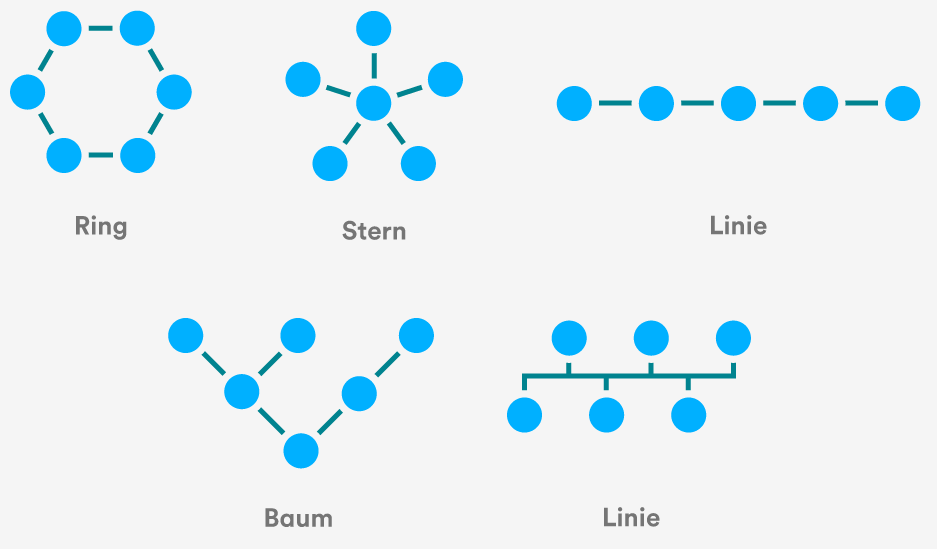
\includegraphics[width=0.7\linewidth]{figures/topo.png}
			\caption{Bustopologiearten}
		\end{figure}
	\end{itemize}
	\item Priorisierung, Kollisionsvermeidung
	\item Synchronisierung
	\begin{itemize}
		\item synchron: eigene Taktleitung
		\item asynchron: keine Taktleitung, fix vorgegebene Übertragungsrate \\
		Einheit: 1 baud = 1 $\dfrac{\text{bit}}{\text{s}}$
	\end{itemize}
	\item Fehlererkennung
\end{itemize}

\textbf{Konkrete Beispiele:} RS-232, CAN, I2C, SPI, USB, Bluetooth

\section{RS-232 (UART)}
RS-232 kann zwei Geräte miteinander verbinden.
\begin{itemize}
	\item Topologie: Punkt-zu-Punkt
	\item Priorisierung, Kollisionsvermeidung: nicht nötig (2 Kabel: 1x Rx, 1x Tx)
	\item Synchronisierung: asynchron
	\item \begin{tabbing}
		Übertragungsart: Seriell ~~~ \= 3 bis 15V '1' \\
		~~~~~~~~~~~~~~~~~~~~~~~~~~~~~~~~ \= -3 bis -15V '0'
	\end{tabbing}
	Achtung: Alle Arduinos nutzen den gleichen GND-Pin!
	\item Fehlererkennung: eventuell mit einem Parity-Bit
\end{itemize}

\subsection*{Konkrete Umsetzung}
Beim RS-232 bestehen die Daten aus einem Startbit, 5-8 Datenbits, dann eventuell ein Parity-Bit und am Ende 1 bis 2 Stopbits

Bsp: 9600 8E1 \\
\begin{tabular}{c|c|c|c}
	9600&8&E&1 \\
	\hline
	Übertragungswert&Anzahl der Datenbits&ein Even-Parity-Bit&Anzahl der Stoppbits \\
\end{tabular}


'a' ASCII, 97 $\rightarrow$ 01100001 \\

\begin{tabular}{c|c|c|c}
	0 & 01100001 & 1 & 1 \\
	\hline
	Start & Datenbits & Parity-bit & Stopp-Bit \\
\end{tabular}

Das Parity-Bit kann
\begin{itemize}
	\item O ... Odd
	\item E ... Even
	\item N ... None
\end{itemize}
sein

Bsp 2: 96000 8O1 \\
'S', 83 $\rightarrow$ 1010011 \quad 0 1010011 1 1 \\
'E', 69 $\rightarrow$ 01000101 \quad 0 1000101 0 1

\subsection*{UART am Arduino}
Der Arduino besitzt ein UART-Bauteil, welches für die aktuelle Kommunikation genutzt werden kann. UART-Bauteil sendet immer mit 8 Datenbits und immer mit einem Stoppbit.

\textbf{Serial Funktionen} \\
\texttt{Serial.available()} ... wandelt eingegebene Zeichen in ASCII-Zeichen/Zahlen um \\
Beispiel mit Ausgabe: HELLO $\rightarrow$ 72 69 76 76 79 10

\texttt{Serial.print()} ... gibt Daten im Serial Monitor aus
\begin{tabbing}
	z.B. \= \texttt{Serial.print(78)} $\rightarrow$ 78 \\
	~~~~~ \= \texttt{Serial.print("Test")} $\rightarrow$ Test 
\end{tabbing}
Weiters kann man Zahlen in anderen Zahlensystemen umwandeln und ausgeben (BIN, OCT, DEC, HEX) 
\begin{tabbing}
	z.B. \= \texttt{Serial.print(78, BIN)} $\rightarrow$ 1001110 \\
	~~~~~ \= \texttt{Serial.print(78, HEX)} $\rightarrow$ 4E 
\end{tabbing}
oder auch auf Nachkommastellen runden:
\begin{tabbing}
	z.B. \= \texttt{Serial.print(1.23456, 0)} $\rightarrow$ 1 \\
	~~~~~ \= \texttt{Serial.print(1.23456, 2)} $\rightarrow$ 1.23 \\
	~~~~~ \= \texttt{Serial.print(1.23456, 4)} $\rightarrow$ 1.2345
\end{tabbing}

\texttt{Serial.println()} ... gleich wie \texttt{Serial.print()}, jedoch beginnt es mit ASCII 13 oder '\textbackslash r' (neue Zeile beginnen) und endet mit ASCII 10 oder '\textbackslash n' (Zeile beenden).

\texttt{Serial.read()} ... gleich wie Serial.available()

\texttt{Serial.write()} ... ähnlich wie \texttt{Serial.print()} und \texttt{Serial.available()} jedoch wird hier ASCII-Zahlen in Buchstaben umgewandelt.
\begin{tabbing}
	z.B. \= \texttt{Serial.write(72)} $\rightarrow$ H \\
	~~~~~ \= \texttt{Serial.write(69)} $\rightarrow$ E \\
	~~~~~ \= \texttt{Serial.write(76)} $\rightarrow$ L \\
	~~~~~ \= \texttt{Serial.write(76)} $\rightarrow$ L \\
	~~~~~ \= \texttt{Serial.write(79)} $\rightarrow$ O \\
	~~~~~ \= \texttt{Serial.write(32)} $\rightarrow$ SPACE
\end{tabbing}

\section{CAN-Bus (Controll Area Network)}
Der CAN-Bus ist ein serieller Bus der speziell für die Automobilindustrie entwickelt wurde.

\subsection*{Aktuelle Anwendungen}
\begin{itemize}
	\item Autos (Vernetzung von Steuergeräten und Sensoren)
	\item Flugzeuge
	\item Raumfahrt
	\item Medizintechnik
	\item ...
\end{itemize}
Der CAN-Bus arbeitet nach dem Multi-Master-Prinzip und bildet eine Linientopologie.

\subsection*{Aufbau}
\begin{figure}[H]
	\centering
	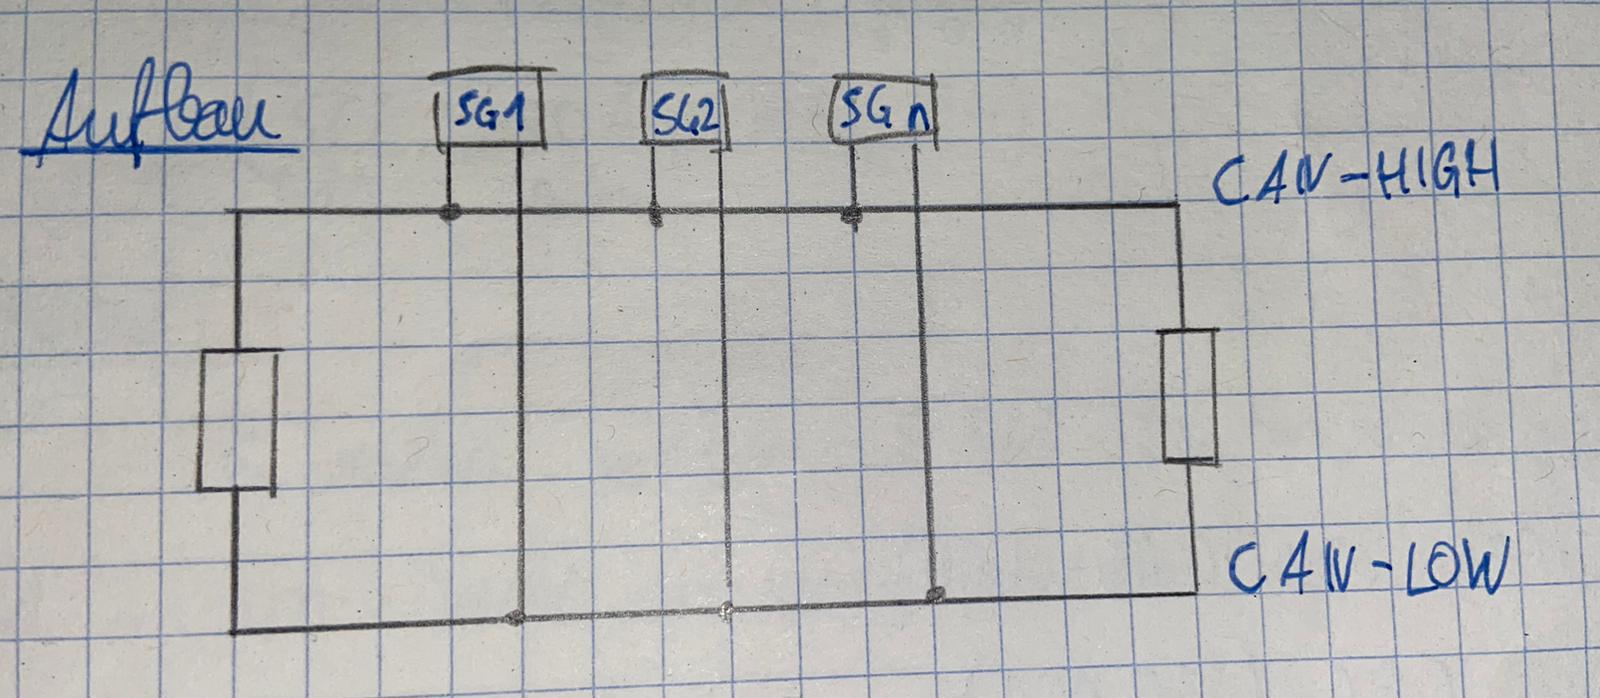
\includegraphics[width=0.8\linewidth]{figures/canbus.jpeg}
	\caption{CAN-Bus Aufbau}
\end{figure}
Der CAN-Bus ist ein asynchroner Bus \\

\begin{tabular}{ccccccc}
	Datenwert & Startbit & 1 & \checkmark && Startbit & 1 \\
	& Message ID & 11 & $\leftarrow$ && Daten & 8 \\
	& Steuerbits & 7 & \checkmark && (Parity & 1) \\
	& Datenbits & 0-64 & \checkmark && Stopp & 1 \\
	& Fehlererkennung & 15 & $\leftarrow$ &&  &  \\
	& Steuerbits & 3 & \checkmark &&  &  \\
	& Stoppbits & 7 & \checkmark &&  &  \\
\end{tabular}

\subsection*{Message ID}
Dort steht um welche Art von Nachricht es sich handelt und wie wichtig die Nachricht ist (z.B. Wasser, Öl, Airbag). Desto kleiner die Message ID ist, desto wichtiger ist die Nachricht. Jedes Sg kann nur eine Message ID aussenden (Priorisierung).

\subsection*{Kollisionsvermeidung CSMA/CR}
SG1: M-ID = 000100 \\
SG2: M-ID = 011011 \\
SG3: M-ID = 001101 \\
0 ... dominant \\
1 ... rezessiv

\subsection*{Sicherheit}
\begin{itemize}
	\item zwei Leitungen (CAN-LOW, CAN-HIGH)
	\item Fehlererkennung mit CRC (15 Bit)
	\item Stuffbit (Stopfbit) Bei fünf gleichen Bits wird ein anderes eingefügt \\
	0000000 \\
	00000100
\end{itemize}

\subsection*{Zusammenfassung}
\begin{itemize}
	\item seriell
	\item Message ID mit CSMA/CR
	\item Linientopologie
	\item asynchron
	\item Stuffbit, CRC, 2 Leitungen
\end{itemize}

\section{I2C-Bus (IIC, I²C)}
Der I2C-Bus wurde Anfang 80er Jahre von der Firma Philips entwickelt. \\
Der I2C-Bus ...
\begin{itemize}
	\item ... ist seriell
	\item ... hat 2 Leiter: SCL \& SDA (Serial Clock, Serial Data)
	\item ... ist synchron
	\item ... funktioniert nach Master-Slave-Prinzip. \\
	Es gibt einen Master (es wären mehrere möglich) $\rightarrow$ keine Kollisionen, Priorisierung unnötig durch Master
\end{itemize}

\subsection*{Aufbau}
\begin{itemize}
	\item Linientopologie
	\item 2 Leitungen mit Pullup-Wiederstände $\rightarrow$ Ruhe zustand HIGH (SCL Takt, SDA Daten; A5, A4)
\end{itemize}

\subsection*{Ablauf}
\begin{itemize}
	\item es werden immer 8 Bit Datenwerte gesendet
	\item um Daten zu senden muss der Pegel der Datenleitung stabil sein (0 oder 1), falls die Taktleitung auf HIGH ist. Sobald die Taktleitung auf LOW ist, kann die Datenleitung das Bit setzen.
	\begin{figure}[H]
		\centering
		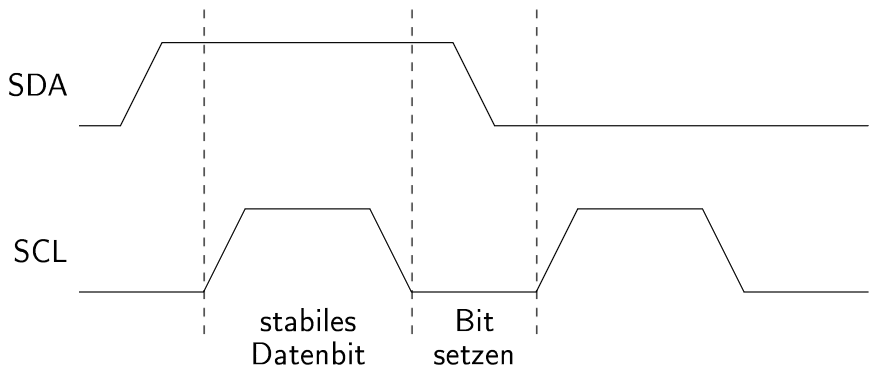
\includegraphics[width=0.8\linewidth]{figures/i2c2.png}
		\caption{I2C-Bus Bitsetzung}
	\end{figure}
	\item Steuersignale
	\begin{itemize}
		\item Startsignal (fallende Flanke, während der Takt auf HIGH ist)
		\item Stopsignal (steigende Flanke, während der Takt auf HIGH ist)
		\begin{figure}[H]
			\centering
			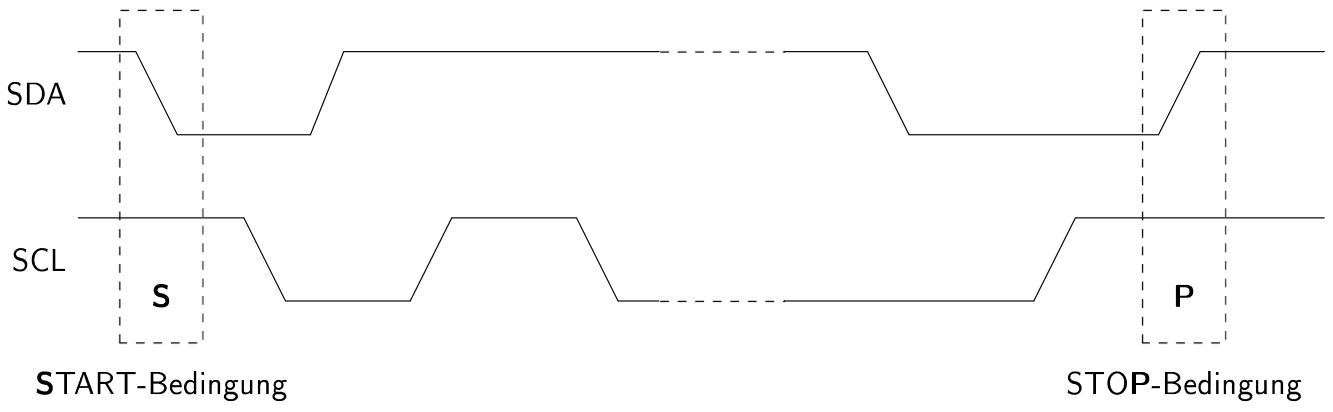
\includegraphics[width=0.8\linewidth]{figures/i2c3.png}
			\caption{I2C-Bus Steuersignale}
		\end{figure}
	\end{itemize}
\end{itemize}

\subsection*{Adressierung}
\begin{itemize}
	\item 7 Bit-Adressen für die Slaves \\
	$\rightarrow$ 128 mögliche Teilnehmer (eig. 112)
	\item 0000000 $\rightarrow$ general call address (Broadcastaddresse)
	\item Das 8te Bit sagt ob der Master lesen oder schreiben soll
\end{itemize}

\begin{figure}[H]
	\centering
	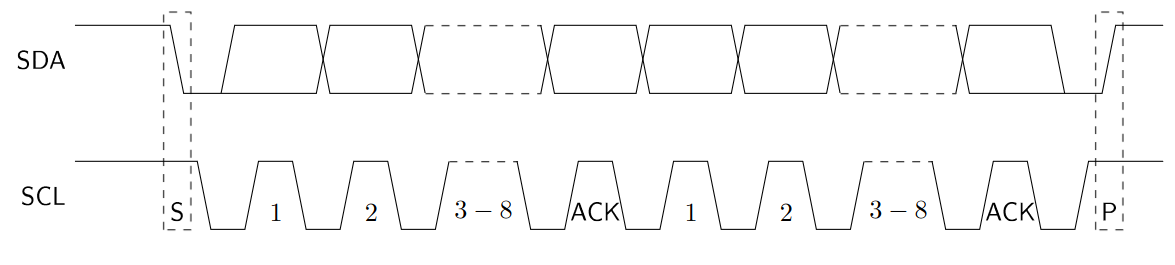
\includegraphics[width=0.8\linewidth]{figures/i2cablauf.png}
	\caption{I2C Ablauf}
\end{figure}

\subsection*{Zusammenfassung}
\begin{itemize}
	\item seriell
	\item Linientopologie
	\item Master-Slave $\rightarrow$ unnötig (bei einem Master)
	\item synchron
	\item ACK, Takt
\end{itemize}

\begin{tabular}{ | p{\dimexpr 0.5\linewidth-2\tabcolsep} | p{\dimexpr 0.5\linewidth-2\tabcolsep} |} \hline
	\textbf{Master} & \textbf{Slave} \\ \hline
	\texttt{Wire.beginTransmission(address);} & \texttt{Wire.begin(address);} \\
	\texttt{Wire.endTransmission();} & \texttt{Wire.onRecieve();} \\
	\texttt{Wire.read();} & \texttt{Wire.onRequest();} \\
	\texttt{Wire.write();} &  \\
	\texttt{Wire.available();} &  \\
	\hline
\end{tabular} 

\iffalse
	\subsection*{I2C-Display (OLED)}
	Bibliotheken installieren: GFX, SSD 1306 (Adafruit), BusIO \\
	Wire $\rightarrow$ I2C Scanner (Adresse auslesen) \\
	SSD 1306 $\rightarrow$ 128x64 I2C 

	\subsection*{OOP am Arduino (C++)}
	Objekt besteht aus
	\begin{itemize}
		\item Attribute, Felder, Eigenschaften
		\item Konstruktor
		\item Funktionen/Methoden
	\end{itemize}
\fi
	\chapter{Finite State Machine (Endlicher Automat)}
Die Finite State Machine ist ein Modell eines Verhaltens. Es ist ein graphischer Entwurf, der flexibel Erweiterbar ist, sowie ein Programmierkonzept.

\textbf{Beispiel Ampel} \\
\begin{enumerate}
	\item Entwurf eines Zustanddiagrammes mit Übergang
	\item Zustand durchnummerieren (wird global gespeichert)
	\item Übergänge sind \texttt{if}-Bedingungen (Ausnahme: sofortige Aktionen)
	\item Zustände sind Methoden: Zeitsensible Übergänge benötigen 2 Zustände (starten und warten)
\end{enumerate}
Ampel: 3s rot, 5s grün
\begin{figure}[H]
	\centering
	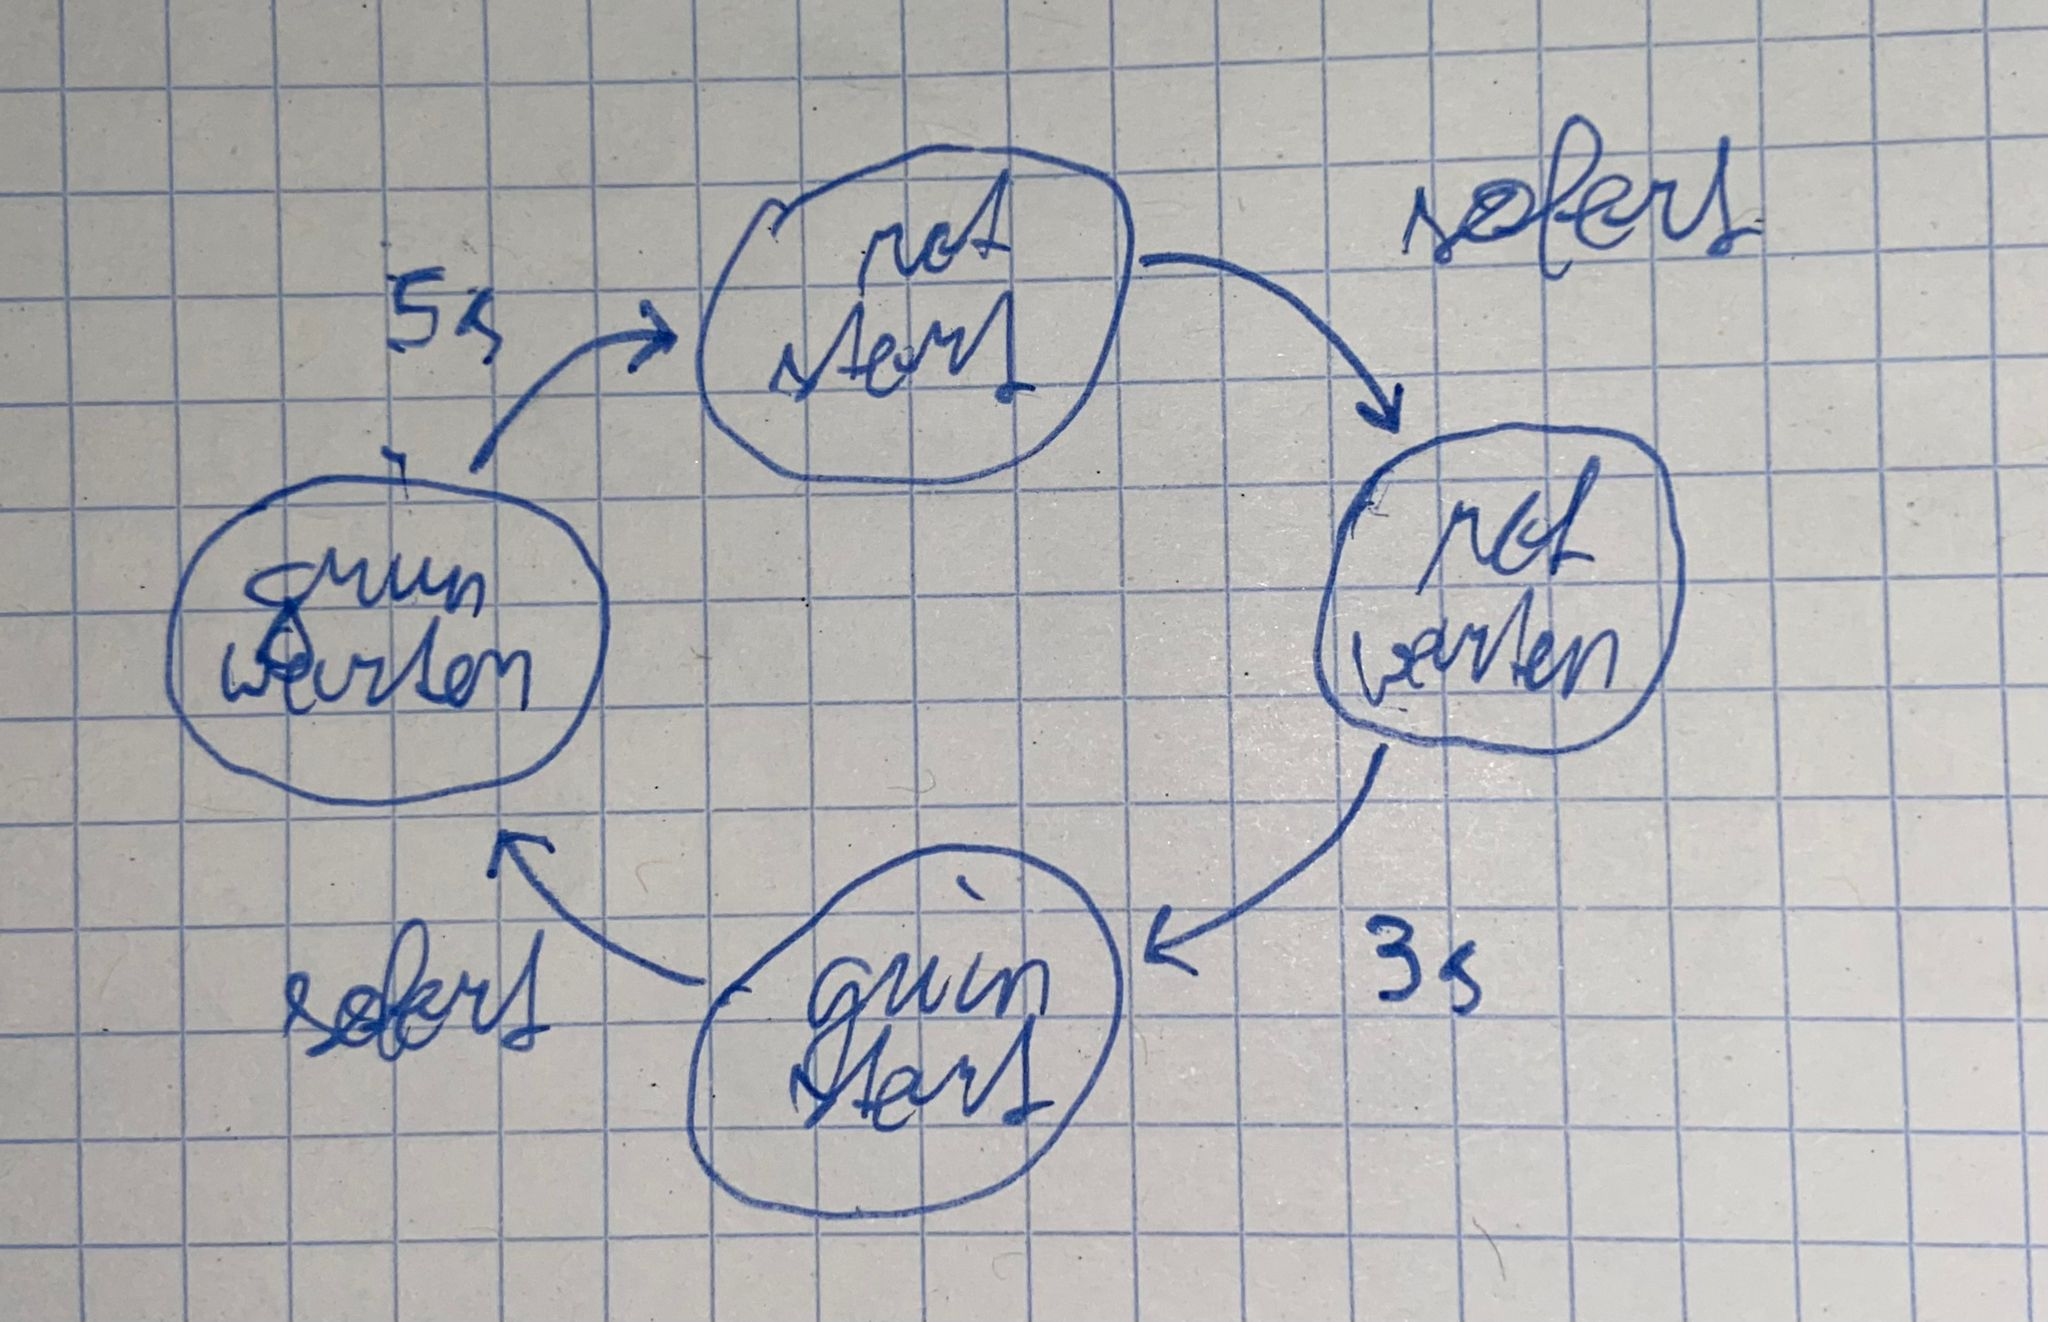
\includegraphics[width=0.8\linewidth]{figures/ampel.jpeg}
	\caption{Finite State Machine: Ampel}
\end{figure}

(anderes Bsp im Heft: Baustellampel, Totmannschaltung)
		
	\part{4BHWII}
	\chapter{IPv4 (Internet Protocol Version 4)}
Eine IPv4-Adresse ist eine 32-Bit Zahl. Es gibt also $2^{32}$ $\approx$ 4,3 Milliarden IPv4-Adressen.

\begin{table}[H]
	\begin{tabular}{c|c|c|c}
		 \multicolumn{4}{l}{\textbf{Bsp:}} \\
		11000000 & 10101000 & 00001010 & 00001010 \\
		192 & 168 & 10 & 10 \\
		 \multicolumn{4}{l}{$\rightarrow$ 192.168.10.10} \\
	\end{tabular}
\end{table}
\subsection*{Schreibweise:}
Die IPv4-Adresse wird in Dotted Decimal Notation geschrieben. Die IP-Adresse wird in 8-Bit Blöcke (Oktetten) geteilt, dezimal übersetzt und durch Punkte getrennt.

\subsection*{Verwendung}
Jedes Gerät soll durch eine Adresse (IP-Adresse) eindeutig identifiziert werden. Zusätzlich sollten auch Gruppen (Netze) von Computern erstellt werden (mit Subnetzmasken). Ein Gerät mit IP-Adresse nennt man Host.

\subsection*{Subnetmask}
Ist eine 32-Bit Zahl, die in Dotted Deicmal Notation beschrieben wird. Es kommen zuerst alles Einsen und nach der ersten Null nur noch Nullen. 

\subsubsection*{Typische Subnetmasken}
\begin{table}[H]
	\begin{tabular}{c|c|c}
%		\multicolumn{3}{l}{\textbf{Typische Subnetmasken:}} \\
		& Präfix & Hosts \\
		\hline
		255.0.0.0 & 8 & $2^{24}$ - 2 = 16.777.214 \\
		\hline
		255.255.0.0 & 16 & $2^{16}$ - 2 = 65.534 \\
		\hline
		255.255.255.0 & 24 & $2^{8}$ - 2 = 254
	\end{tabular}
\end{table}
\begin{table}[H]
	\begin{tabular}{cc|cc}
		\multicolumn{4}{l}{\textbf{Bsp:}} \\
		\multicolumn{2}{c}{Telefonnummer} & \multicolumn{2}{c}{IP-Adresse} \\
		+43 664 & 123456 & 172.16. & 20.25 \\
		Netz & einzigartig & 255.255. & 0.0 \\
		 & & Netzteil & Hostteil
	\end{tabular}
\end{table}
Die Subnetzmaske trennt die IP-Adresse in Netzteil und Hostteil. IP-Adresse und Subnetzmaske gehören immer zusammen.

\begin{enumerate}
	\item 2 IP-Adressen im gleichen Netz \\
	10.10.226.120 / 24 \\
	10.10.226.80 / 24 \\
	\item 2 IP-Adressen nicht im gleichen Netz \\
	11.40.30.124 / 24 \\
	14.8.50.100 / 24 \\
	\item Anzahl der Hosts \\
	$2^{8} - 2$ \\
	10.10.226.0 (Netzadresse), 10.10.226.255 (Broadcastadresse)
\end{enumerate}

192.168.20.100 / 8 \\
Netz:  192.0.0.0 \\
Broad: 192.255.255.255

\chapter{Netzwerke im Alltag und Grundbegriffe}
\subsection*{Netzwerk Komponenten}
\begin{itemize}
	\item Endgeräte (PC, Handy, Uhr, TV, Server,...)
	\item Intermediary Devices (Router, Repeater, Switch, Hub, Access Point)
	\item Übertragungsmedien (Drahtlos, Kupfer, Glasfaser)
\end{itemize}

\subsection*{Host-Aufgaben}
\begin{itemize}
	\item Client-Server-Modell
	\item Peer-to-Peer Modell
	\item[] \begin{tabbing}
		+ Komplexität ~~~~~~~~~~~~~~~~~~ \= - Security\\
		+ Leichter zum Aufsetzen ~~~~ \= - Erweiterbarkeit\\
	\end{tabbing}
\end{itemize}

\subsection*{Netzwerk Dokumentation}
\begin{itemize}
	\item Physische Topologie (Räume, ...)
	\item Logische Topologie (Netze, ...)
\end{itemize}

\subsection*{Netzwerke nach Größe}
\begin{itemize}
	\item SOHO ... small office home office
	\item LAN ... local area network
	\item MAN ... metropolitan area network
	\item WAN ... wide area network
	\item Internet
\end{itemize}

\subsection*{Netzwerke nach Funktion}
\begin{itemize}
	\item SAN ... storage area network
	\item Intranet, Extranet
\end{itemize}

\subsection*{Internetzugang}
\begin{itemize}
	\item Kabel (Glasfaser)
	\item DSL / Dial Up
	\item Mobilfunknetz
	\item Satellit
\end{itemize}

\subsection*{Trends}
\begin{itemize}
	\item Video / Streaming
	\item Cloud
	\item Drahtlos (5G)
	\item BYOD (bring your own device)
	\item Online Collaboration
	\item Powerline Method
\end{itemize}

\subsection*{Netzwerkarchitektur}
\begin{itemize}
	\item Quality of Service QoS
	\item Erweiterbarkeit
	\item Security
	\item Fehlertoleranz
\end{itemize}

\subsection*{Security}
\begin{itemize}
	\item Ransomware
	\item DoS / DDoS
	\item Virus, Wurm, Trojaner
	\item Social Engineering
	\item Zero-Day-Attack
\end{itemize}

\section{Referenzmodell (OSI und TCP/IP)}
\begin{center}
	\begin{tabular}{|cl|l|c|}
		\hline
		\multicolumn{2}{|c|}{OSI} & \multicolumn{1}{c|}{Protokolle} & TCP/IP \\ \hline
		\multicolumn{1}{|c|}{7} & Application Layer & HTTPS, FTP, Telnet, SSH & \multirow{3}{*}{Application Layer} \\ \cline{1-3}
		\multicolumn{1}{|c|}{6} & Presentation Layer & POP, SMTP, IMAP &  \\ \cline{1-3}
		\multicolumn{1}{|c|}{5} & Session Layer & DHCP, NTP, DNS &  \\ \hline
		\multicolumn{1}{|c|}{4} & Transport Layer & TCP, UDP & Transport Layer \\ \hline
		\multicolumn{1}{|c|}{3} & Netzwerk Layer & IP, ICMP; OSPF, BGP, RIP & Internet Layer \\ \hline
		\multicolumn{1}{|c|}{2} & Data Link Layer & \multirow{2}{*}{Wifi, Ethernet, ARP} & \multirow{2}{*}{Network Access Layer} \\ \cline{1-2}
		\multicolumn{1}{|c|}{1} & Physical Layer &  &  \\ \hline
	\end{tabular}
\end{center}

\begin{figure}[H]
	\centering
	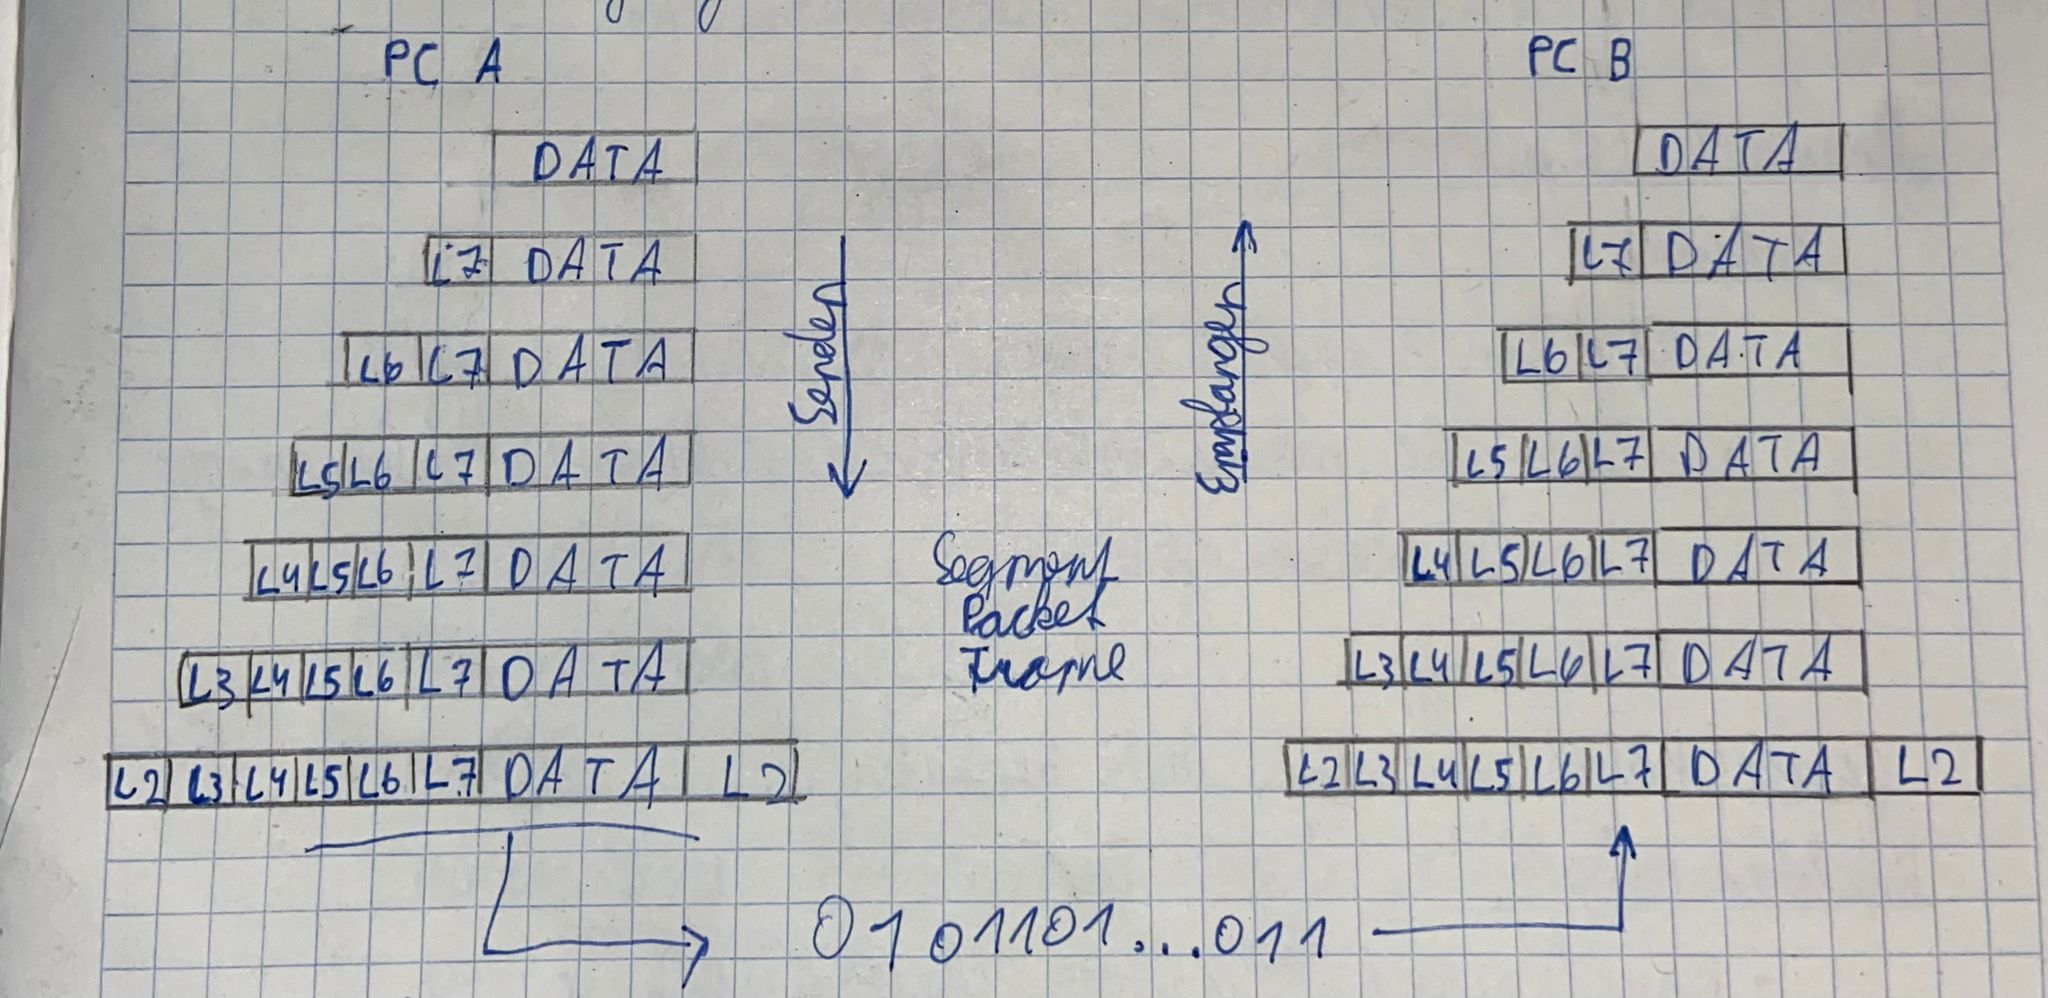
\includegraphics[width=0.9\linewidth]{figures/datenuber.jpeg}
	\caption{OSI-Modell Datenübertragung}
\end{figure}

\textbf{Layer 1 (Physical):} Bits übertragen \\
\textbf{Layer 2 (Data Link):} Lokale Adressierung, Fehlererkennung \\
\textbf{Layer 3 (Network):} Globale Adressierung, Routing \\
\textbf{Layer 4 (Transport):} Datenpaketzuordnung, Segmentierung, Datenfluss steuern \\
\textbf{Layer 5 (Session):} Session Verwalten, Verschlüsselung \\
\textbf{Layer 6 (Presentation):} Darstellung der Daten \\
\textbf{Layer 7 (Application):} Funktionen für die Application \\

%\subsection*{Cisco CLI}
%\begin{figure}[H]
%	\centering
%	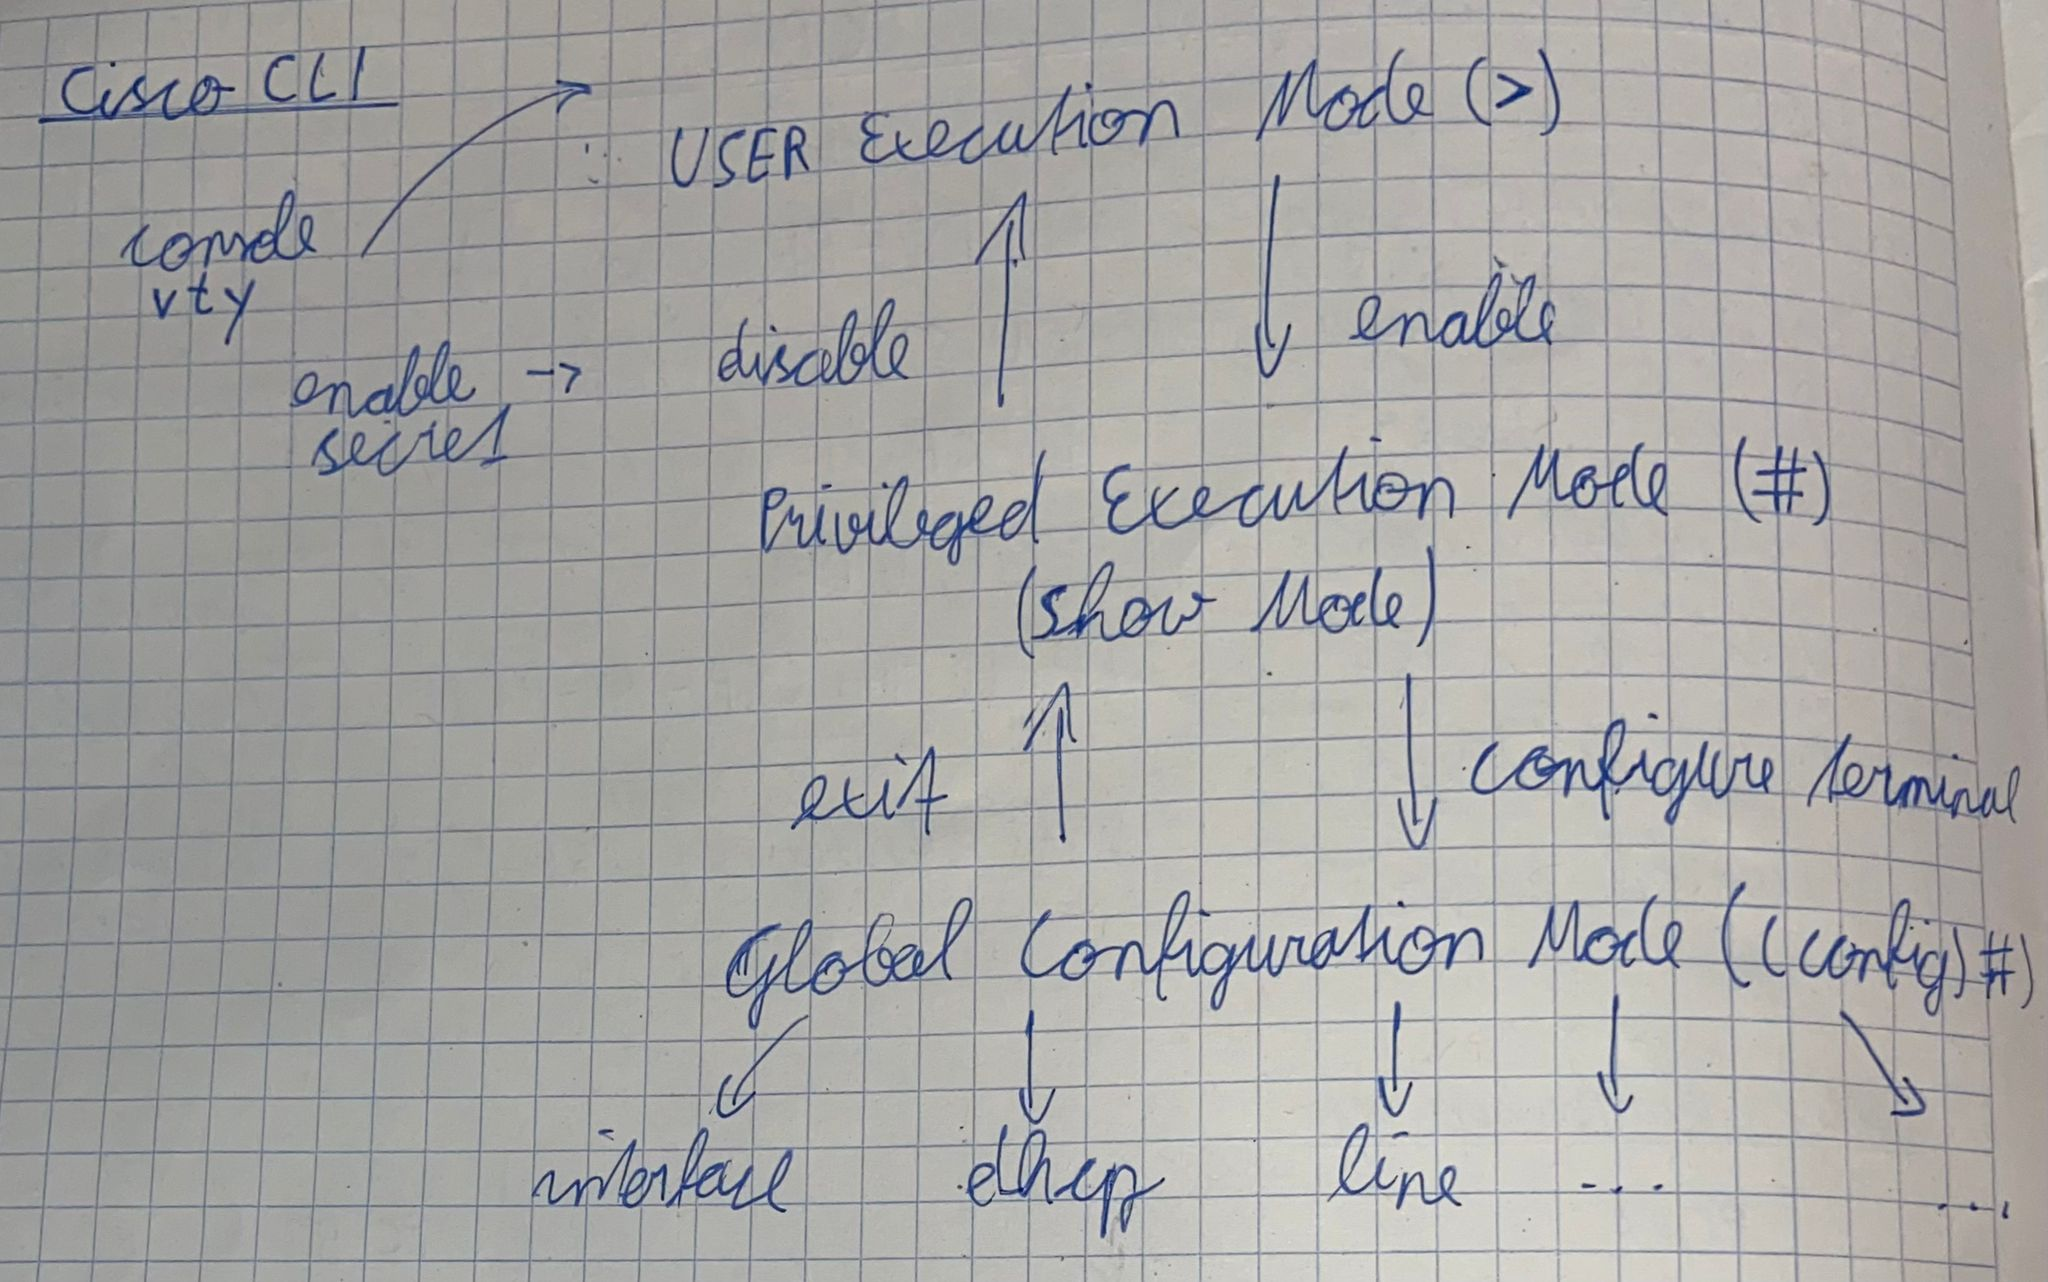
\includegraphics[width=0.9\linewidth]{figures/ciscocli.jpeg}
%	\caption{Cisco CLI}
%\end{figure}
	
	\subsection{Layer 1 (Physical)}
\subsection*{Aufgaben}
\begin{itemize}
	\item Bits von A nach B bringen
	\item elektrische, mechanische oder andere physische Verbindung zwischen zwei Geräten
	\item Kodierung
\end{itemize}
\textbf{Geräte:} Kabel, Antenne, Hub, Repeater,...

\subsection*{Wichtige Begriffe}
\begin{itemize}
	\item Bandbreite (bits/s $\rightarrow$ theoretisch)
	\item Durchsatz (bits/s $\rightarrow$ praktisch)
	\item Latenz (Dauer der Daten von A bis B in ms)
\end{itemize}

\subsection*{Typische Medien}
\begin{itemize}
	\item Kupferkabel (Twisted-Pair-Kabel)
	\item[] \begin{tabbing}
		+ Günstig ~~~~~~~~~~~~~~~~~~~~~ \= $\approx$ Distanz (ca 100m) \\
		+ einfache Handhabung ~~~~ \= $\approx$ Geschwindigkeit \\
		~~~~~~~~~~~~~~~~~~~~~~~~~~~~~~~~~~~~ \= - Interferenzen (Störungen)
	\end{tabbing}
	\begin{itemize}
		\item Straight Through (beide Enden gleich)	
		\item Crossover (verschiedene Enden)
	\end{itemize}
	\item[] (durch Auto MDIX werden Enden automatisch konfiguriert)
	\item Koaxialkabel
	\item Glasfaserkabel
	\begin{tabbing}
		Arten: ~~ \= Single-Mode (Senden Laser, Reichweite 1-10km) \\
		~~~~~~~~~~~ \= Multi-Mode (Senden LED, Reichweite ca 600m)
	\end{tabbing}
	\item[] \begin{figure}[H]
		\centering
		\subfloat[\centering Single-Mode]{{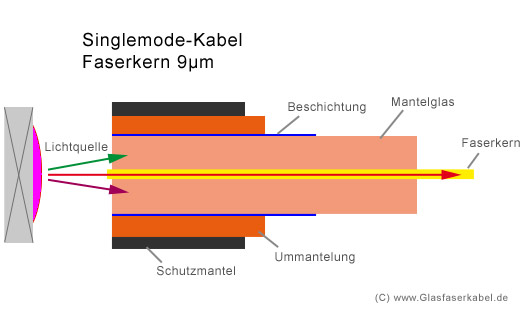
\includegraphics[width=0.46\linewidth]{figures/singlemode.jpg} }}
		\qquad
		\subfloat[\centering Multi-Mode]{{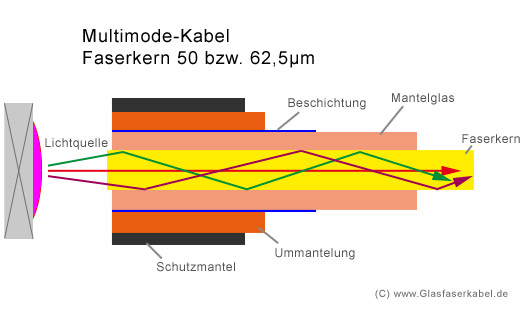
\includegraphics[width=0.46\linewidth]{figures/multimode.jpg} }}
		\caption{Glasfaserkabelarten}
	\end{figure}
	\item[] \begin{tabbing}
		+ Speed ~~~~~~~~~~~~~~~~~ \= - Teuer \\
		+ Reichweite ~~~~~~~~~~~ \= - Handhabung \\
		+ Störungen
	\end{tabbing}
	\item Drahtlos
	\item[] Übertragung: elektromagnetische Wellen über Luft
	\item[] \begin{tabbing}
		+ Flexibel ~~~ \= - Störungen \\
		~~~~~~~~~~~~~~~~~ \= - Shared Medium \\
		~~~~~~~~~~~~~~~~~ \= - Reichweite (ca 100m), Hindernisse \\
		~~~~~~~~~~~~~~~~~ \= - Security \\
	\end{tabbing}
\end{itemize}
	\subsection{Layer 2 (Data Link)}
\subsection*{Aufgaben}
\begin{itemize}
	\item lokale Adressierung
	\item Fehlererkennung
	\item Zugang zum Medium herstellen
	\item Kommunikation mit Layer 3
\end{itemize}

\textbf{Geräte:} Netzwerkkarte, Switch, Bridge,... \\
\textbf{Standards:} Wifi (802.11), Ethernet (802.2, 802.3)
\subsection*{Topologie}
\begin{itemize}
	\item Sterntopologie
	\item Baumtopologie
	\item Punkt-zu-Punkt
\end{itemize}
\begin{figure}[H]
	\centering
	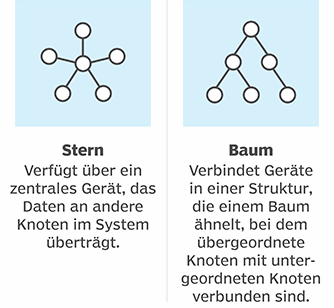
\includegraphics[width=0.6\linewidth]{figures/topologiearten.png}
	\caption{Baum- und Sterntopologie}
\end{figure}

\subsection*{Ethernet}
\begin{figure}[H]
	\centering
	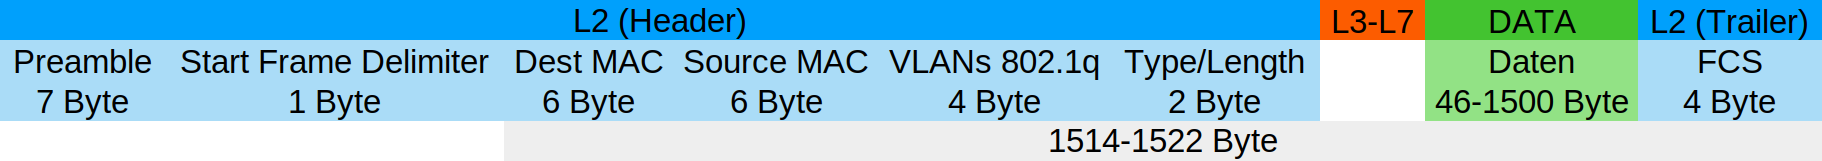
\includegraphics[width=1.0\linewidth]{figures/ethheader.png}
	\caption{Ethernet Frame}
\end{figure}

\subsection*{MAC-Adresse}
Die MAC-Adresse ist eine 48-Bit Zahl und wird in hexadecimal dargestellt.
\begin{tabbing}
	Bsp:\\
	Hersteller ~ \= für den Hersteller einzigartig \\
	DC F5 05 $\vert$\= 17 9A 69 \\
\end{tabbing}

Jede Netzwerkkarte besitzt eine weltweit einzigartige (theoretisch) MAC-Adresse.

\subsection*{Type}
Kodierung für Layer 3 \\
0x800 $\rightarrow$ IP \\
0x806 $\rightarrow$ ARP 

\subsection*{Fehlerkennung}
Frame Checksum (CRC) \\
Polynomdivision mit einem Polynom von Grad 32

\subsection*{Funktion eines Switches}
Der Switch baut mit der Source-MAC seine MAC-Tabelle auf. Dort steht zu jeder MAC-Adresse der passende Port. Falls die MAC-Adresse schon eingetragen ist, wird ein Timer aktualisiert. Sollte es noch keinen Eintrag geben wird er hinzugefügt und bleibt dort eine gewisse Zeit (5 Minuten) bevor er gelöscht wird. Der Switch vergleicht die Destination-MAC mit seiner MAC-Tabelle. Falls der Switch keinen Eintrag findet sendet er an alle Ports (Flooding, Unknown Unicast). Sonst sendet er an den Port, wo er den Frame bekommen hat. \\
Layer 2 Broadcast Adresse: FF:FF:FF:FF:FF:FF

\subsection*{L2, L3 Adressierung}
\begin{figure}[H]
	\centering
	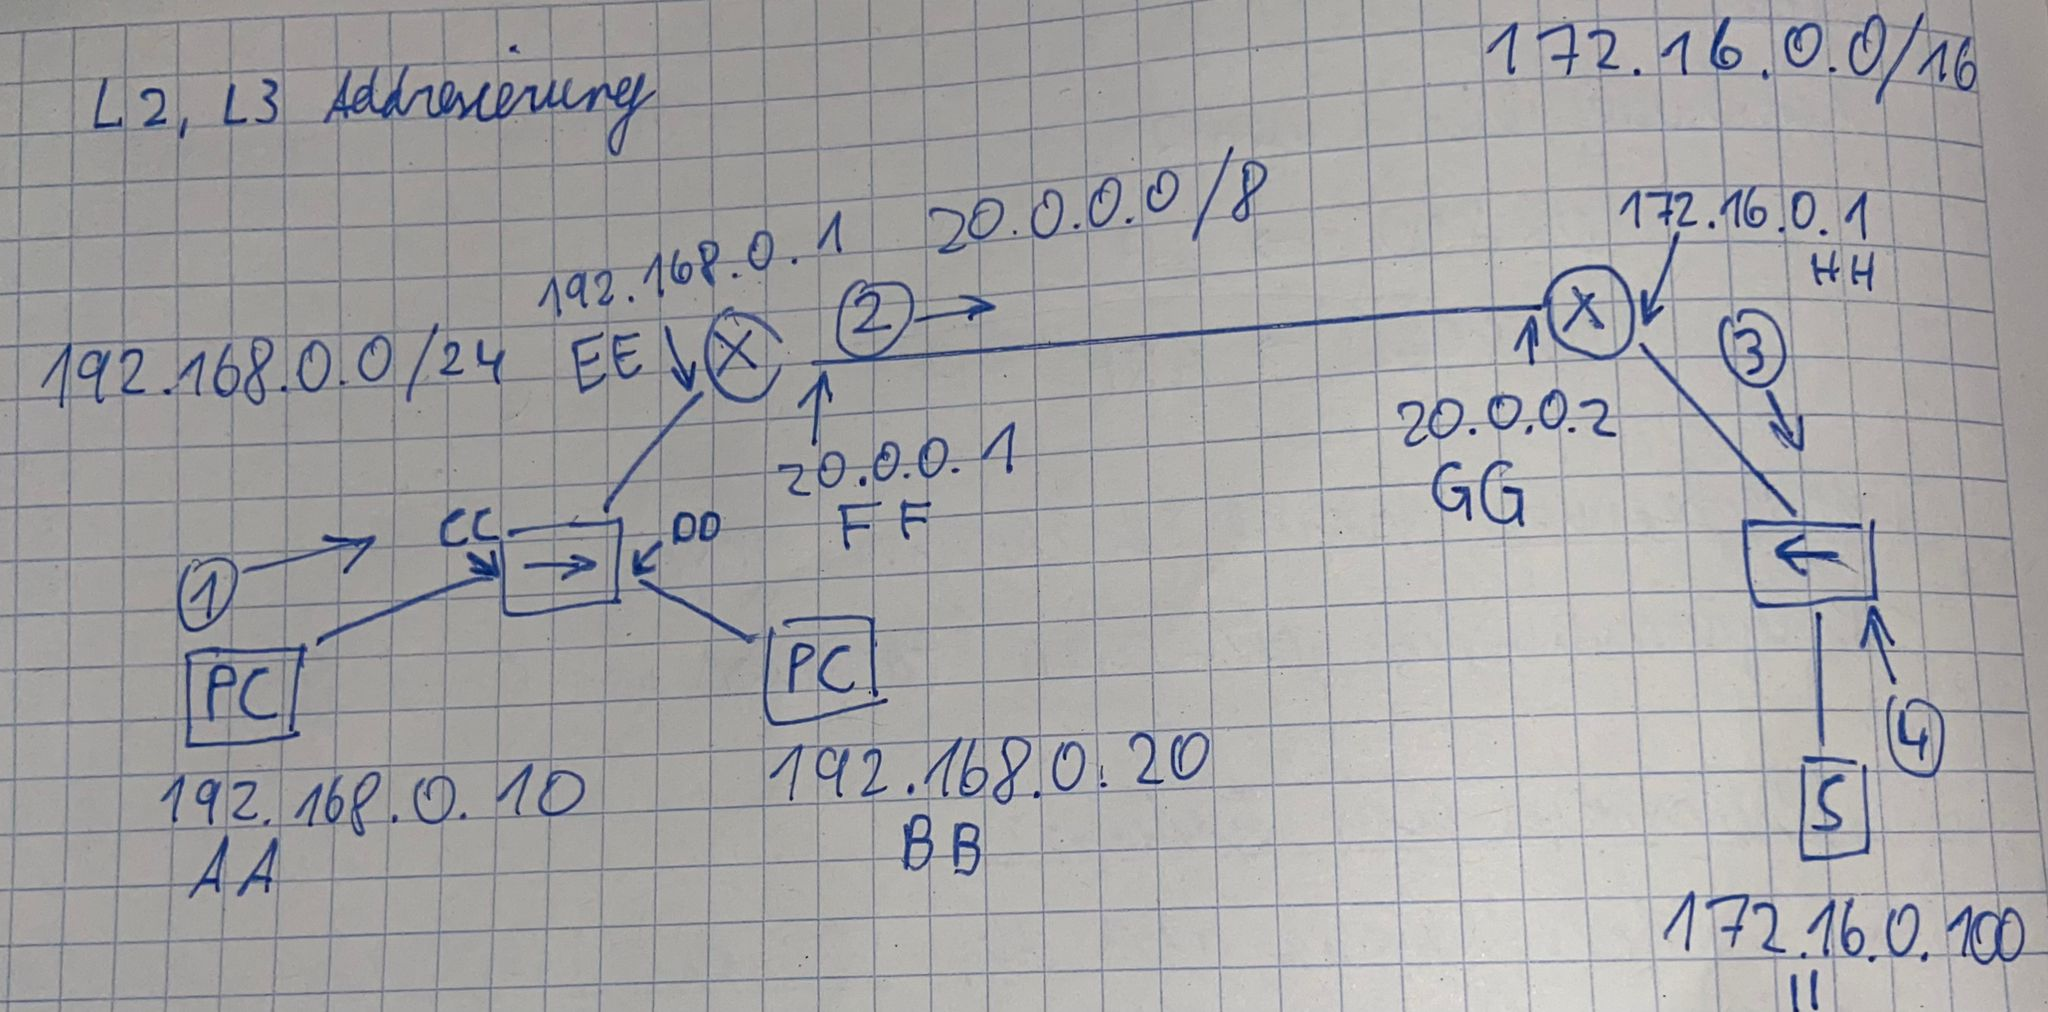
\includegraphics[width=1.0\linewidth]{figures/l2l3add.jpeg}
	\caption{Layer 2 \& 3 Adressierung}
\end{figure}

\begin{table}[H]
	\begin{tabular}{c|cccc}
		& Source MAC & Destination MAC & Source IP & Destination IP \\
		\hline
		1 & AA & EE & 192.168.0.10 & 172.16.0.100 \\
		2 & FF & GG & 192.168.0.10 & 172.16.0.100 \\
		3 & HH & II & 192.168.0.10 & 172.16.0.100 \\
		4 & II & HH & 172.16.0.100 & 192.168.0.10
	\end{tabular}
\end{table}

\subsection*{ARP (Address Resolution Protocol)}
Nutzt ein Host um zu einer gegebenen IP-Adresse die passende MAC-Adresse zu finden

\subsubsection*{ARP-Request (Broadcast)}
Source MAC: eigene MAC-Adresse \\
Destination MAC: FF-FF-FF-FF-FF-FF \\
Type: 0x806
Danach ARP-Header (IP, MAC, Protokoll)

\subsubsection*{ARP-Reply}
Unicast (auch als Broadcast möglich) \\
Source MAC: eigene MAC-Adresse (gesucht) \\
Destination MAC: MAC-Adresse (Anfrage) \\
Type: 0x806 \\
Danach ARP-Header

\subsubsection*{ARP-Cache}
Die Einträge werden im ARP-Cache gespeichert (ca 5 min) \\
IP MAC Time

\subsection*{ARP-Spoofing}
\begin{figure}[H]
	\centering
	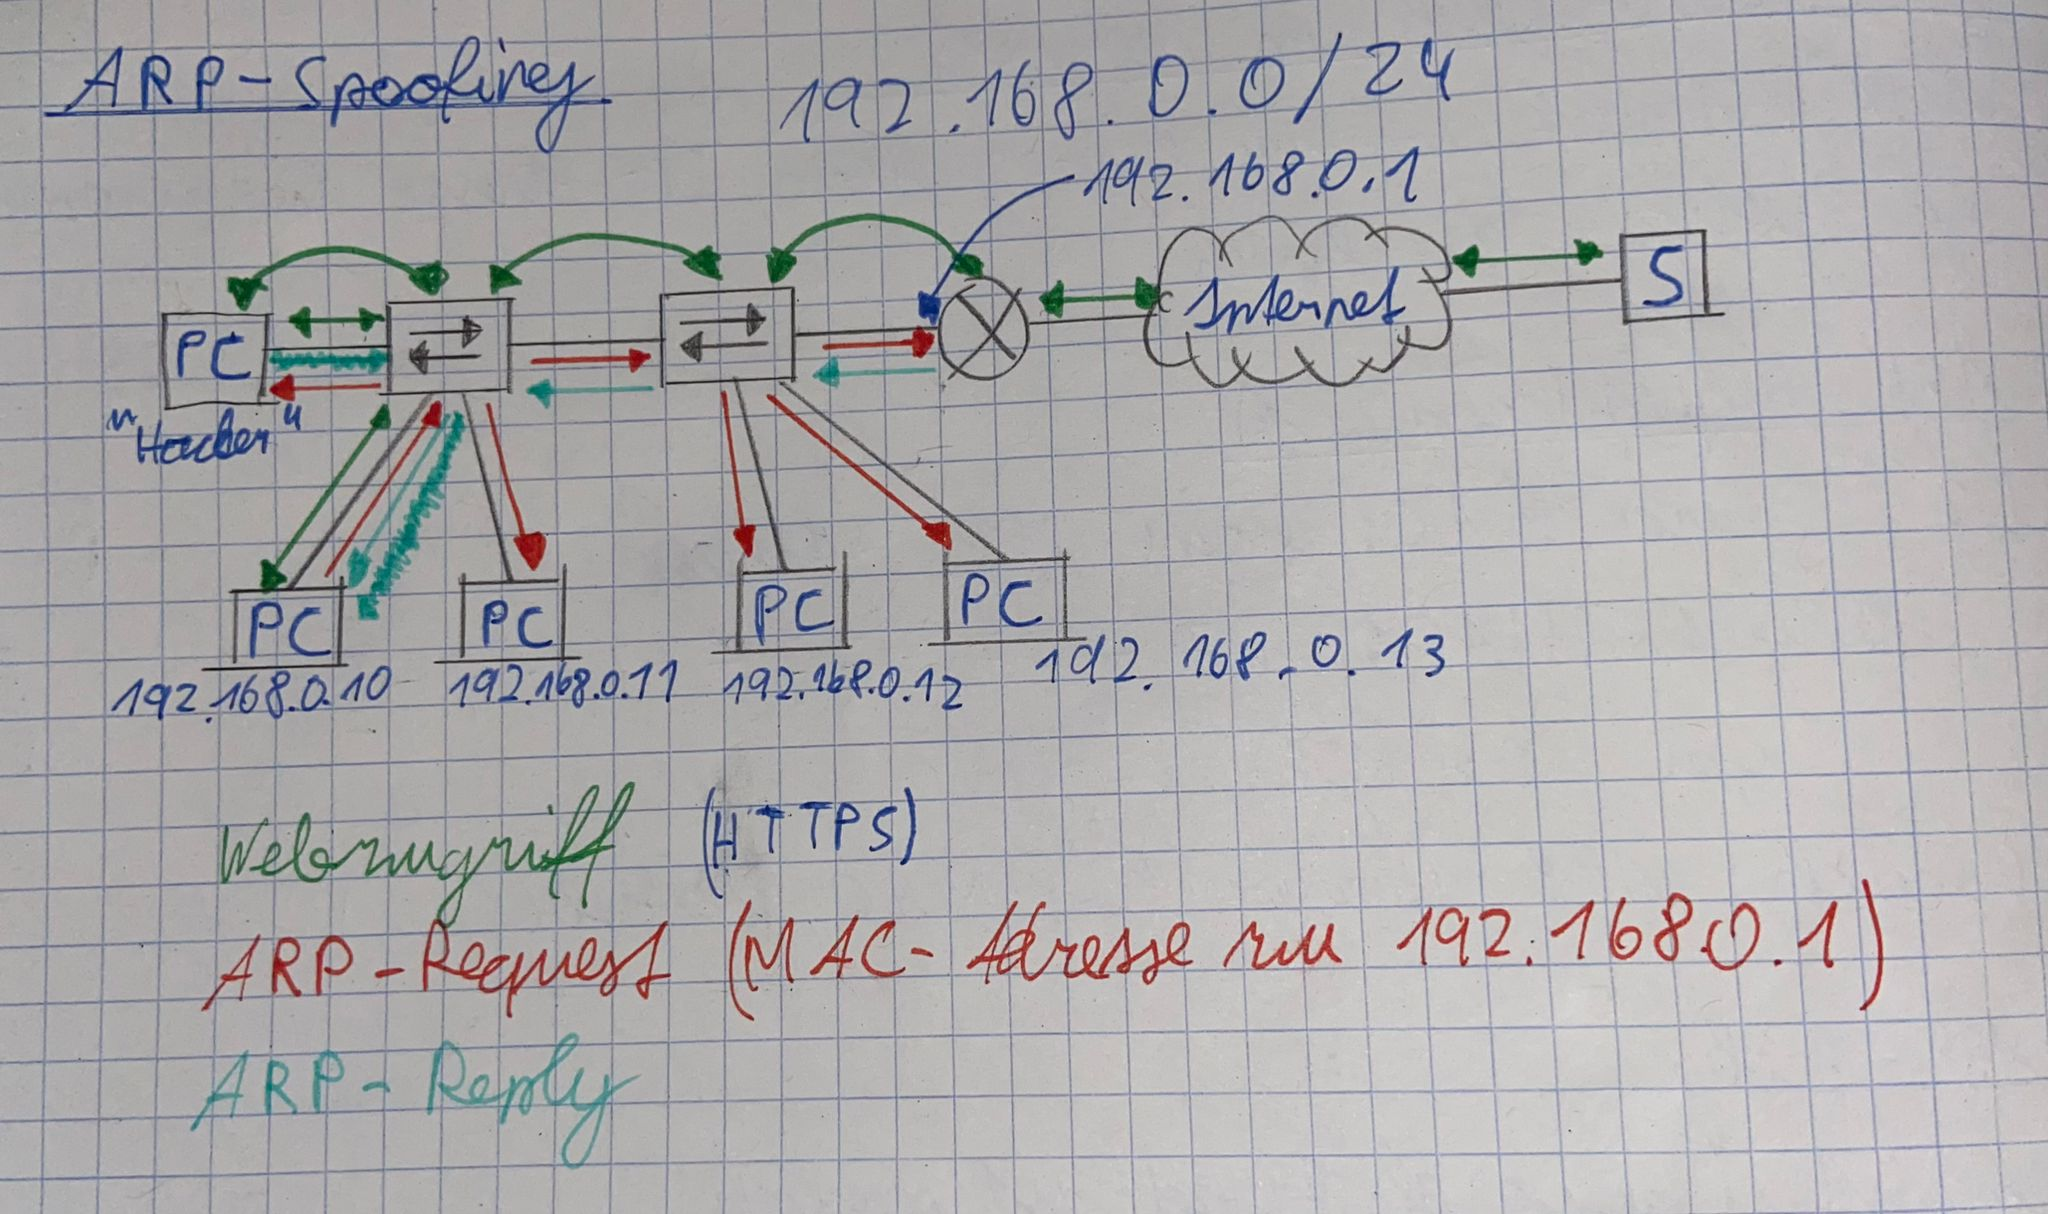
\includegraphics[width=1.0\linewidth]{figures/arpspoofing.jpeg}
	\caption{ARP-Spoofing}
\end{figure}






	\subsection{Layer 3 (Network)}
\subsection*{Aufgaben}
\begin{itemize}
	\item Routing
	\item Globale Adressierung
	\item Kommunikation mit L2 \& L4
\end{itemize}
\textbf{Protkolle:} IPv4, IPv6, ICMP, RIP, OSPF, EIGRP, IS-IS, BGP

\subsection*{IPv4}
Eigenschaften von IP
\begin{itemize}
	\item Verbindungslos
	\item Best Effort
	\item Medium unabhängig
\end{itemize}
\textbf{IP-Header (8.2.2)}
Wichtige Felder: Source \& Destination IP, Time-to-Live

\subsection*{Kommunikationsart}
\begin{itemize}
	\item Unicast (IP des Host)
	\item Multicast (224.0.0.0 - 239.255.255.255)
	\item Broadcast (letzte IP im Netz, 255.255.255.255)
\end{itemize}

\subsection*{Spezielle IP-Adressen}
\begin{itemize}
	\item 127.0.0.0 / 8 ... localhost
	\item 10.0.0.0 / 8
	\item[] 172.16.0.0 / 12
	\item[] 192.168.0.0 / 16 ... private IP-Adressen (NAT)
	\item 169.254.0.0 / 16 ... APIPA
	\item 192.0.2.0 / 24 ... Testnetz
\end{itemize}
\textbf{Fazit:} Zu wenig IPv4-Adressen!

\subsection*{Deshalb}
\begin{itemize}
	\item VLSM (variable length subnet mask)
	\item NAT
	\item IPv6
\end{itemize} 

\subsection*{Classful Addressing (uralt)}
Das erste Oktett bestimmt die Subnetzmaske (/8, /16, /24)
\begin{table}[H]
	\begin{tabular}{ccll}
		Klasse A & 0-127 & (0...) & /8 \\
		Klasse B & 128-191 & (10...) & /16 \\
		Klasse C & 192-223 & (110...) & /24 \\
		Klasse D & 224-239 & (1110...) & Multicast \\
		Klasse E & 240-255 & (11110...) & für spätere Verwendung
	\end{tabular}
\end{table}

\subsection*{Classless Addressing (veraltet!)}
Die Subnetzmasken /8, /16, /24 können beliebig verwendet werden

\subsection*{CIDR (Classless Inter-Domain Routing)}
Es können beliebige Subnetzmasken (z.B. /25, /26, ...) verwendet werden. Alle Subnetze werden gleich groß.

\subsection*{VLSM (variable length subnet mask)}
Alle Subnetzmasken können beliebig verwendet werden. Die Netzte dürfen sich nicht überschneiden.

\subsection*{Subnetzmasken}
\begin{table}[H]
	\begin{tabular}{cccl}
		Präfix Notation & Dotted Decimal Notation & Hosts & Subnetz von /24 \\
		/25 & 255.255.255.128 & $2^{7}$ - 2 = 126 & 2 \\
		/26 & 255.255.255.192 & $2^{6}$ - 2 = 62 & 4 \\
		/27 & 255.255.255.224 & $2^{5}$ - 2 = 30 & 8 \\
		/28 & 255.255.255.240 & $2^{4}$ - 2 = 14 & 16 \\
		/29 & 255.255.255.248 & $2^{3}$ - 2 = 6 & 32 \\
		/30 & 255.255.255.252 & $2^{2}$ - 2 = 2 & 64 \\
		/31 & 255.255.255.254 & $2^{1}$ - 2 = 0 & für spezielle Anwendung \\
		/20 & 255.255.240.0 & $2^{12}$ - 2 = 4.094 & /
	\end{tabular}
\end{table}

\subsection*{Bsp 1 (CIDR):}
\begin{figure}[H]
	\centering
	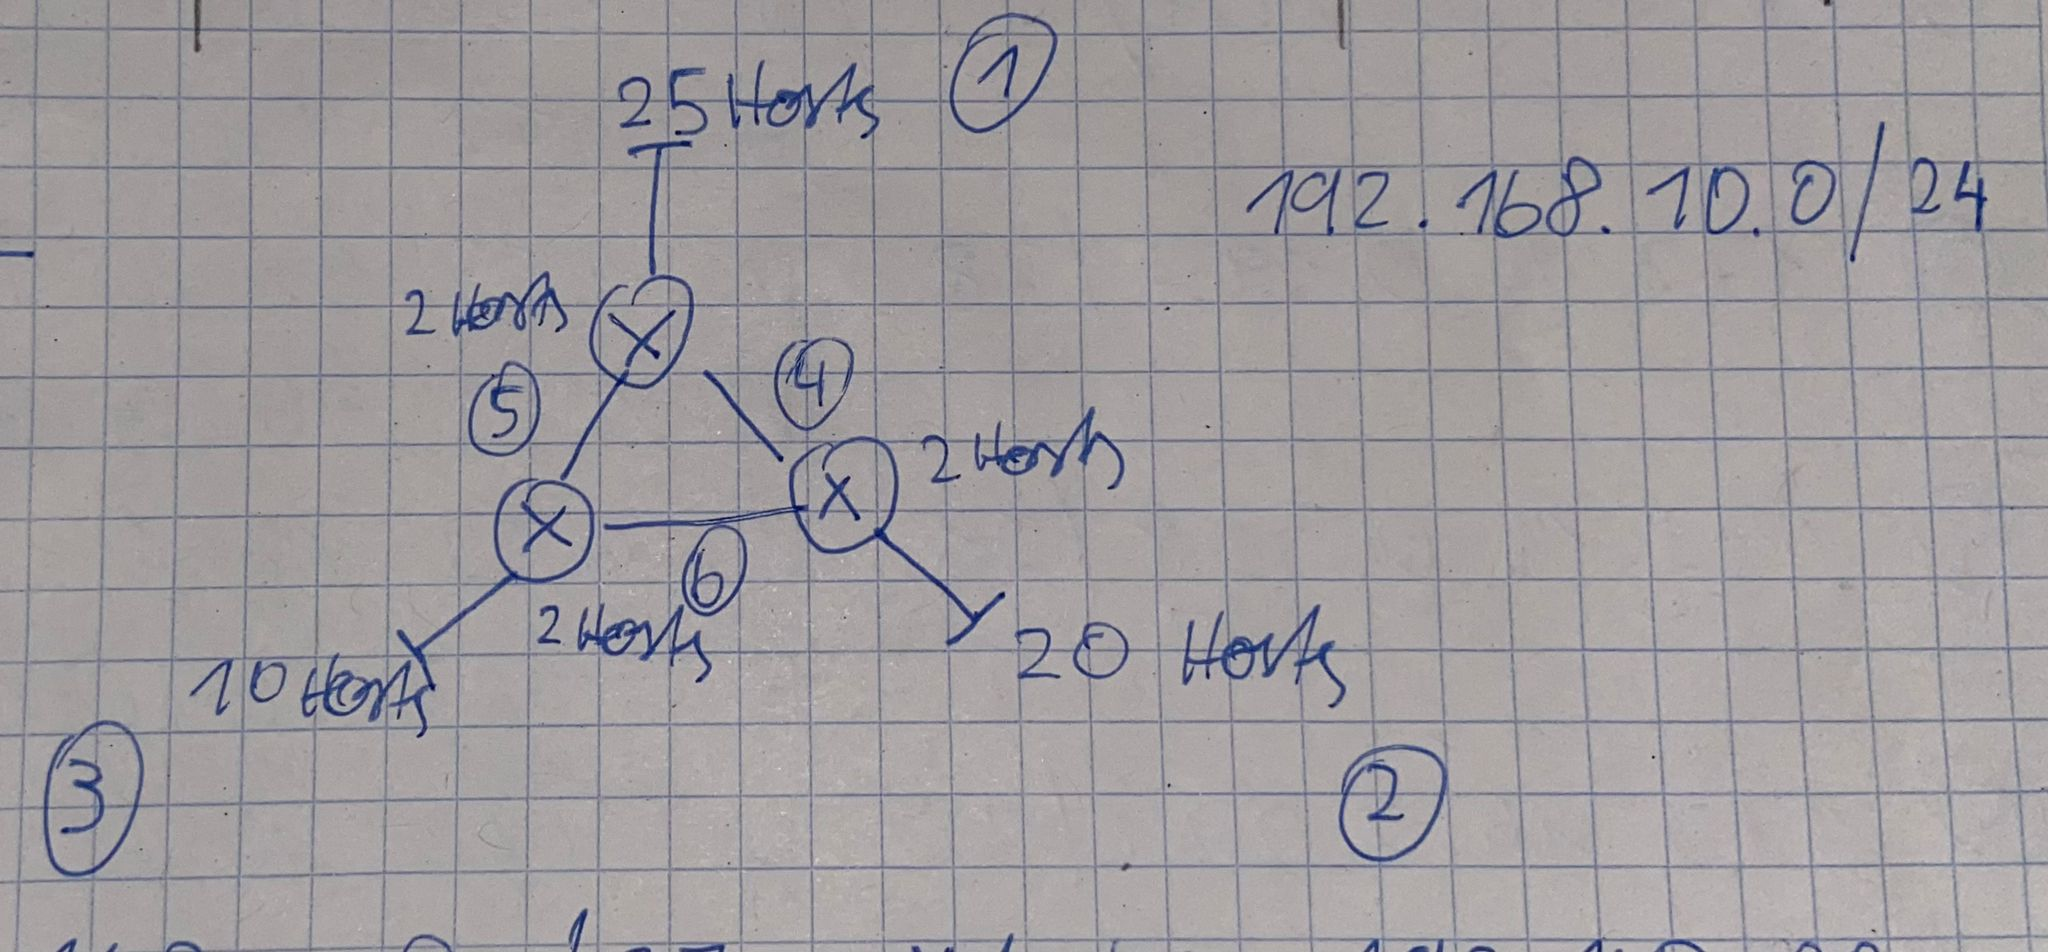
\includegraphics[width=1.0\linewidth]{figures/bsp1_cidr.jpeg}
	\caption{CIDR Beispiel}
\end{figure}
\begin{table}[H]
	\begin{tabular}{llll}
		1 & 192.168.10.0 / 27 & Netzadresse & 192.168.100.0 \\
		&  & Broadcast & 192.168.100.31 \\
		\hline
		2 & 192.168.10.32 / 27 & Netzadresse & 192.168.100.32 \\
		&  & Broadcast & 192.168.100.63 \\
		\hline
		3 & 192.168.10.64 / 27 & Netzadresse & 192.168.100.64 \\
		&  & Broadcast & 192.168.100.95 \\
		\hline
		4 & 192.168.10.96 / 27 & Netzadresse & 192.168.100.96 \\
		&  & Broadcast & 192.168.100.127 \\
		\hline
		5 & 192.168.10.128 / 27 & Netzadresse & 192.168.100.128 \\
		&  & Broadcast & 192.168.100.159 \\
		\hline
		6 & 192.168.10.160 / 27 & Netzadresse & 192.168.100.160 \\
		&  & Broadcast & 192.168.100.191
	\end{tabular}
\end{table}

\subsection*{Bsp 2 (VLSM):}
\begin{figure}[H]
	\centering
	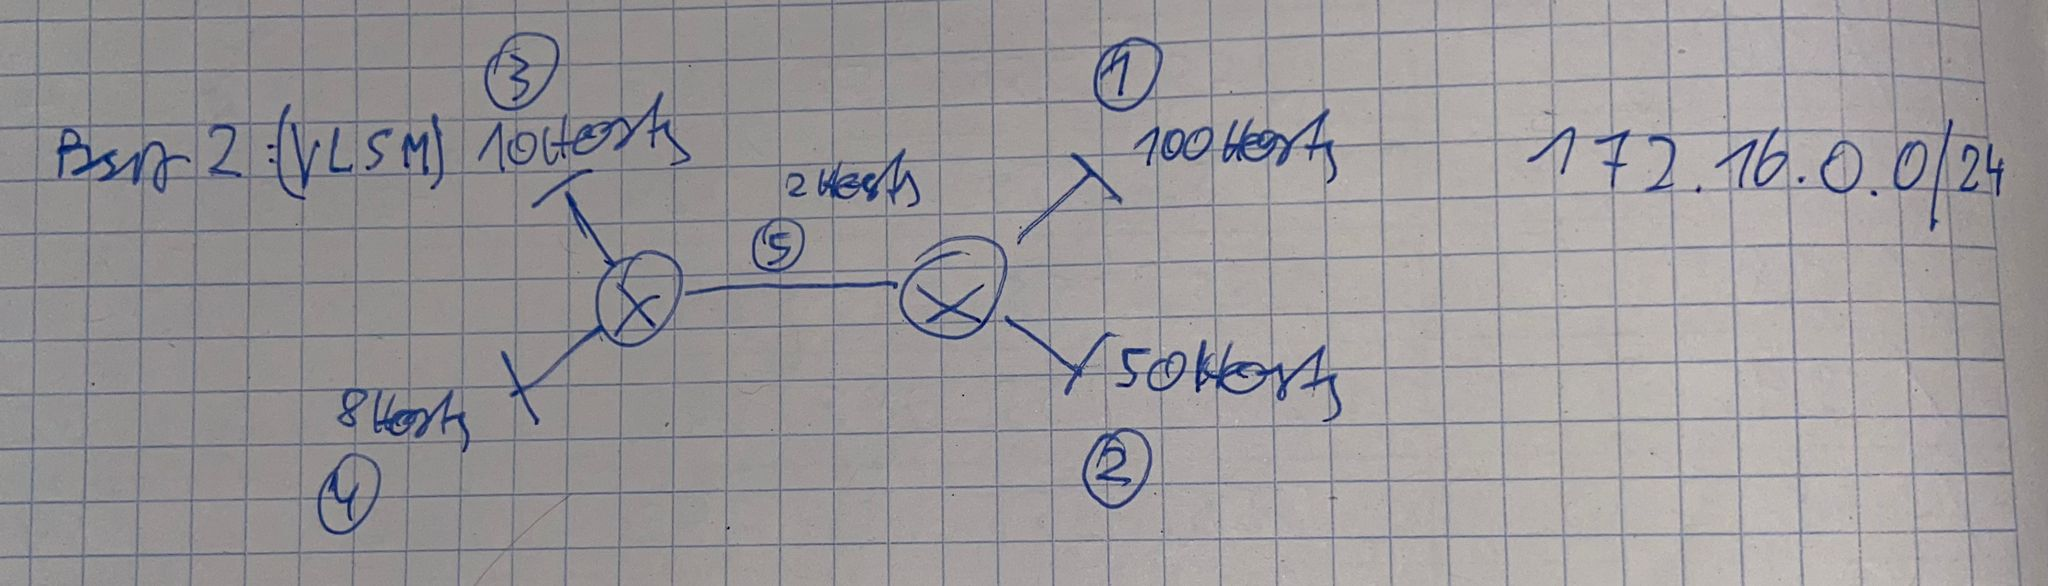
\includegraphics[width=1.0\linewidth]{figures/bsp2_vlsm.jpeg}
	\caption{VLSM Beispiel}
\end{figure}
\begin{table}[H]
	\begin{tabular}{llll}
		1 & 172.16.0.0 / 25 & Netzadresse & 172.16.0.0 \\
		&  & Broadcast & 172.16.0.127 \\
		\hline
		2 & 172.16.0.128 / 26 & Netzadresse & 172.16.0.128 \\
		&  & Broadcast & 172.16.0.191 \\
		\hline
		3 & 172.16.0.192 / 28 & Netzadresse & 172.16.0.192 \\
		&  & Broadcast & 172.16.0.207 \\
		\hline
		4 & 172.16.0.208 / 28 & Netzadresse & 172.16.0.208 \\
		&  & Broadcast & 172.16.0.223 \\
		\hline
		5 & 172.16.0.224 / 30 & Netzadresse & 172.16.0.224 \\
		&  & Broadcast & 172.16.0.227
	\end{tabular}
\end{table}

(PT: 10.4.3, 11.5.5, 11.9.3, 11.10.1)







	\subsection{Layer 4 (Transport)}
\textbf{Aufgaben}
\begin{itemize}
	\item Anwendungen identifizieren
	\item Segmentierung
	\item ev. Flusskontrolle, Verbindungsauf- \& abbau
	\item Kommunikation mit L3 \& L5
\end{itemize}

\textbf{Protkolle:} 
\begin{itemize}
	\item TCP (Transmission Control Protocol)
	\item UDP (User Datagram Protocol)
\end{itemize}

\begin{table}[H]
	\begin{tabular}{l|l}
		\multicolumn{1}{c|}{TCP} & \multicolumn{1}{c}{UDP} \\
		\hline
		Anwendungen identifizieren (Ports) & Anwendungen identifizieren (Ports) \\
		Segmentierung & Segmentierung \\
		Verbindungen auf- bzw abbauen &  \\
		Segmente ordnen &  \\
		wiederholtes Senden &  \\
		Flusskontrolle & 
	\end{tabular}
\end{table}

TCP: HTTP (80)/HTTPS (443), SMTP (25), POP (110), IMAP (143), Telnet (23), SSH (22), FTP (20/21),... \\
UDP: DNS (53), DHCP (67/68), VoIP, Streaming,...

\textbf{Ports} \\
Der Port ist eine 16-Bit Zahl $\rightarrow$ $2^{16} = 65.536$ \\
Der Port identifiziert die Anwendung, sowohl beim Server als auch beim Client.

\textbf{Gruppe von Ports}
\begin{table}[H]
	\begin{tabular}{rc}
		Well-Known-Ports & 0 - 1.023 \\
		Registered-Ports & 1.024 - 49.151 \\
		Private Ports & 49.152 - 65.535
	\end{tabular}
\end{table}

\textbf{L4-Adressierung}
\begin{figure}[H]
	\centering
	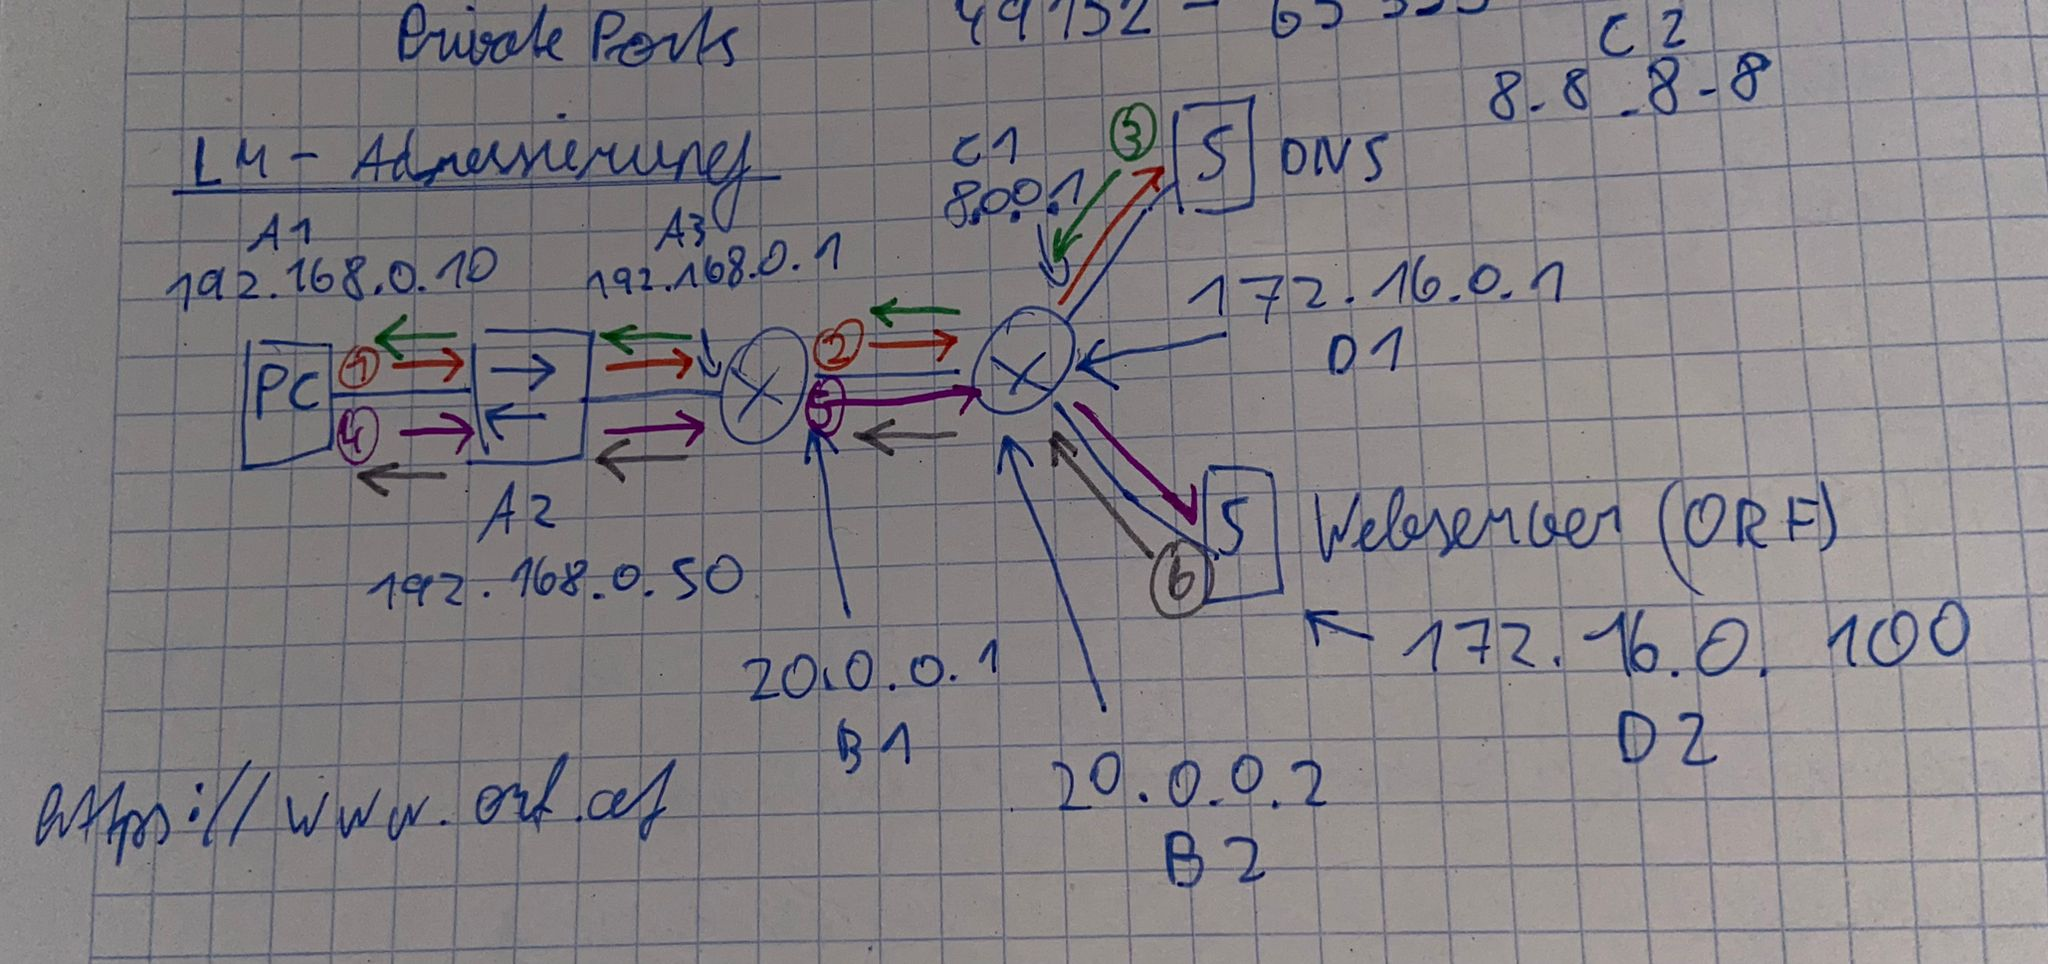
\includegraphics[width=1.0\linewidth]{figures/l4_addr.jpeg}
	\caption{L4-Adressierung}
	\label{fig:l4_addr}
\end{figure}

\begin{table}[H]
	\begin{tabular}{c|ccllll}
		& \multicolumn{2}{c}{L2 (MAC)} & \multicolumn{2}{c}{L3 (IP)} & \multicolumn{2}{c}{L4 (Ports)} \\
		& \multicolumn{1}{c}{Source} & \multicolumn{1}{c}{Destination} & \multicolumn{1}{c}{Source} & \multicolumn{1}{c}{Destination} & \multicolumn{1}{c}{Source} & \multicolumn{1}{c}{Destination} \\
		\hline
		1 & A1 & A3 & 192.168.0.10 & 8.8.8.8 & 53.722 & 53 \\
		2 & B1 & B2 & 192.168.0.10 & 8.8.8.8 & 53.722 & 53 \\
		3 & C2 & C1 & 8.8.8.8 & 192.168.0.10 & 53 & 53.722 \\
		4 & A1 & A3 & 192.168.0.10 & 172.16.0.100 & 60.112 & 443 \\
		5 & B1 & B2 & 192.168.0.10 & 172.16.0.100 & 60.112 & 443 \\
		6 & D2 & D1 & 172.16.0.100 & 192.168.0.10 & 443 & 60.112
	\end{tabular}
\end{table}

\textbf{TCP} \\
Verbindungsaufbau: Drei-Wege-Handshake
\begin{figure}[H]
	\centering
	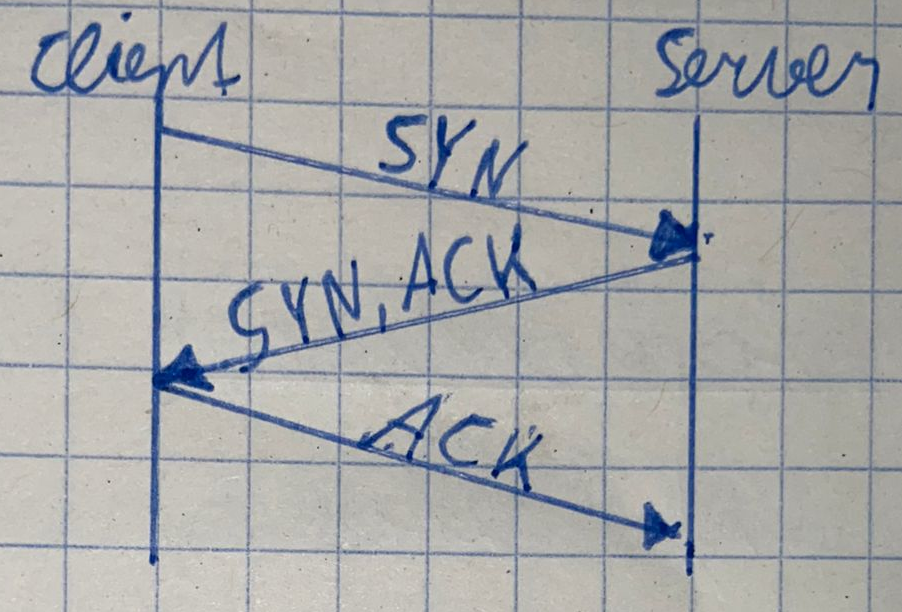
\includegraphics[width=0.8\linewidth]{figures/tcp_3wh.png}
	\caption{TCP 3-Way-Handshake}
\end{figure}

Verbindungsabbau: Zwei-Wege-Handshake
\begin{figure}[H]
	\centering
	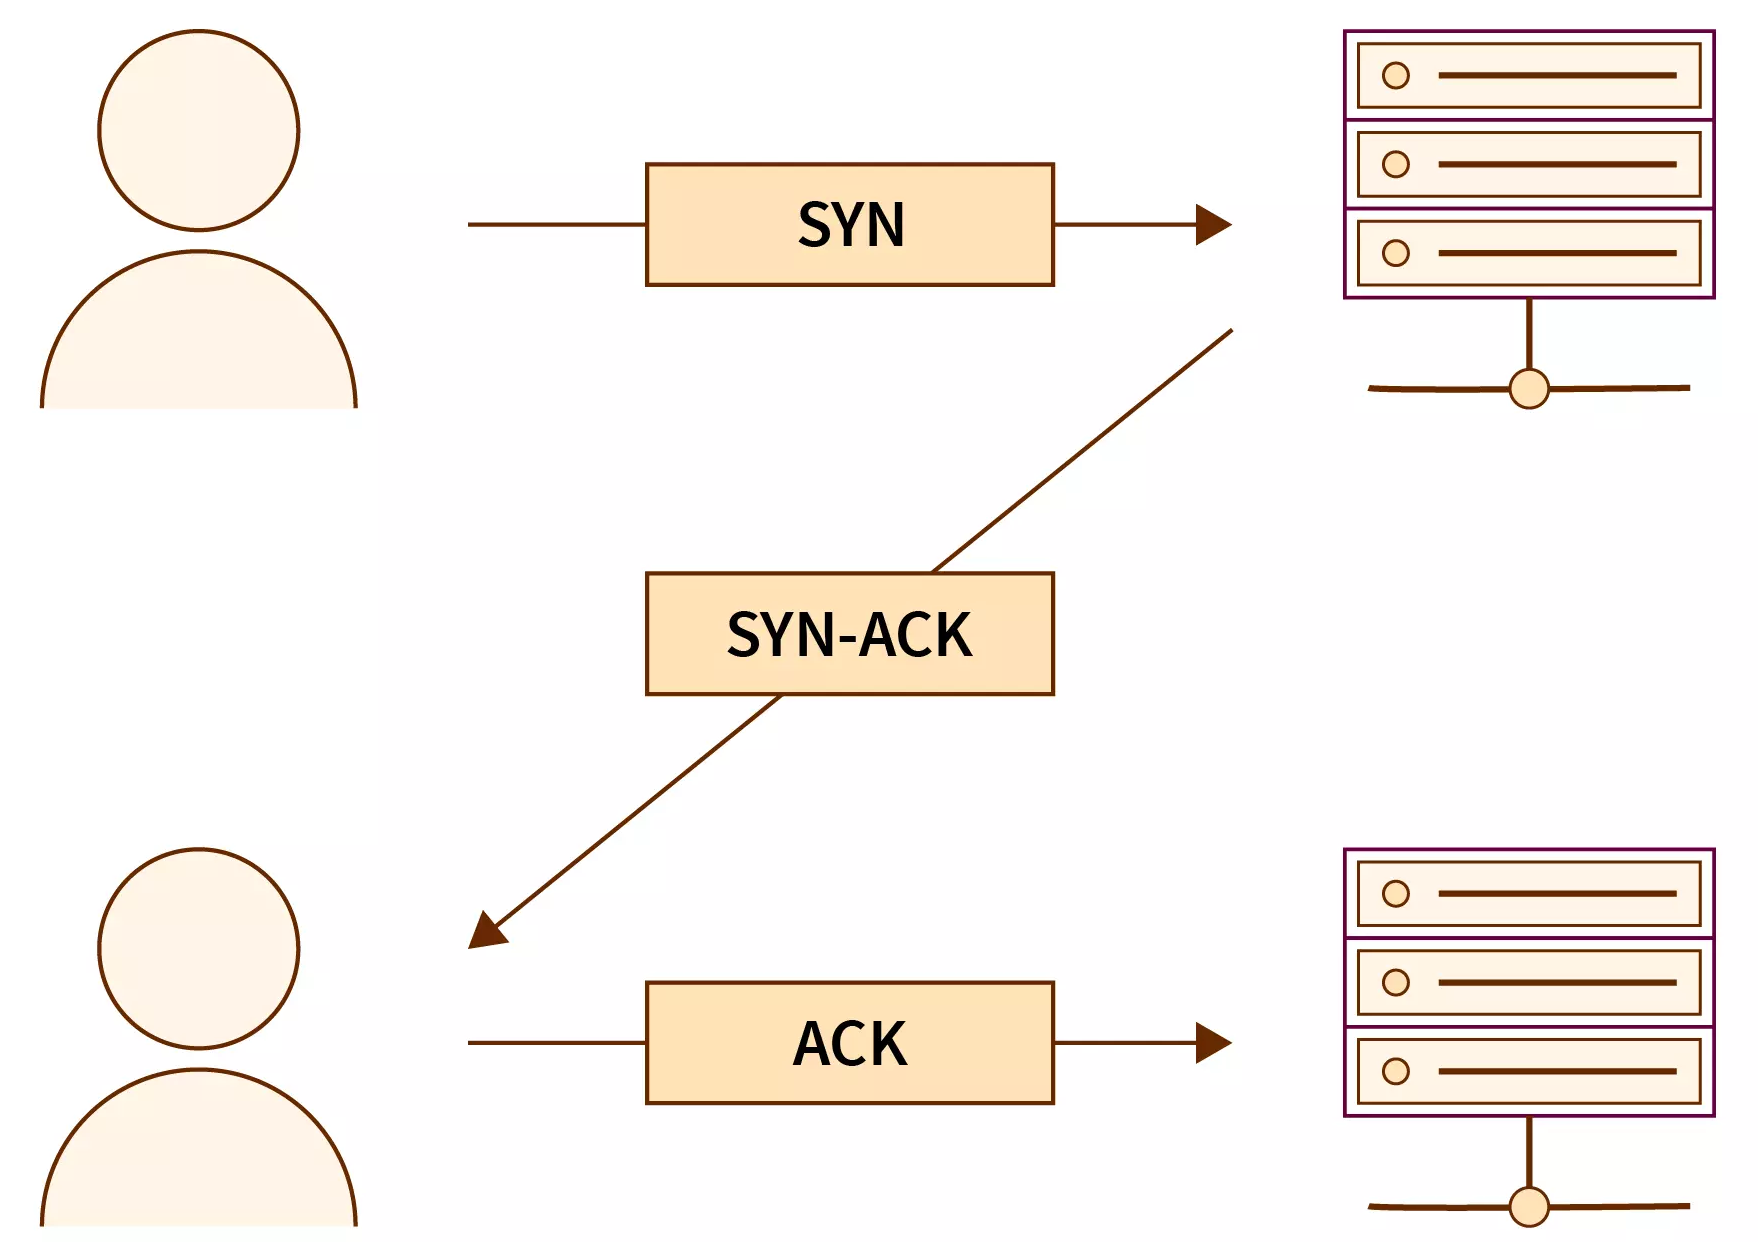
\includegraphics[width=0.8\linewidth]{figures/tcp_2wh.png}
	\caption{TCP 2-Way-Handshake}
\end{figure}

\textbf{Segmentierung} \\
Es wird eine SEQUENCENUMBER mitgeschickt. Diese gibt die Reihenfolge an. Der Client bestätigt die Segmente mit ACK-Segmente. Die ACK-NUMBER gibt an, welches Segment als nächstes kommen soll.
\begin{figure}[H]
	\centering
	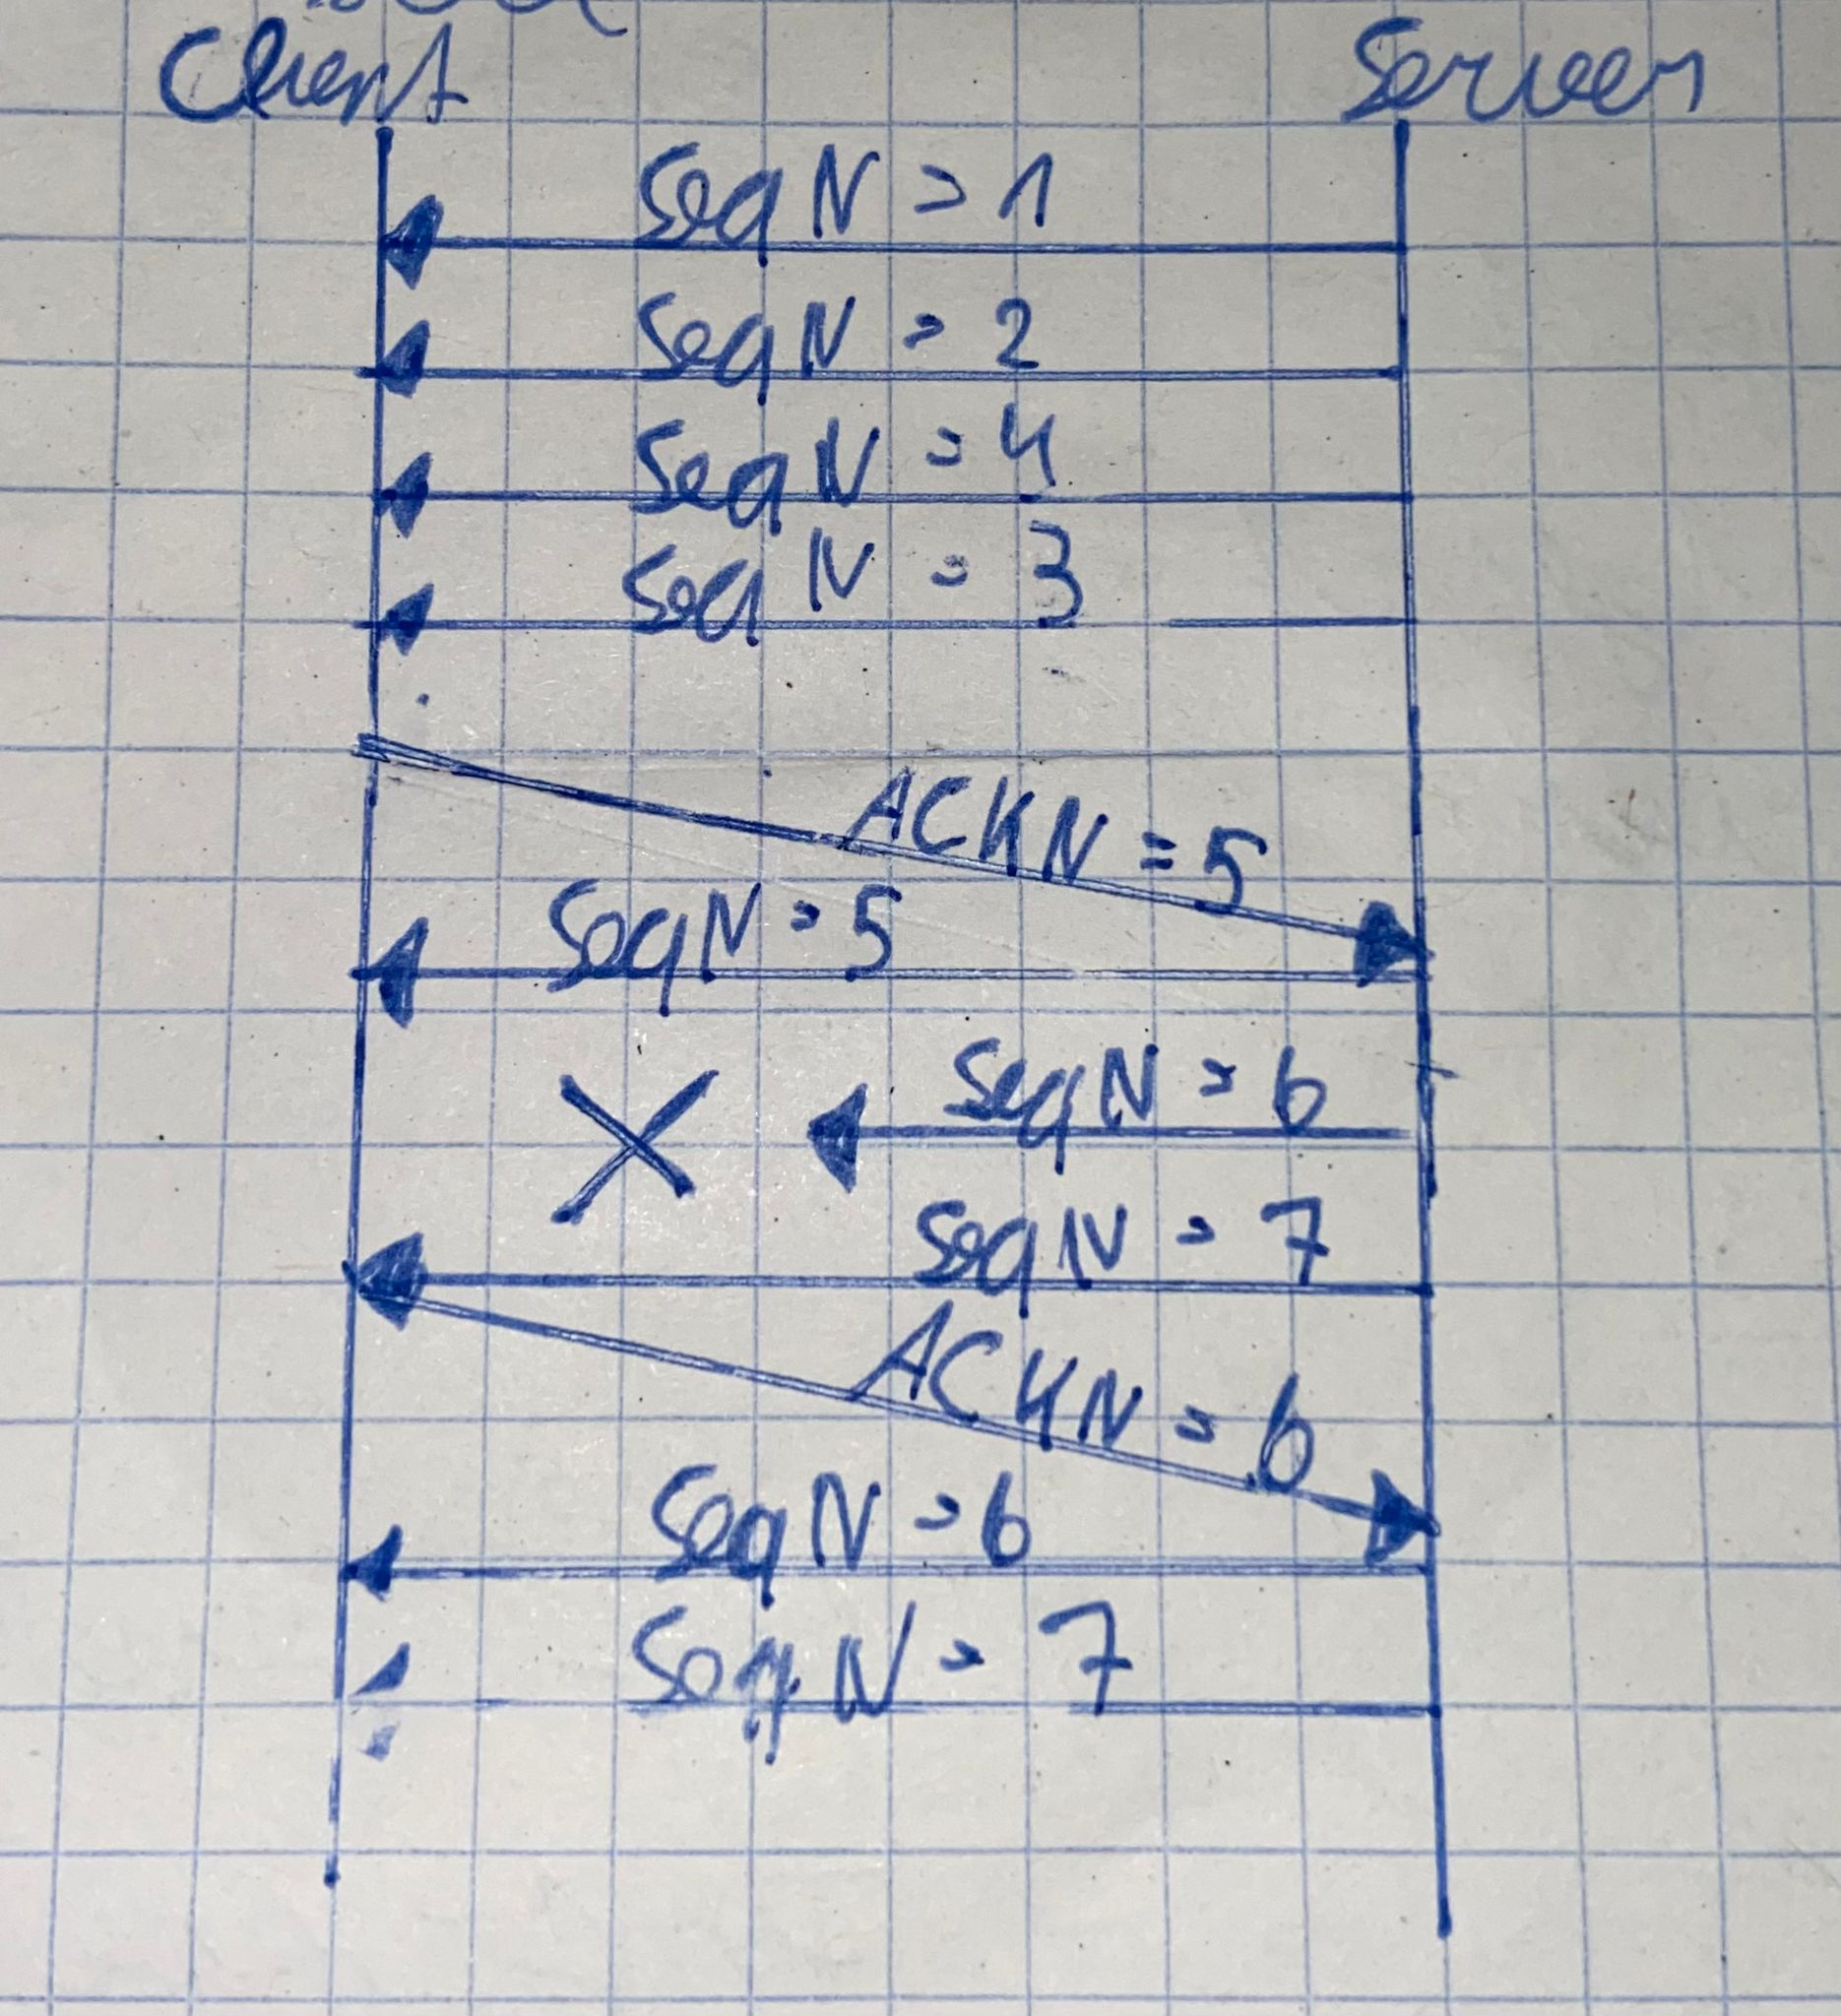
\includegraphics[width=0.8\linewidth]{figures/l4_segment.jpeg}
	\caption{Layer 4 Segmentierung}
\end{figure}

\textbf{Flow-Control} \\
Die Window Size gibt an wann das nächste ACK-Segment erwartet wird.

	\subsection{Layer 5, 6, 7 (Session, Presentation, Application)}
\subsection*{Aufgaben}
\begin{itemize}
	\item Session erstellen und halten
	\item Regelung der Session, Restart, Exchange, Idle
	\item Format und Präsentation der Daten
	\item Verschlüsselung und Komprimierung der Daten
	\item Anwendungsspezifische Informationen
\end{itemize}
\textbf{Protokolle:} HTTP/HTTPS, FTP, Telnet/SSH, DHCP, DNS, SMTP, POP, IMAP

\subsection*{DNS (Port 53, UDP)}
Um zu einer Domain die passende IP-Adresse zu finden.
Typische DNS-Server: 8.8.8.8

\begin{figure}[H]
	\centering
	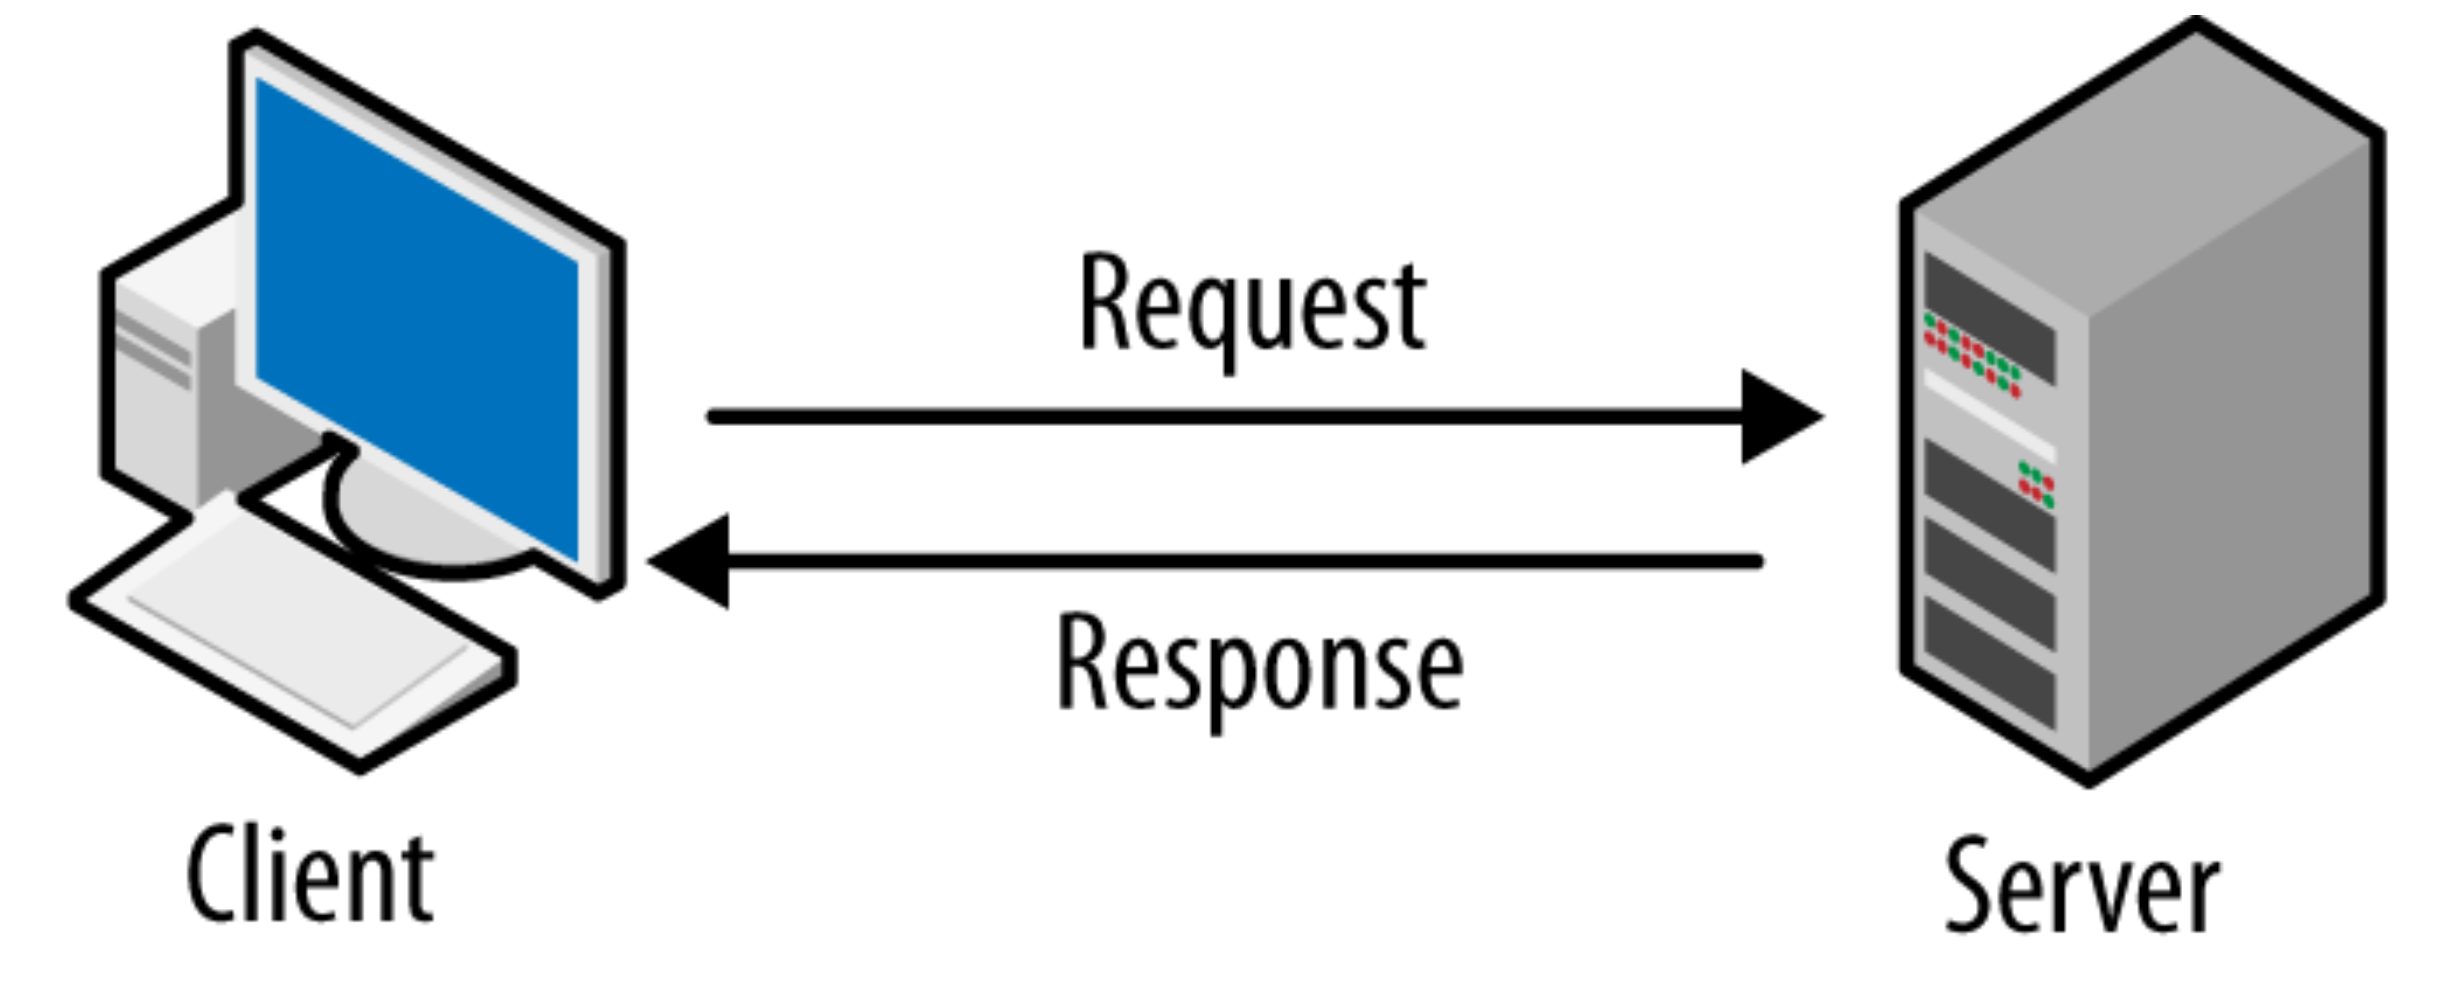
\includegraphics[width=0.8\linewidth]{figures/request_response.png}
	\caption{Request/Response Modell}
\end{figure}

\subsection*{Einträge}
A ... IPv4-Endgerät \\
AAAA ... IPv6-Endgerät \\
MX ... Mail-Server

\subsection*{Hierarchisches DNS-Modell}
\begin{figure}[H]
	\centering
	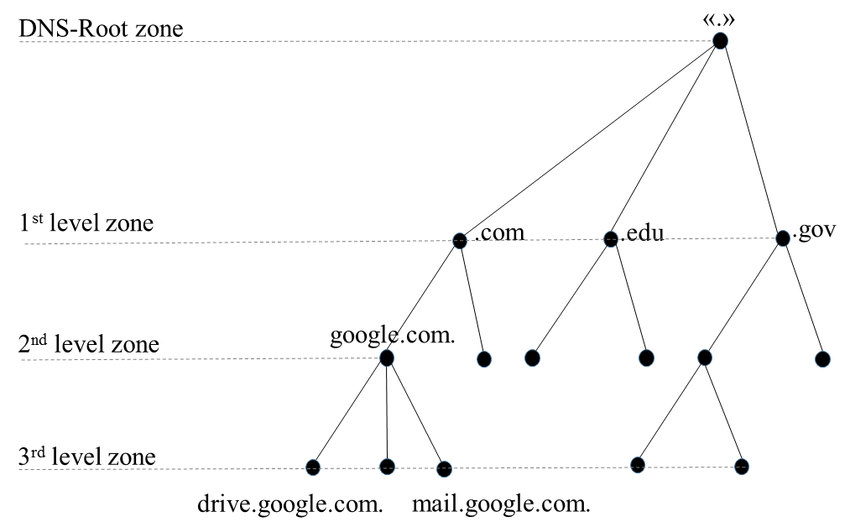
\includegraphics[width=0.8\linewidth]{figures/dns_hierarchy.png}
	\caption{DNS-Hierarchie}
\end{figure}
Falls der DNS-Server keinen Eintrag findet, wird das Paket weitergeleitet. Der Client speichert die erhaltenen DNS-Einträge.

\subsection*{DHCP (Port 67/68, UDP)}
Die Hosts erhalten dynamisch eine IP-Konfiguration (IP-Adresse, Subnetzmaske, Default Gateway, DNS-Server, Lease Time,...).

\begin{figure}[H]
	\centering
	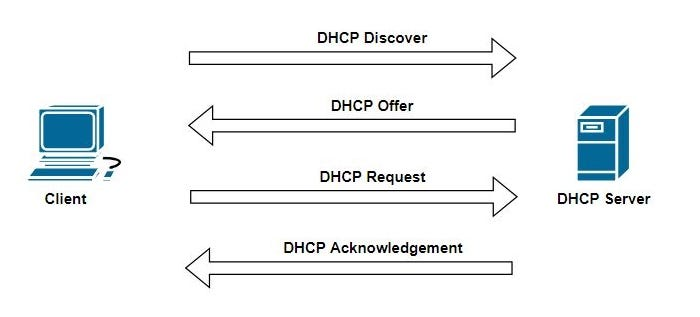
\includegraphics[width=0.8\linewidth]{figures/dhcp_handshake.jpg}
	\caption{DHCP-Handshake}
\end{figure}
DHCP-Discover ... Broadcast \\
DHCP-Offer ... Unicast \\
DHCP-Request ... Broadcast \\
DHCP-ACK ... Unicast \\ 
\textbf{Achtung:} DHCP-Spoofing

\subsection*{HTTP/HTTPS (Port 80/443, TCP)}
\begin{figure}[H]
	\centering
	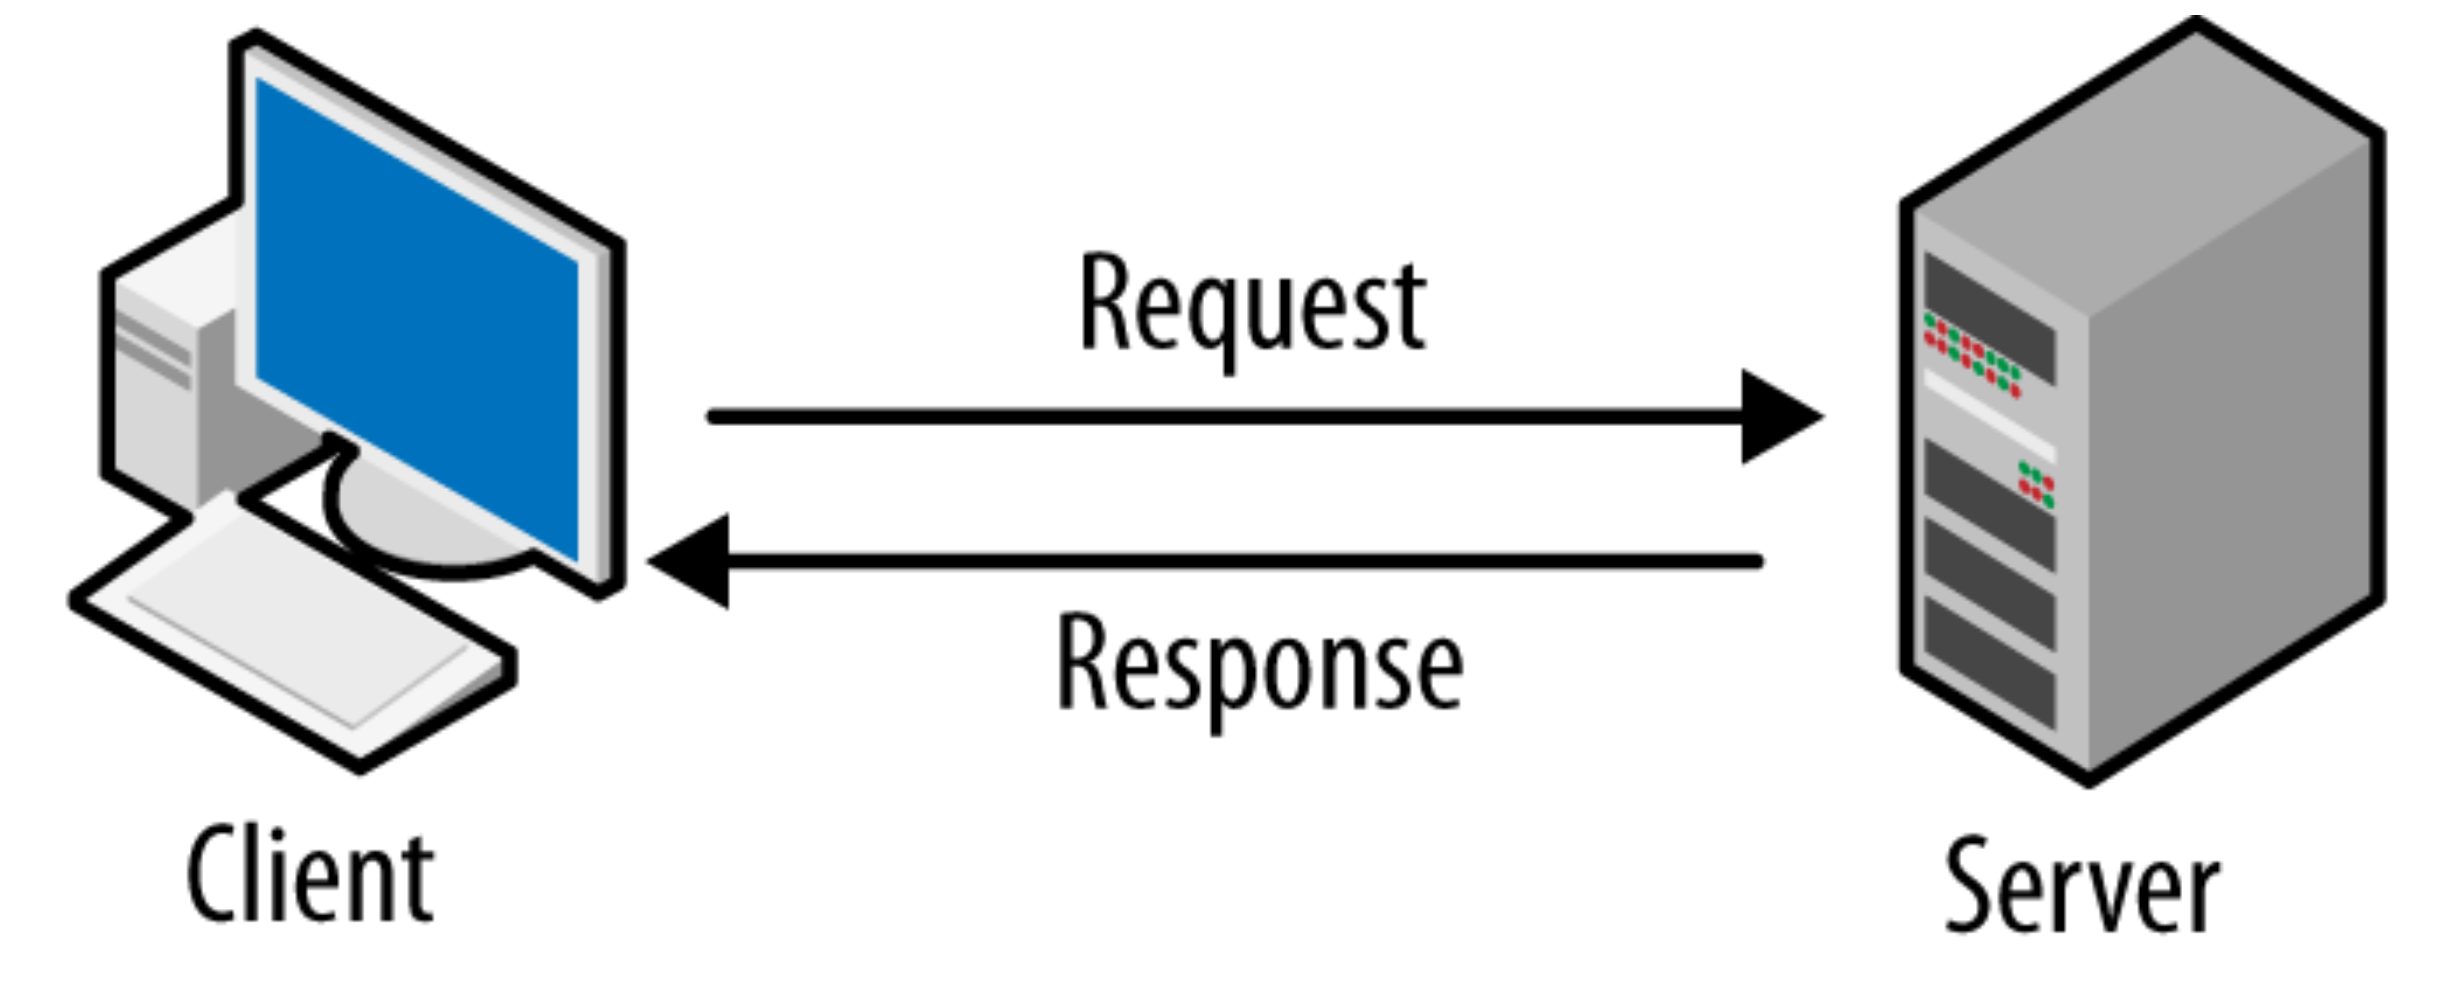
\includegraphics[width=0.8\linewidth]{figures/request_response.png}
	\caption{Request/Response Modell}
\end{figure}

\begin{table}[H]
	\begin{tabular}{c|c|c|c}
		URL: & https:// & www.google.com/ & index.html \\
		\hline
		& Protokoll & Domain IP-Adresse (DNS) & Ordnerstruktur, Datei
	\end{tabular}
\end{table}

\subsection*{Befehle}
Get, Post, Put, Delete,...

Bei HTTP ist alles im Klartext. \\
Bei HTTPS wird zusätzlich mit SSL/TLS verschlüsselt.

\subsection*{E-Mail}
\begin{table}[H]
	\begin{tabular}{c|c|c|c}
		E-Mail-Adresse: & name & @ & gmail.com \\
		\hline
		& Benutzername & & Domain
	\end{tabular}
\end{table}

\subsection*{SMTP (Port 25, TCP)}
Senden von Emails. Wird zum Senden von Mails und dem Weiterleiten zum Zielserver benutzt. SMTP kann zusätzlich Feedback geben (z.b. Ziel nicht erreichbar,...).

\subsection*{POP (Port 110, TCP)}
Empfangen von E-Mails. Man erhält vom Server das Original. Die Mail wird am Server gelöscht (Vorteil: Speicherplatz, Security).

\subsection*{IMAP (Port 143, TCP)}
Empfangen von E-Mails. Man erhält vom Server eine Kopie. Das Original bleibt am Server gespeichert (Vorteil: Verbindung mit mehreren Geräten ist praktisch, Backup).

	
	\section{VLANs}
Ein physisches Netz wird in mehrere logische Teilnetze (Layer 2) unterteilt.
\begin{table}[H]
	\begin{tabular}{l|l}
		\multicolumn{1}{c|}{Vorteile} & \multicolumn{1}{c}{Nachteile} \\
		\hline
		Kosten & (Konfiguration) \\
		Security &  \\
		Flusskontrolle &  \\
		Übersicht &  \\
		kleinere Broadcast-Domain &  \\
		Effizienz \& Performance & 
	\end{tabular}
\end{table}

\subsection*{Arten von VLANs}
\begin{itemize}
	\item Daten VLANs
	\item Default VLAN (bei cisco 1)
	\item Voice VLAN
	\item Management VLAN
	\item Native VLAN (Frames ohne VLAN-Tag kommen in das Native VLAN, kann nur am Trnk passieren)
\end{itemize}

Access Ports transportieren nur ein VLAN. \\
Trunk Ports können viele VLANs transportieren. \\
Die VLAN-Namen werden zusätzlich im Header eingetragen (802.1q $\rightarrow$ Ethernet)

\subsection*{ACL}
Je nach IP-Adresse (Standard) bzw. Port (Extended) wird ein Packet blockiert oder zugelassen.

\subsection*{Wildcardmask}
Subnetzmaske: Teilt IP-Adresse in Netz- und Hostteil \\
1 ... Netzteil (relevant für das Netz) \\
0 ... Hostteil (irrelevant für das Netz) \\
$\rightarrow$ unflexibel

Wildcardmaske '1' \& '0' können beliebig gezählt werden \\
0 ... relevantes Bit der IP-Adresse \\
1 ... nicht relevantes Bit der IP-Adresse

\begin{tabbing}
	255.255.255.255 ~~~ \= any \\
	0.0.0.0 ~~~~~~~~~~~~~~~ \= host
\end{tabbing}

\subsection*{Position der Wildcardmask}
\begin{figure}[H]
	\centering
	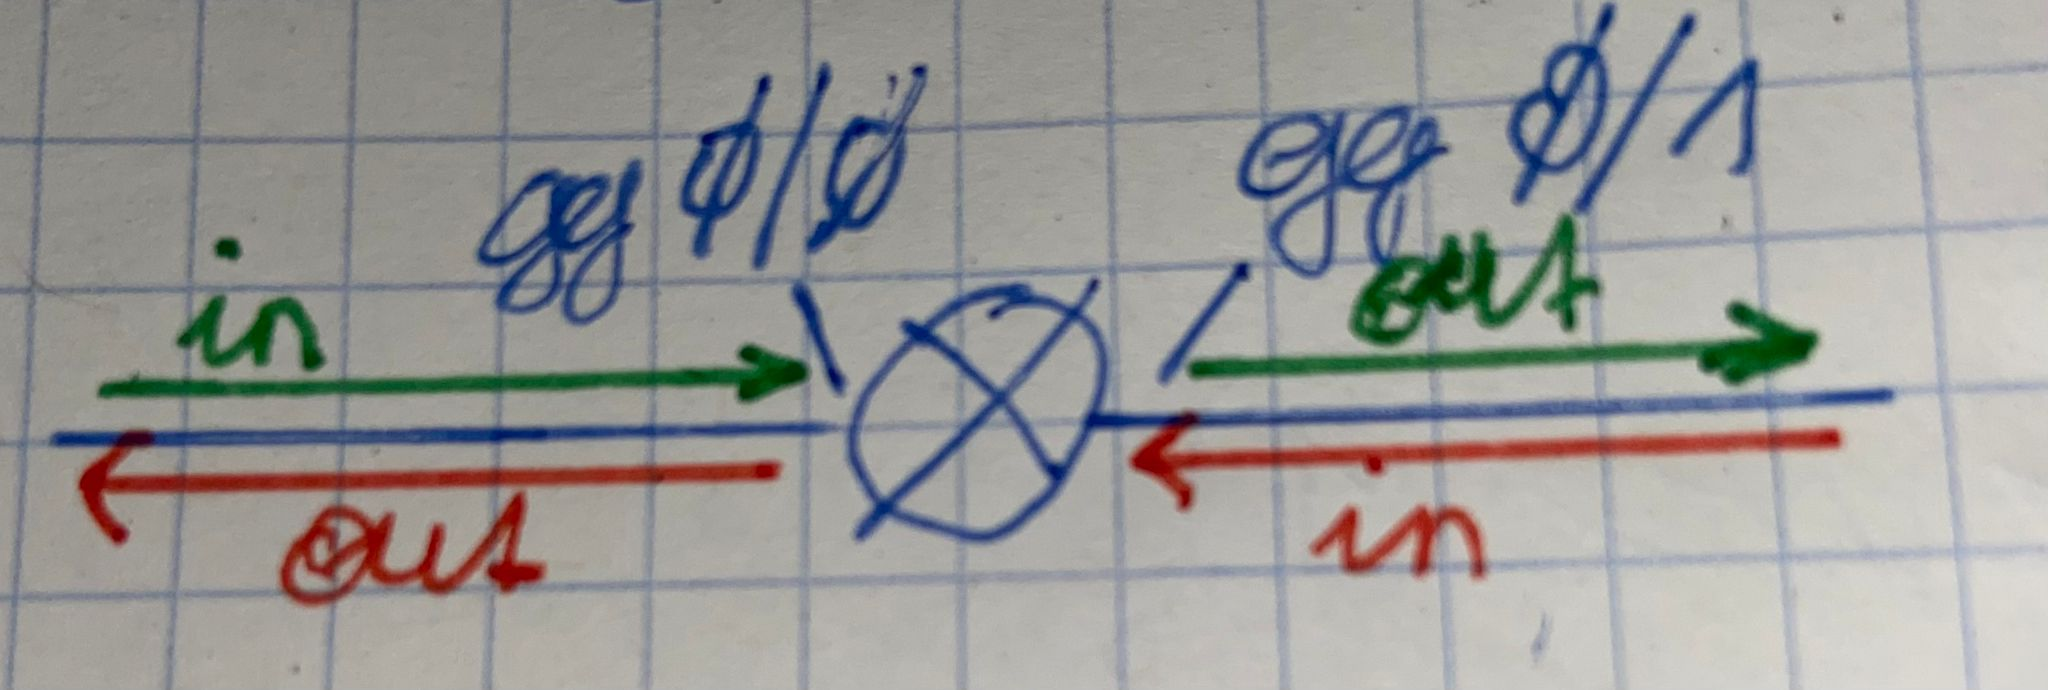
\includegraphics[width=0.8\linewidth]{figures/wildcard.jpeg}
	\caption{Position der Wildcardmask}
\end{figure}

Regeln bei Interfaces: eingehend \& ausgehend \\
\textbf{Achtung} Die letzte Zeile in jeder ACL ist 'deny any'.

\subsection*{Static NAT (1:1 Mapping)}
\begin{figure}[H]
	\centering
	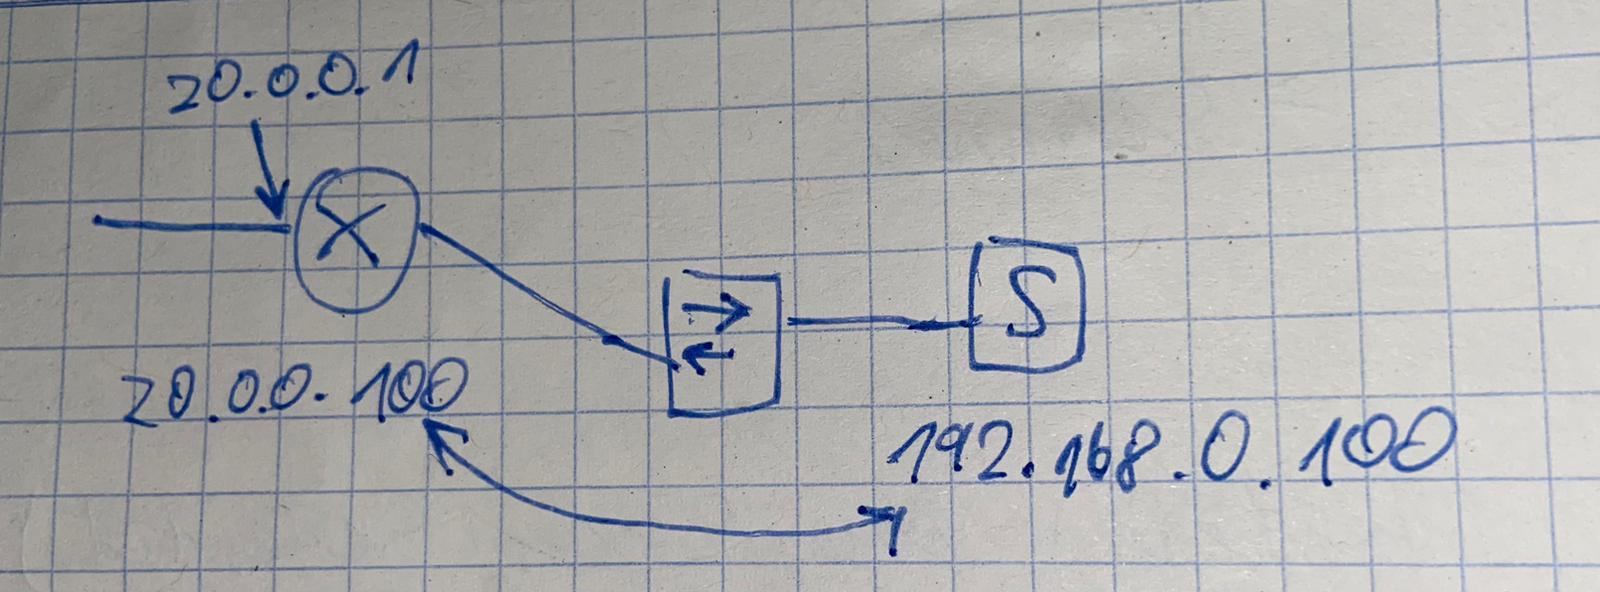
\includegraphics[width=0.8\linewidth]{figures/static_nat.jpeg}
	\caption{Static NAT, 1:1 Mapping}
\end{figure}

\subsection*{NAT mit PAT (n:1 Mapping)}
\begin{figure}[H]
	\centering
	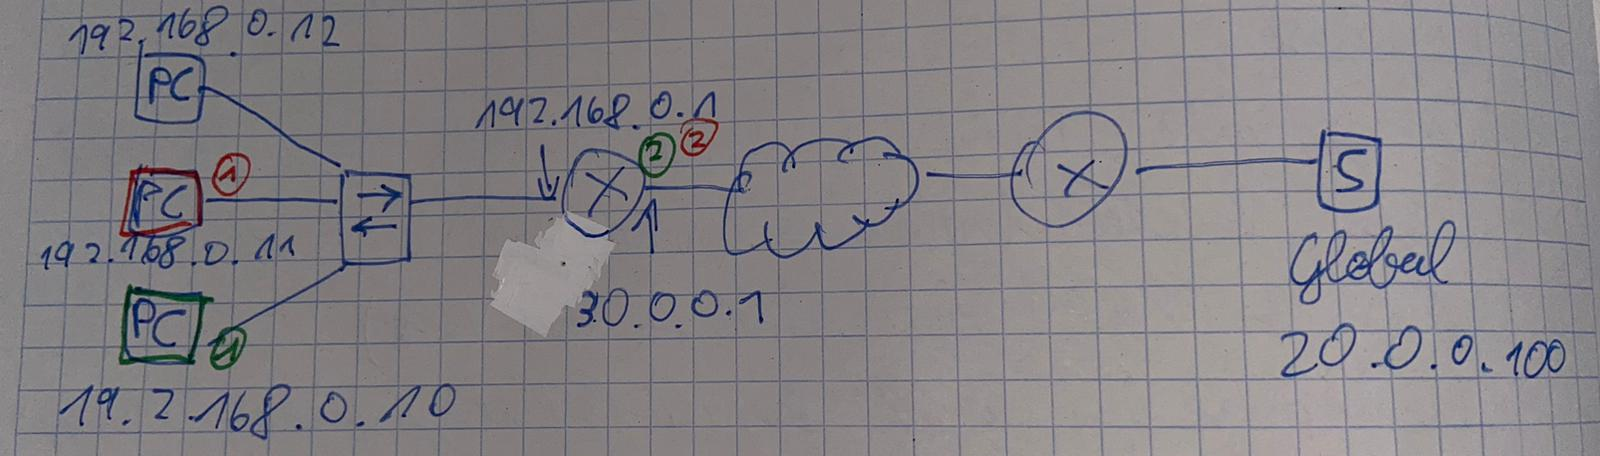
\includegraphics[width=0.8\linewidth]{figures/pat_nat.jpeg}
	\caption{NAT mit PAT, n:1 Mapping}
\end{figure}

\begin{table}[H]
	\begin{tabular}{c|cccc}
		& Source IP & Destination IP & Source Port & Destination Port \\
		\hline
		{\color[HTML]{32CB00} 1} & 192.168.0.10 & 20.0.0.100 & 51000 & 443 \\
		{\color[HTML]{FE0000} 1} & 192.168.0.11 & 20.0.0.100 & 51000 & 443 \\
		{\color[HTML]{32CB00} 2} & 30.0.0.1 & 20.0.0.100 & 51000 & 443 \\
		{\color[HTML]{FE0000} 2} & 30.0.0.1 & 20.0.0.100 & 51001 & 443
	\end{tabular}
\end{table}

\begin{table}[H]
	\begin{tabular}{p{\dimexpr 0.5\linewidth-2\tabcolsep} | p{\dimexpr 0.5\linewidth-2\tabcolsep}}
		\multicolumn{1}{c}{\textbf{Vorteile}} & \multicolumn{1}{|c}{\textbf{Nachteile}} \\
		\hline
		\textbf{+ IP-Adressen sparen} & \textbf{- Ende zw. Ende Verbindung geht verloren} \\
		+ Security & - Paketverfolgung und Troubleshooting \\
		+ IP-Adressen Schema kann frei gewählt werden & - Performance \\
	\end{tabular}
\end{table}


		
	\part{5BHWII}	
	\chapter{Routing}
Router muss entscheiden welcher Weg der 'beste' Weg ist. \\
$\rightarrow$ bei welchen Interface (Netz) rausschicken = Routing

Routing Tabelle wird durch ...
\begin{itemize}
	\item dynamisch (Routingprotkolle)
	\item statische Einträge
\end{itemize}
... aufgebaut (in der Praxis meist aus Mischung).

Router wählt Route mit am meisten Bits bei Ziel übereinstimmung (Vergleich von Route \& Destination IP).

\section*{1) Einträge in Routing Tabelle}
\begin{itemize}
	\item Direkt verbundene Netze: Aktive \& angeschlossene Netze am Router mit IP-Konfiguration $\rightarrow$ automatisch (Status Code: C, L)
	\item Remote Netze: statisch oder dynamisch (vom Routingprotokoll abhängig) eingetragen (Status Code: S, R, O, E,...)
	\item Default Route (gateway of last resort): Next Hop falls der Router keine passende Route findet, statisch oder dynamisch. \\ Route: 0.0.0.0 / 0 ... 0 Bits müssen übereinstimmen
\end{itemize}

\section*{2) Eintrag in Cisco CLI}
\begin{table}[H]
	\begin{tabular}{cccccc}
		R & 30.0.4.0/24 & [120/7] & via 10.0.3.2 & 00:13:29 & Serial 10/1/1 \\
		Status & Ziel & AD/Metrik & IP (ausgehendes Interface) & Zeitstempel & Interface
	\end{tabular}
\end{table}

\subsection*{Status Code}
\begin{tabbing}
	C ... connected ~~~ \= Direkt verbundene Netzte \\
	L ... local ~~~ \= IP vom Interface, lokale Route \\
	S ... static ~~~ \= statisch eingegebene Route \\
	R ... RIP ~~~ \= entsprechendes Routingprotokoll \\
	O ... OSPF ~~~ \= entsprechendes Routingprotokoll \\
	E ... EIGRP ~~~ \= entsprechendes Routingprotokoll
\end{tabbing}

\subsection*{Ziel}
IP-Adresse des Zielnetzes mit Präfix (nicht unbedingt Subnetzmaske). Es müssen die angegebene Anzahl von Bits (Präfix) mit Destination IP-Adresse übereinstimmen (damit Route in Frage kommt). Route mit am meisten übereinstimmenden Bits (von links). \\
Problem: es wird keine Subnetzmaske der Destination IP mitgeschickt $\rightarrow$ normalerweise auch nicht bekannt.

\begin{center}
\begin{tabular}{ll}
	\multicolumn{2}{l}{Dest IP: 172.16.0.10 (letztes Oktett: 00001010)} \\
	\hline
	1) 172.16.0.0 /16 & Bis Bit 16 übereinstimmend \\
	2) 172.16.0.0 /24 & Bis Bit 24 übereinstimmend \\
	3) 172.16.0.0 /26 & Bis Bit 26 übereinstimmend \\
	4) 172.16.0.0 /30 & Bis Bit 29 nicht übereinstimmend \\
	5) 172.17.0.0 /24 & am 2. Oktett stimmt es nicht überein
\end{tabular}
\end{center}

Router wählt 3. Variante (???). Dort stimmt die angegebene Anzahl an Bits (Präfix) überein

\subsection*{AD: Administrative Distanz}
Router kann Route über mehrere Arten lernen (z.B. statisch, RIP, OSPF,...). AD gibt an wie 'vertrauenswürdig' eine Route ist. Router verwendet Route mit niedrigster AD, andere Routen sind Backups und werden vorerst nicht im Routing Table angezeigt.\\
$\rightarrow$ wenn 'beste' Route ausfällt wird nächst beste verwendet

Standard Werte bei Cisco Routern
\begin{table}[H]
	\begin{tabular}{rc}
		& AD \\
		\hline
		Direkte Routen & 0 \\
		Statische Routen & 1 \\
		EIGRP & 90 \\
		OSPF & 110 \\
		RIP & 120 \\
	\end{tabular}
\end{table}

\subsection*{Metrik}
Von einem Routingprotokoll kann der Router mehrere Routen zum gleichen Ziel lernen. Die Metrik gibt an, 'wie weit' das Ziel entfernt ist. Der Router verwendet die Route mit der geringsten Metrik. Falls eine Route ausfällt, wird auf Backup-Routen zurückgegriffen.

\section*{3) Statische Routen}
Werden in kleineren Netzen mit geringen Veränderungen, bei speziellen Zielnetzen oder Router mit nur einen Nachbar (Stub-Network) verwendet. \\
Problem: Statische Routen werden nicht automatisch aktualisiert und müssen händisch aktualisiert werden.

\section*{4) Dynamische Routingprotokolle}
Je nach Ablauf des Routingprotokolls unterscheidet man unterschiedliche Kategorien.
\begin{itemize}
	\item \textbf{Pfadvektorprotokolle} \\
	Diese Protokolle speichern den Pfad/Weg zum Ziel. Sie sind besonders effizient gegen Routing-Schleifen und eignen sich dadurch zum Routen von autonomen Systemen. \\
	Beispiel: BGP (Border Gateway Protocol), Metrik: Anzahl der autonomen Systemen bis zum Ziel (Zusatzinformation IGP-Metrik: wie lange dauert es durch ein autonomes System)
	\item \textbf{Distanzvektorprotokolle} \\
	Diese Protokolle speichern nur die Distanz zum Ziel \\
	Beispiel: RIP (Routing Information Protocol), Metrik: Anzahl der Hops \\
	EIGRP (Enhanced Interior Gateway Routing Protocol), Metrik: Bandbreits, Auslastung, Delay, Zuverlässigkeit \\
	EIGRP kennt die ganze Topologie im System, speichert diese aber nicht direkt ab.
	\item \textbf{Link-State-Protokolle} \\
	Diese Protokolle kennen die ganze Topologie im System. Daraus berechnet sich jeder Router die besten Routen zu allen Zielen. \\
	Beispiel: OSPF (Open Shortes Path First), Metrik: Bandbreite
\end{itemize}

\section*{5) Algorithmen zur Bestimmung des kürzesten Weges}
\begin{itemize}
	\item Bellman Ford (RIP)
	\item Dijkstra (OSPF)
	\item DUAL (EIGRP)
\end{itemize}

\subsection*{Dijkstra Algorithmus}
Ablauf: \\
1. Startknoten mit 0 markieren, alle anderen mi $\infty$: 'Distanz' und 'besucht' merken \\
2. Solange es unbesuchte Knoten gibt:
\begin{itemize}
	\item Jenen Knoten mit der kürzesten Distanz wählen
	\item Als besucht markieren
	\item Für alle unbesuchten Knoten die Distanz berechnen
	\item Falls der Wert kleiner ist, als der aktuelle, diese speichern
\end{itemize} 
	\chapter{Aufbau des Internets}
\begin{figure}[H]
	\centering
	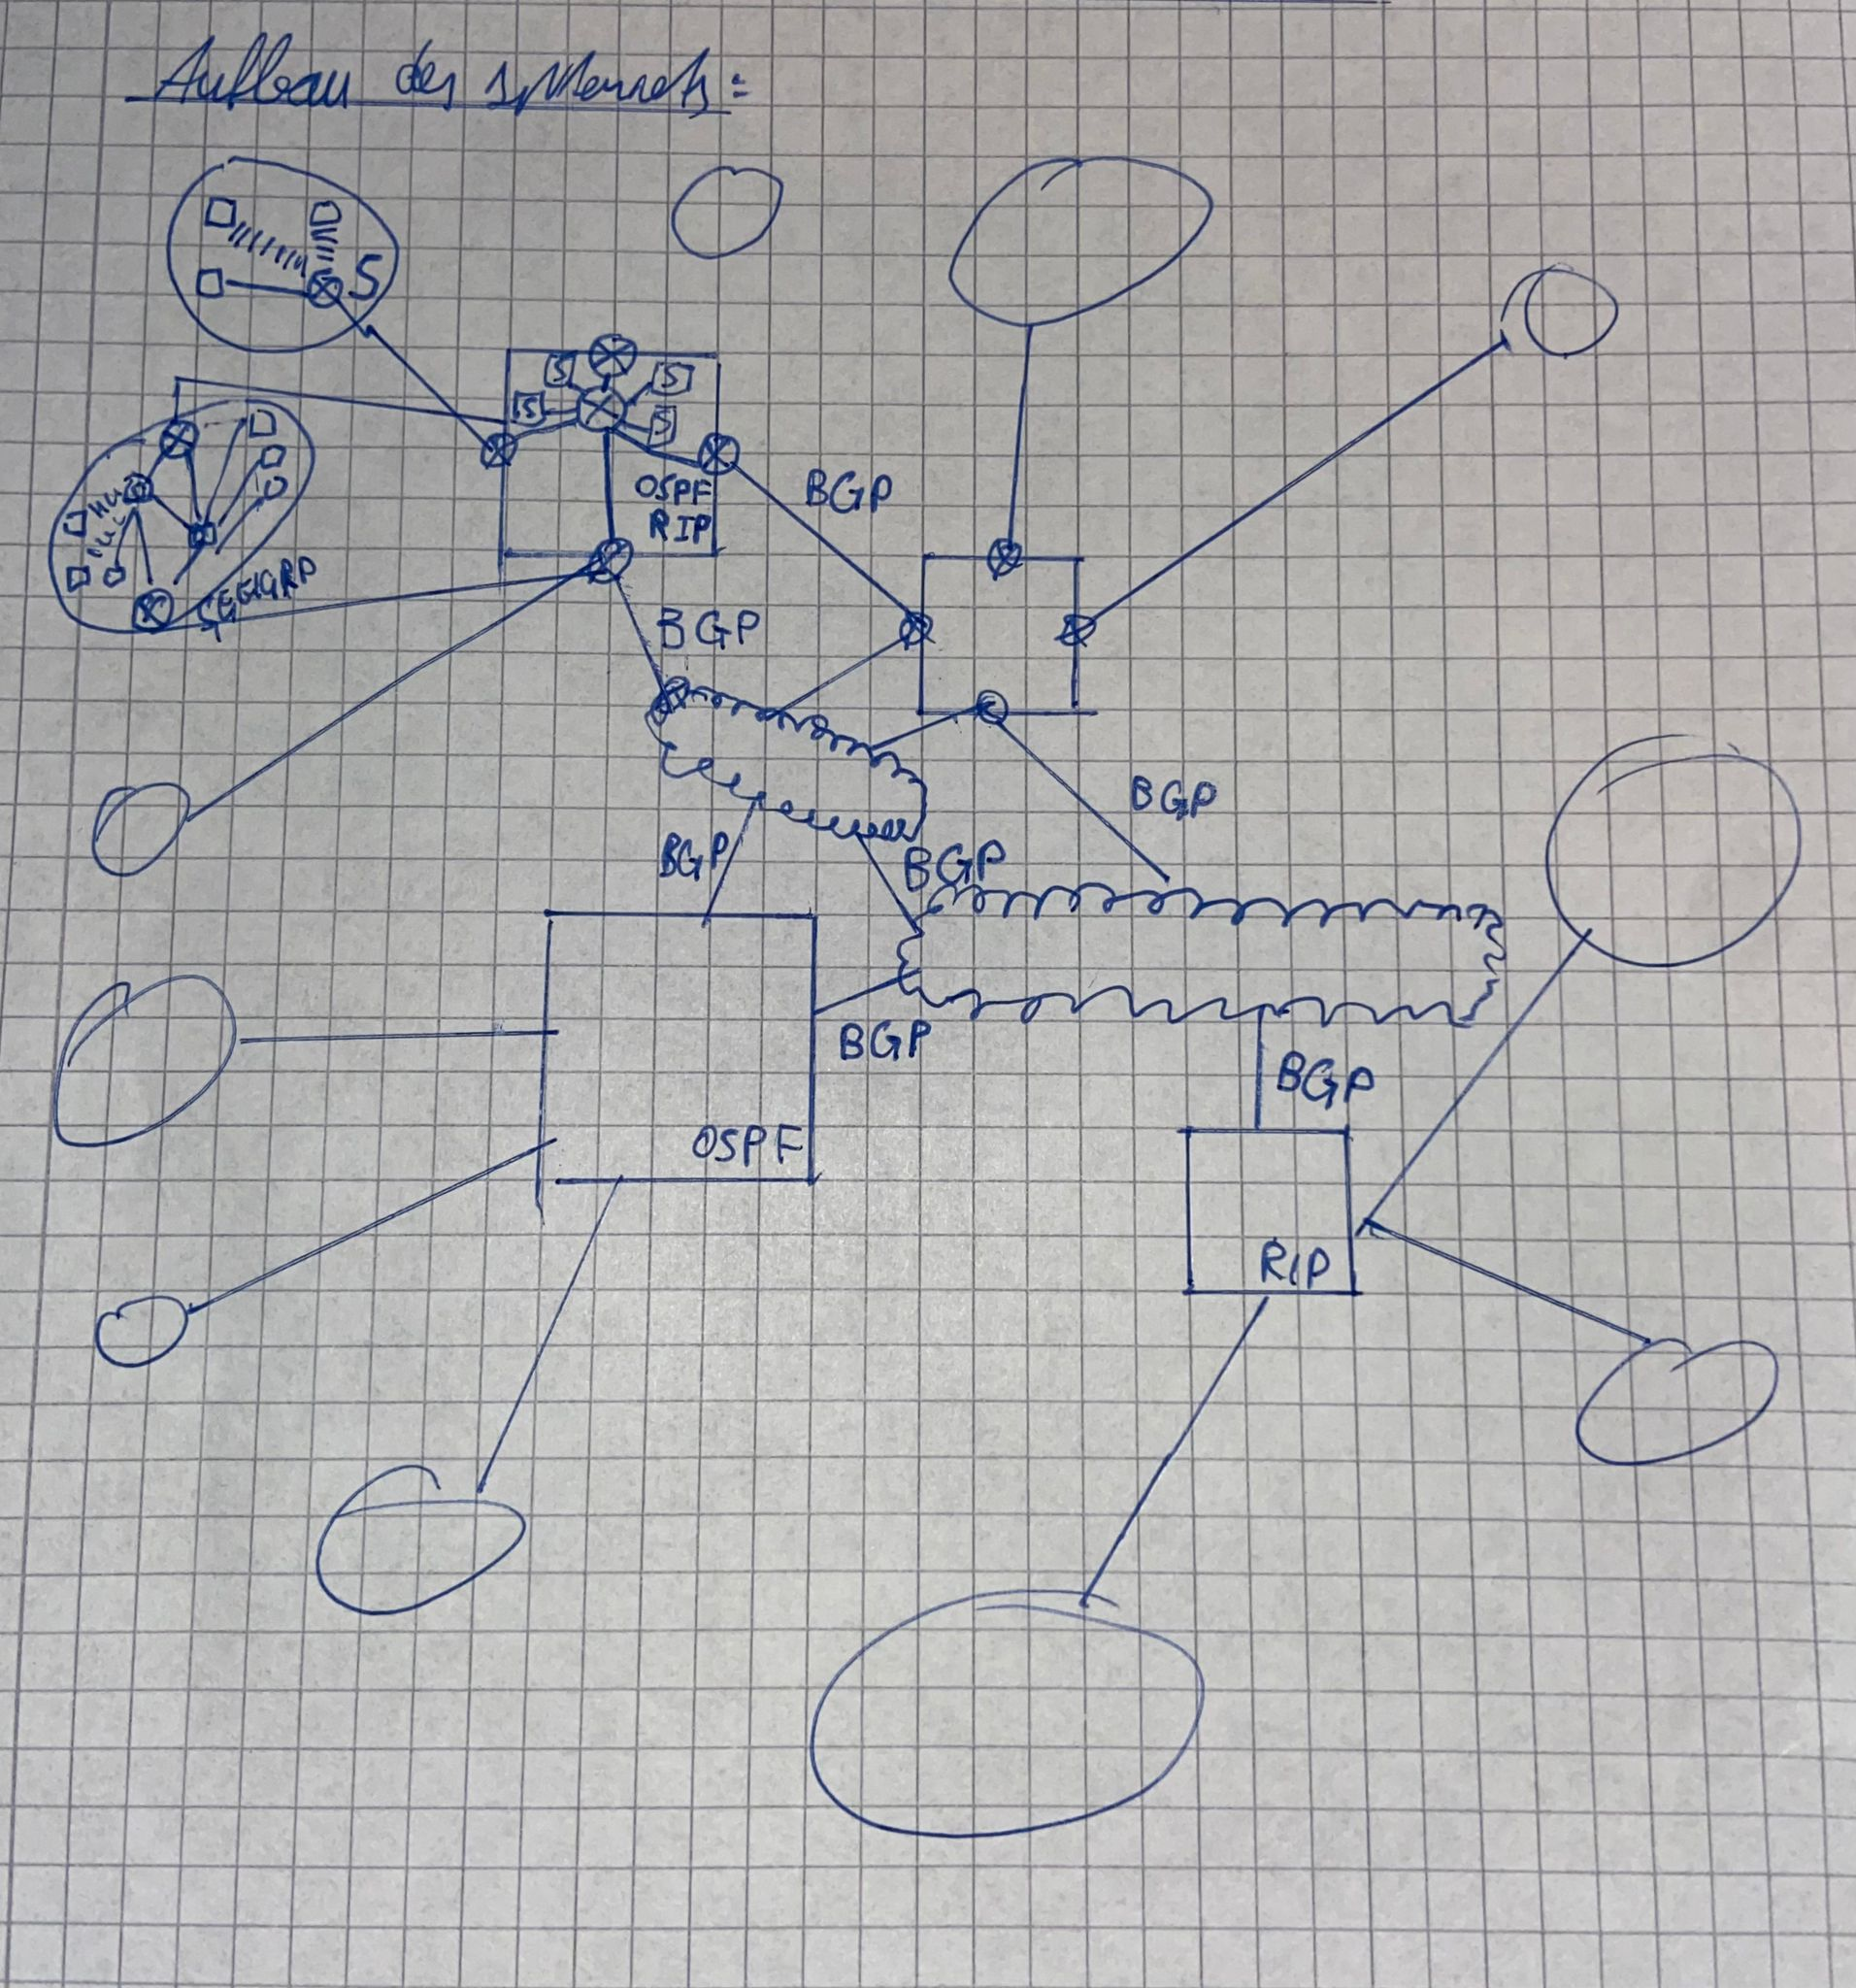
\includegraphics[width=0.8\linewidth]{figures/aufbau_internet.jpeg}
	\caption{Static NAT, 1:1 Mapping}
\end{figure}
	\chapter{IPv6}
Eine IPv6-Adresse ist eine 128 Bit Zahl. Es gibt $2^{128}$ IPv6-Adressen ($340\cdot10^{36}$).

\textbf{Schreibweise einer IPv6-Adresse} \\
\begin{itemize}
	\item Hexadezimale Schreibweise (32 Zeichen)
	\item Gruppen von 16 Bit mit : getrennt
	\item Führende Nullen werden in jeder Gruppe weggelassen
	\item Einmalig kann der längste Block an Nullen mit :: ersetzt werden
\end{itemize}

Bsp: \\
2001:ABAD:0000:0430:0000:0000:00C9:0001 \\
2001:ABAD:0:430:0:0:C9:1 \\
2001:ABAD:0:430::C9:1

\textbf{Subnetzmaske}
\begin{itemize}
	\item trennt in Netz- und Hostteil 
	\item nur noch Präfix-Notation
	\item Es wird fast nur /64 verwendet
\end{itemize}

\textbf{Idee von IPv6}
\begin{itemize}
	\item mehr IP-Adressen
	\item Problem: alle Protokolle die IPv4 verwenden müssen erneuert werden
	\item Alte Fehler/Security-Probleme beheben
	\item leichterer Header
\end{itemize}

\textbf{Übergang von IPv4 zu IPv6}
\begin{itemize}
	\item Dualer Stack
	\item Translation
	\begin{figure}[H]
		\centering
		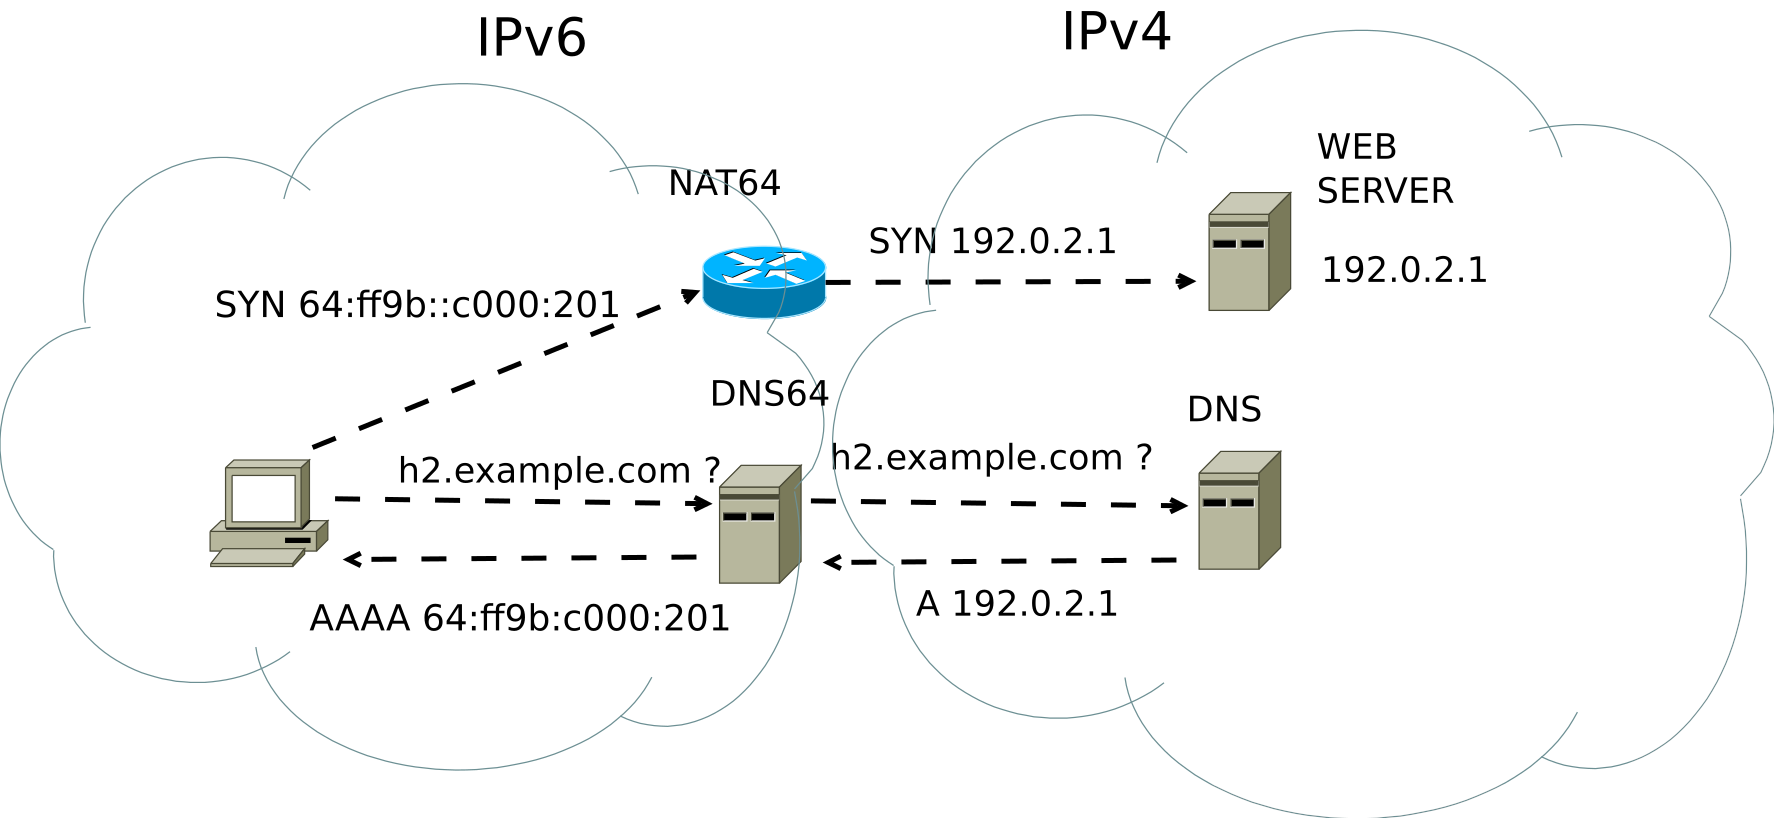
\includegraphics[width=0.7\linewidth]{figures/nat64.png}
		\caption{IPv4-IPv6 Translation mit NAT64}
	\end{figure}
	\item Tunneling
		\begin{figure}[H]
		\centering
		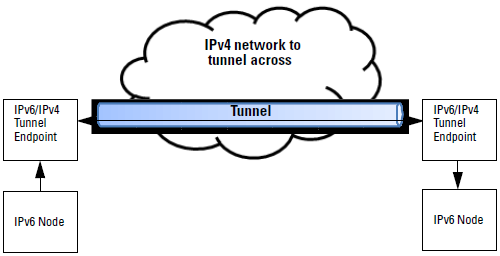
\includegraphics[width=0.7\linewidth]{figures/ipv6_tunneling.png}
		\caption{IPv4-IPv6 Tunneling}
	\end{figure}
\end{itemize}

\textbf{Kommunikationsarten}
\begin{itemize}
	\item Unicast
	\item Multicast \\
	ff02::1 ... all-nodes-multicast (Broadcast) \\
	ff02::2 ... all-router-multicast
	\item Anycast (der 'nägeste' einer Gruppe bekommt den Anycast)
\end{itemize}

\textbf{IPv6-Unicast Adressen} \\
\begin{itemize}
	\item Global Unicast Adressen 2000-3fff (vgl. öffentliche IP)
	\item Link Local Adressen fe80-febf (für das lokale Netz, nicht routbar)
	\item loopback ::1 (vgl. IPv4 127.0.0.1)
	\item Unspecified Adress :: (vgl. IPv4 0.0.0.0)
	\item Unique Local fc00-fdff (vgl. IPv4 NAT)
	\item Embedded IPv4
\end{itemize}

\textbf{IP-Konfiguration}
\begin{itemize}
	\item statisch (GUA, LLA)
	\item dynamisch
	\begin{itemize}
		\item SLAAC
		\item SLAAC mit stateless DHCPv6 Server
		\item DHCPv6
	\end{itemize}
\end{itemize}

\textbf{SLAAC} \\
\begin{figure}[H]
	\centering
	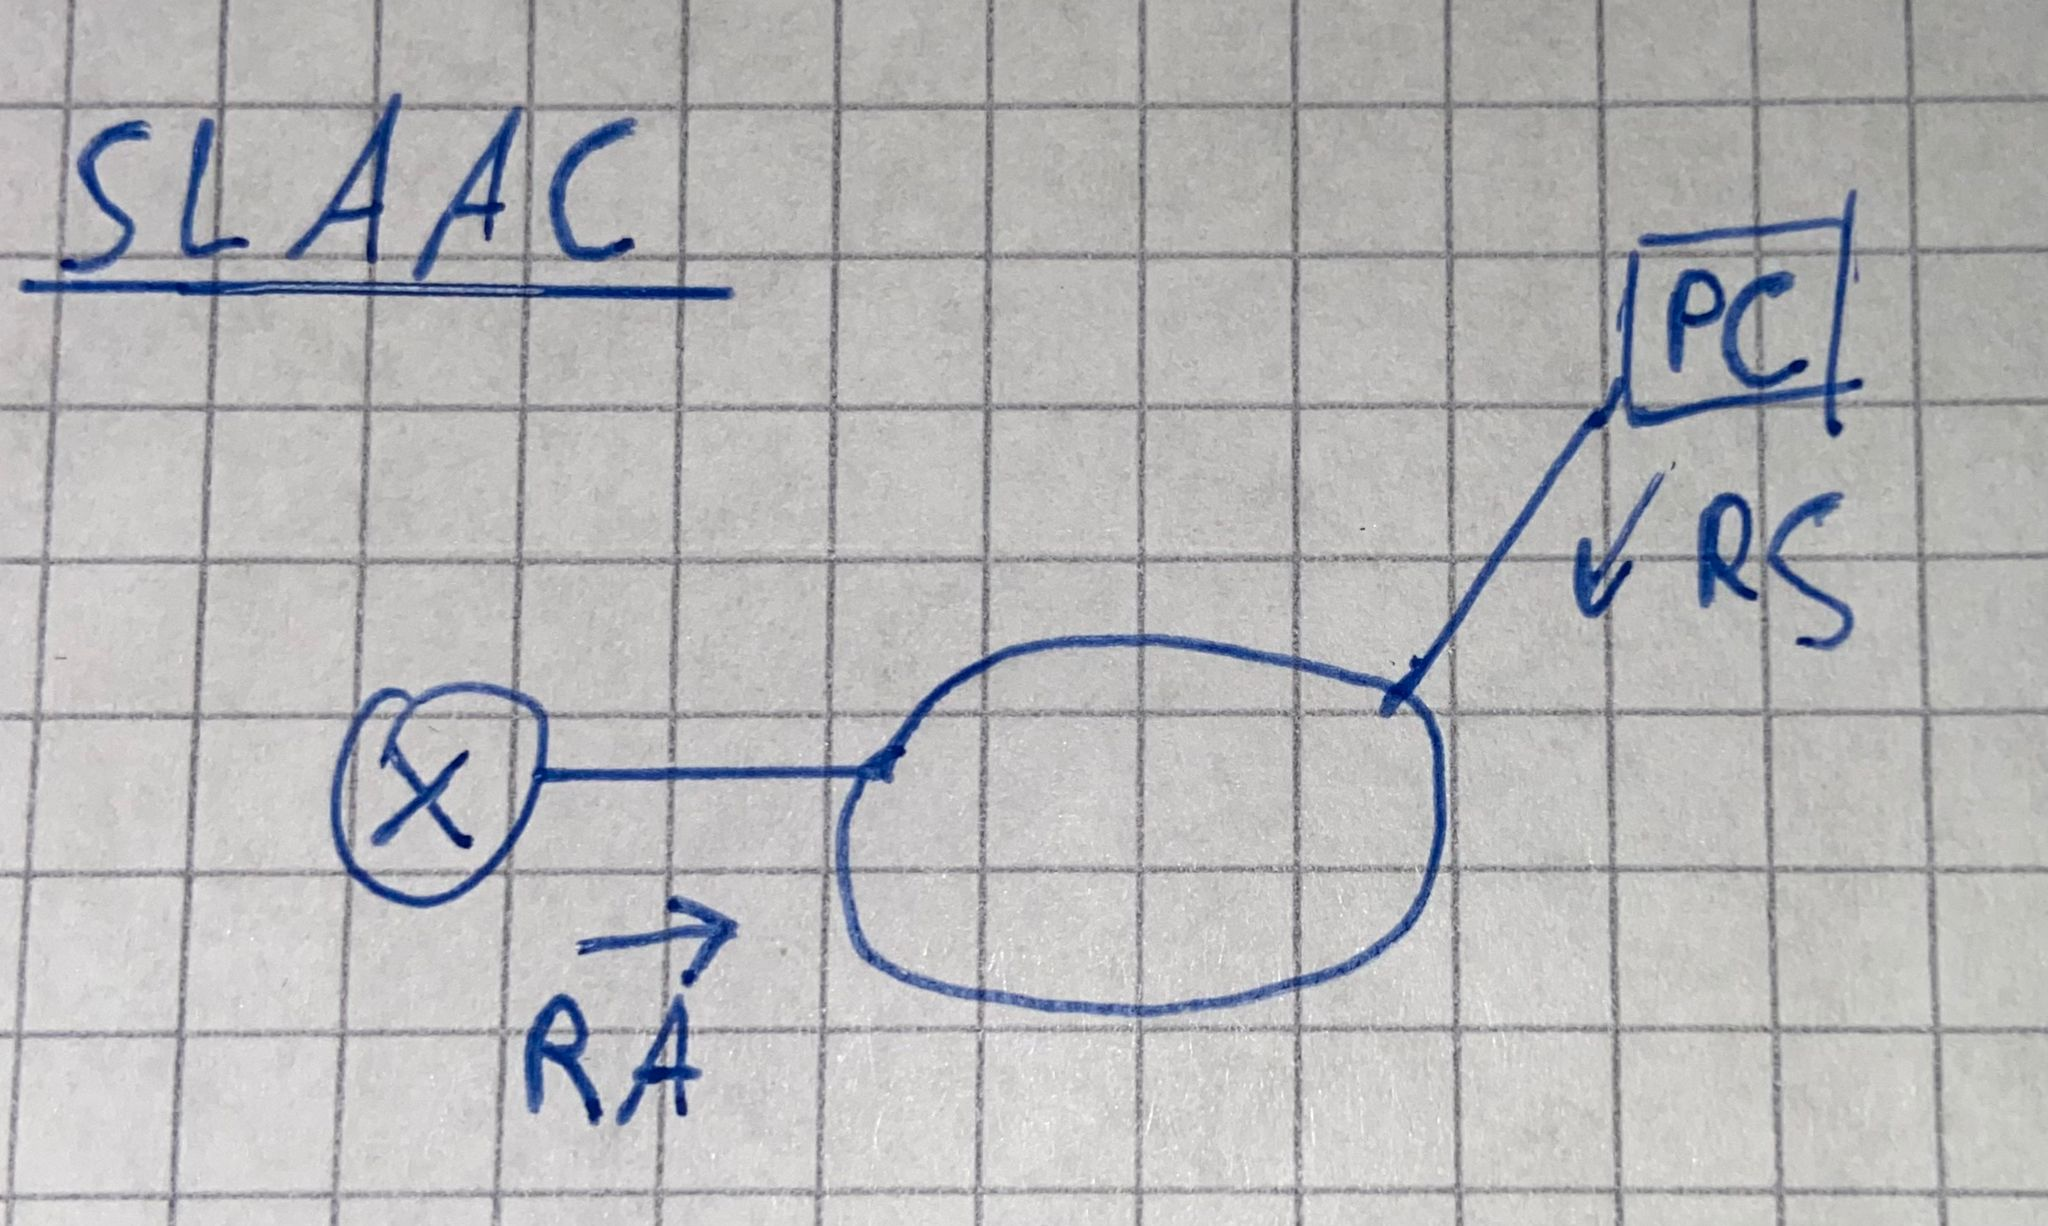
\includegraphics[width=0.8\linewidth]{figures/slaac.jpeg}
	\caption{SLAAC}
\end{figure}
Router senden (ca. alle 200s) ein RA-Paket (Router Advertisement) aus. Dies enthält die wichtigsten Informationen für die Hosts (Präfix, Präfix-Länge, Default-Gateway). Die Hosts geben sich dann selbst die IPv6-Adresse. \\
Hostteil
\begin{itemize}
	\item Zufallszahl (ND-Protokoll)
	\item EUI-64 (MAC-Adresse)
\end{itemize}
Die Hosts können RS (Router Solicitation) Pakete aussenden um das RA-Paket anzufordern.




	\chapter{WLAN (Wireless Local Area Network)}
Bei einem drahtlosen Netzwerk findet die Übertragung ohne Kabel statt. Es werden elektromagnetische Wellen über die Luft übertragen. Für die drahtlose Übertragung im Netzwerk bedeutet dies, dass sich Layer 1 und Layer 2 ändern. Die darüber liegenden Layer bleiben unverändert. Durch diese Änderung der Übertragungsart ergeben sich einige Vorteile aber auch Nachteile.

\begin{center}
	\begin{tabular}{p{\dimexpr 0.5\linewidth-2\tabcolsep} | p{\dimexpr 0.5\linewidth-2\tabcolsep}}
		\multicolumn{1}{c|}{\textbf{Vorteile}} & \multicolumn{1}{c}{\textbf{Nachteile}} \\
		\hline
		+ BYOD: bring your own device & - Geteiltes Medium für viele Teilnehmen \\
		+ Kosten: Besonders in bestehenden Gebäuden & - Störungen \\
		+ Anpassungsfähigkeit & - Geschwindigkeit und Reichweite \\
		& - Security \\
	\end{tabular}
\end{center}

\subsection*{Antennen}
Antennen sind die Grundlage für eine Übertragung über die Luft. Sie geben ein Signal in die Luft ab (Senderantenne) und können es auch wieder aus der Luft aufgreifen (Empfängerantenne). Je nach Anwendung eignen sich verschiedene Arten von Antennen.
\begin{itemize}
	\item Omnidirektionale Antennen: senden in alle Richtungen (Kugel)
	\item Direkte Antennen: Können gezielt senden
	\item MIMO (multiple input multiple output) Antennen: aktuell meist 8 Antennen
\end{itemize}

\subsection*{Arten von Wireless Netzwerken}
Wie auch schon bei den verkabelten Netzen unterscheidet man Netzte nach ihrer Größe. Je nach Größe ergeben sich unterschiedliche Anforderungen und Schwierigkeiten.
\begin{itemize}
	\item \textbf{WPAN:} kurze Distanz (ca 10m), Frequenz meist 2.4 GHz z.B. Bluetooth, Zigbee
	\item \textbf{WLAN:} mittlere Distanz (ca 100m), Frequenz ist 2.4 GHz oder 5 GHz z.B. Wifi
	\item \textbf{WMAN:} große Distanz (kann sehr unterschiedlich sein), Frequenz zwischen 2 und 66 GHz z.B. Wifi, WiMax
	\item \textbf{WWAN:} riesige Distanzen (bis zu 50km), Frequenz zwischen 2 und 66 GHz z.B. WiMax
\end{itemize}

\subsection*{Technologien von Wireless Netzwerken}
Es gibt unterschiedliche Technologien dir drahtlos übertragen. Je nach Reichweite und Anwendungsgebiete sind unterschiedliche Technologien sinnvoll. Nicht alle Technologien sind dazu geeignet oder dafür entworfen um Netzwerkdaten zu übertragen. Manche Technologien können dies trotzdem umsetzen.
\begin{itemize}
	\item \textbf{Wifi} (IEEE 802.11)
	\item \textbf{Bluetooth} (IEEE 802.15)
	\item \textbf{WiMax} (IEEE 802.16)
	\item \textbf{Satelliten Breitband:} kann als Internetzugang genutzt werden, z.B. Starlink (Oktober 2023 ca. 5000 Geräte, in einer Entfernung von 500 bis 600km, beantragt sind 22.000 Satelliten)
	\item \textbf{Mobilfunk Breitband:} viele verschiedene Standards die meist nach gravierenden Änderungen (Generationen) unterteilt werden. Bei der Änderung in eine neue Generation ist die Geschwindigkeit immer ein entscheidender Faktor (3G $\rightarrow$ 10x $\rightarrow$ 4G $\rightarrow$ 100x $\rightarrow$ 5G).
\end{itemize}

\section{Wifi (802.11)}
\subsection*{Elektromagnetische Welle}
Gesendet wird mit elektromagnetischen Wellen. Diese kennt man vom sichtbaren Licht. Dort nimmt der Mensch unterschiedliche Wellenlängen als verschiedene Farben wahr. Jene Wellenlänge die zum übertragen von Wifi genutzt werden liegen außerhalb des sichtbaren Lichts. Desto länger die Welle ist, desto kürzer ist seine Frequenz (indirekt Proportional). \textbf{Kurze Wellen} besitzen \textbf{mehr Energie} als lange Wellen.
\begin{figure}[H]
	\centering
	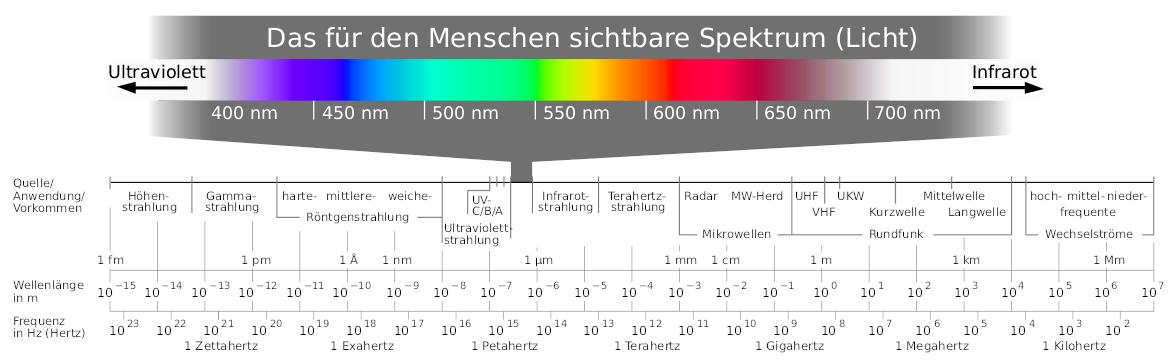
\includegraphics[width=1.0\linewidth]{figures/elektro_spektrum.png}
	\caption{Elektromagnetisches Spektrum}
\end{figure}
\begin{itemize}
	\item \textbf{2.4 GHz} (1-10dm) UHF: Ultra High Frequency
	\item \textbf{5 GHz} (1-10cm) SHF: Super High Frequency
\end{itemize}
Für das 5G Netz wurden neue Frequenzbereiche festgelegt und versteigert.
\begin{itemize}
	\item Mobilfunk: 600 MHz bis 6 GHz
	\item WLAN: 24 GHz bis 40 GHz
\end{itemize}

\subsection*{Komponenten im WLAN}
\begin{itemize}
	\item Endgeräte: mit Netzwerkkarten und Antennen
	\item Wireless Router: Multifunktionsgeräte mit eingebautem Switch, Router, Modem Access Point,...
	\item Access Points: Schnittstelle zwischen dem drahtlosen Netz und dem verkabelten Netz. Man unterscheidet zwischen Autonomen-Access-Points (schwer erweiterbar) und Controller-Based-Access-Points.
\end{itemize}

\subsection*{Wifi Frame}
\begin{tabular}{|l|l|l|}
	\hline
	Frame Control & Metainformationen z.B. Protokoll, Art des Frames,... & 2 Bytes \\
	\hline
	Duration & Übertragungsdauer, aufgrund unterschiedlicher Framelänge & 2 Bytes \\
	\hline
	Address 1 & Empfänger MAC-Adresse & 6 Bytes \\
	\hline
	Address 2 & Sender MAC-Adresse & 6 Bytes \\
	\hline
	Address 3 & MAC BSSID (WLAN Segment) & 6 Bytes \\
	\hline
	Sequence Control & Hängt vom AP ab &  \\
	\hline
	Address 4 & MAC-Adresse vom Access Point & 6 Bytes \\
	\hline
	Frame Body: & Header der restlichen Layer und Daten & \\
	\hline
	FC& Fehlerüberprüfung mit CRC & 4 Bytes \\
	\hline
\end{tabular}

\subsection*{Operations-Modi}
\begin{itemize}
	\item Ad Hoc: Peer-to-Peer Netzwerk ohne Router
	\item Infrastruktur: Dahinter ein verkabeltes Netz
	\item Tethering: Hotspot zur Weiterleitung zwischen zwei Netzen 
\end{itemize}

\subsection*{Kollisionen (CSMA/CA)}
Wireless Netzwerke nutzten eine Half Duplex Medium zum Senden. Man kann zeitgleich senden und empfangen. Zusätzlich ist es ein Shared Medium, das heißt viele Teilnehmer sind mit dem gleichem Medium verbunden. Somit kann es zu Kollisionen kommen (CSMA - Carrier Sense Multiple Access). Wifi löst das Problem mit Collision Avoidance (CA), es versucht also Kollisionen zu vermeiden. Falls gerade keiner sendet wird um Zeit beim Access Point angefragt. Dann erhält man einen Zeitslot indem man seine Daten senden und empfangen kann.

\subsection*{Verbinden mit einem Accesspoint}
\begin{itemize}
	\item AP finden (aktiv, passiv)
	\item Authentifizieren: SSID, Passwort, Network Mode (a, b, g,...), Security (WPA, WPA2,...), Channel
	\item Verbindung herstellen
\end{itemize}

\subsection*{Channels}
Die Frequenzen werden in kleinere Bereiche aufgesplittet. Gleiche Channels können sich gegenseitig stören. Überlappende Access Points sollten verschiedene Channels nutzen.
\begin{itemize}
	\item 2.4 GHz: Europa 13 Channels (1, 6 \& 11 nicht überlappend)
	\item 5 GHz: 24 Channels (alle ohne Überlappung)
\end{itemize}

\subsection*{WLAN-Angriffe}
\begin{itemize}
	\item Datendiebstahl: Shared medium $\rightarrow$ Verschlüsselung
	\item DoS: falsch konfiguriert, Störsender,...
	\item Rogue Access Point: zusätzlichen falschen AP ins Netz eingefügt
	\item Evil Twin: einen AP einfügen, der gleich aussieht aber in ein anderes Netz führt
\end{itemize}

\subsection*{Sicherheit und Verschlüsselung}
\begin{itemize}
	\item SSID Beacon verbergen (passic)
	\item MAC-Adressen filtern (L2 Security)
	\item Authentifizierung
	\begin{itemize}
		\item \textbf{Open:} ohne Password (nicht empfohlen)
		\item \textbf{Shared Key:} WEP, WPA (TKIP+AES), WPA2, WPA3
	\end{itemize}
\end{itemize}

Bei WPA2 unterscheidet zwei Varianten zum Authentifizieren:
\begin{itemize}
	\item \textbf{Personal:} ein Passwort für alles (PSK, Pre Shared Key), eher im privaten Bereich
	\item \textbf{Enterprise:} Anmeldung mit Username und Passwort, man meldet sich bei einem Server (z.B. RADIUS), eher im Firmenbereich
\end{itemize}

\subsection*{WPA2-Personal Handshake: Pre-Shared-Key (4-Way)}
Zum Austausch der Schlüssel zwischen dem Access Point und dem Client findet ein 4-Way-Handshake statt. Dabei werden die benötigten Schlüssel generiert. Zum Generieren der Schlüssel muss das Passwort nie übertragen werden, deshalb nennt man die Variante auch PSK (Pre-Shared-Key). Der Schlüssel wurde also davor schon ausgemacht.

\begin{figure}[H]
	\centering
	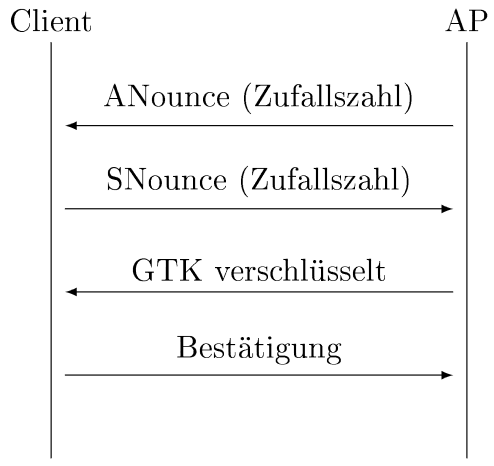
\includegraphics[width=0.8\linewidth]{figures/wpa2_personal_handshake.png}
	\caption{WPA2 Personal Handshake}
\end{figure}
\textbf{PTK (Pairwise Transient Key):} für Unicasts, jeder hat seinen eigenen Schlüssel mit dem AP \\
\textbf{PTK = PRF(Pwd+ANounce+SNounce+APMAC+ClientMAC)} \\
\textbf{PRF (Pseudo Random Function):} ist eine Pseudo-Zufallsfunktion die dann den Schlüssel erzeugt und den Geräten bekannt ist. \\
\textbf{GTK (Group Temporal Key):} für Broadcast und Multicasts im Netz, für alle Teilnehmer gleich.

Das Passwort wird nie über das Medium ausgetauscht, deshalb nennt man das Verfahren Pre Shared Key. Die Nachricht wird nach Layer 2 verschlüsselt. Dieser kann nicht verschlüsselt werden, da der Access Point die Frames identifizieren muss. Danach im verkabelten Netz, wie sonst auch immer, wird wieder nach Layer 4 verschlüsselt (z.B. mit TLS).
	\chapter{Network Security}
Netzwerkangriffe können auf unterschiedliche Arten, unterschiedlichen Ebenen und verschiedene Protokolle stattfinden. Deshalb muss bei einem Security-Konzept möglichst alles berücksichtigt werden.
\begin{table}[H]
	\begin{tabular}{|l|l|l|}
		\hline
		\multicolumn{1}{|c|}{\textbf{Angriffe}} & \multicolumn{1}{c|}{\textbf{OSI-Modell}} & \multicolumn{1}{c|}{\textbf{Abwehr}} \\ \hline
		\begin{tabular}[c]{@{}l@{}}Social Engineering\\ Passwörter\\ Pretexting\end{tabular} & L8-Mensch & \begin{tabular}[c]{@{}l@{}}Schulungen\\ Vernünftig und vorsichtiges \\ handeln\end{tabular} \\ \hline
		\begin{tabular}[c]{@{}l@{}}SQL-Injection\\ Wurm, Virus, Trojaner\\ Ransomware, Spyware\\ Protokolle (HTTP, FTP, \\ Telnet, DHCP, DNS,...)\end{tabular} & \begin{tabular}[c]{@{}l@{}}L7-Application\\ L6-Presentation\\ L5-Session\end{tabular} & \begin{tabular}[c]{@{}l@{}}Firewall, IPS, IDS, ESA, WSA\\ Eingabeüberorpfung\\ gute Software \& Protokolle\\ End-Point-Detection\\ Anti-Virus, Updates\end{tabular} \\ \hline
		\begin{tabular}[c]{@{}l@{}}DDOS\\ $\rightarrow$ TCP (SYN-Flood,\\ $\rightarrow$ UDP\end{tabular} & L4-Transport & \begin{tabular}[c]{@{}l@{}}IPS, IDS\\ Firewall, ACL\end{tabular} \\ \hline
		\begin{tabular}[c]{@{}l@{}}Routing, DDoS\\ MITM, IP-Spoofing\\ Protokolle (ICMP,\end{tabular} & L3-Network & \begin{tabular}[c]{@{}l@{}}Firewall, ACL, IPS, IDS\\ sichere Protokolle (IPsec)\end{tabular} \\ \hline
		\begin{tabular}[c]{@{}l@{}}MITM: ARP-Spoofing, MAC-Spoofing\\ DDOS: MAC-Flooding\\ Protokolle (STP, CDP)\end{tabular} & L2-Data Link & \begin{tabular}[c]{@{}l@{}}MAC-Filter, AAA\\ sichere Protokolle\\ Verschlüsselung\end{tabular} \\ \hline
		\begin{tabular}[c]{@{}l@{}}DoS (Störsender, Zerstörung \\ der Infrastruktur)\\ Physischer Zugang\\ MITM, Hardware\end{tabular} & L1-Physical & \begin{tabular}[c]{@{}l@{}}Zutrittskontrolle\\ Backups\end{tabular} \\ \hline
	\end{tabular}
\end{table}
Dem Angreifer reicht eventuell ein einziger Angriffspunkt im Netz. Meist sind die User (Personen) das größte Problem. $\rightarrow$ ''Der Angreifer muss nur einmal gewinnen''

\textbf{Sicherheitsrichtlinien} \\
\begin{tabular}{ | p{\dimexpr 0.5\linewidth-2\tabcolsep} | p{\dimexpr 0.5\linewidth-2\tabcolsep} |} \hline
	\textbf{User} & \textbf{Unternehmen} \\ \hline
	$\bullet$ Passwörter (Mindestlänge, eins pro Account, keine persönlichen Daten) & $\bullet$ Passwortrichtlinien, User Verwaltung, Recht vergeben \\
	$\rightarrow$ Passwortmanager, 2FA & $\bullet$ Firmengeräte, spezielle Rechte, wie beim User \\
	$\bullet$ Datenverwaltung (Wann?, Wo?, Welche?, Wann?,...) & $\bullet$ DMZ, VPN, Firewall, IPS, IDS, WSA, ESA \\
	$\bullet$ Firewall & $\bullet$ Zugangskontrollen \\
	$\bullet$ Updates (OS, Software) & $\bullet$ Schulung der Mitarbeiter \\
	$\bullet$ Antivirus/Antispysoftware & $\bullet$ Backups \\
	$\bullet$ Vernünftig handeln & $\bullet$ Pen-Testing \\
	 & $\bullet$ Risikoanalyse $\rightarrow$ Schwachstellen kennen \\
	 & $\bullet$ Verhaltensanalyse \\
	 & $\bullet$ Datatransfer sichtbar machen \\
	\hline
\end{tabular} 

\section{Firewall}
Mit einer Firewall kann der eingehende/ausgehende Datenverkehr kontrolliert, protokolliert und gefiltert werden (sperren, freigeben).

\textbf{Unterscheidung nach Position}
\begin{itemize}
	\item \textbf{Personal Firewall} (am eigenen Gerät) z.B. Windows Defender, UFW,...
	\item \textbf{External Firewall} (zwischen lokalen \& globalen Netz) z.B. ASA, Fortinet, Barracuda, PFSense,...
\end{itemize}

\textbf{Unterscheidung nach Funktion}
\begin{itemize}
	\item (L4) \textbf{Paketfilter:} IP-Adressen, Ports z.B. ACL
	\item (L4) \textbf{Stateful Inspection:} Untersucht die ganze Sitzung (mehrere Aufrufe zu z.B. gleiche IPs)
	\item (L7) \textbf{Application Firewall:} Proxy Server
	\item (Daten) \textbf{Deep Paket Inspection Firewall}
\end{itemize}

Eine falsch konfigurierte Firewall bietet keinen Schutz. Eine Firewall muss ständig gewartet und aktualisiert werden.

\section{IDS \& IPS}
\begin{figure}[H]
	\centering
	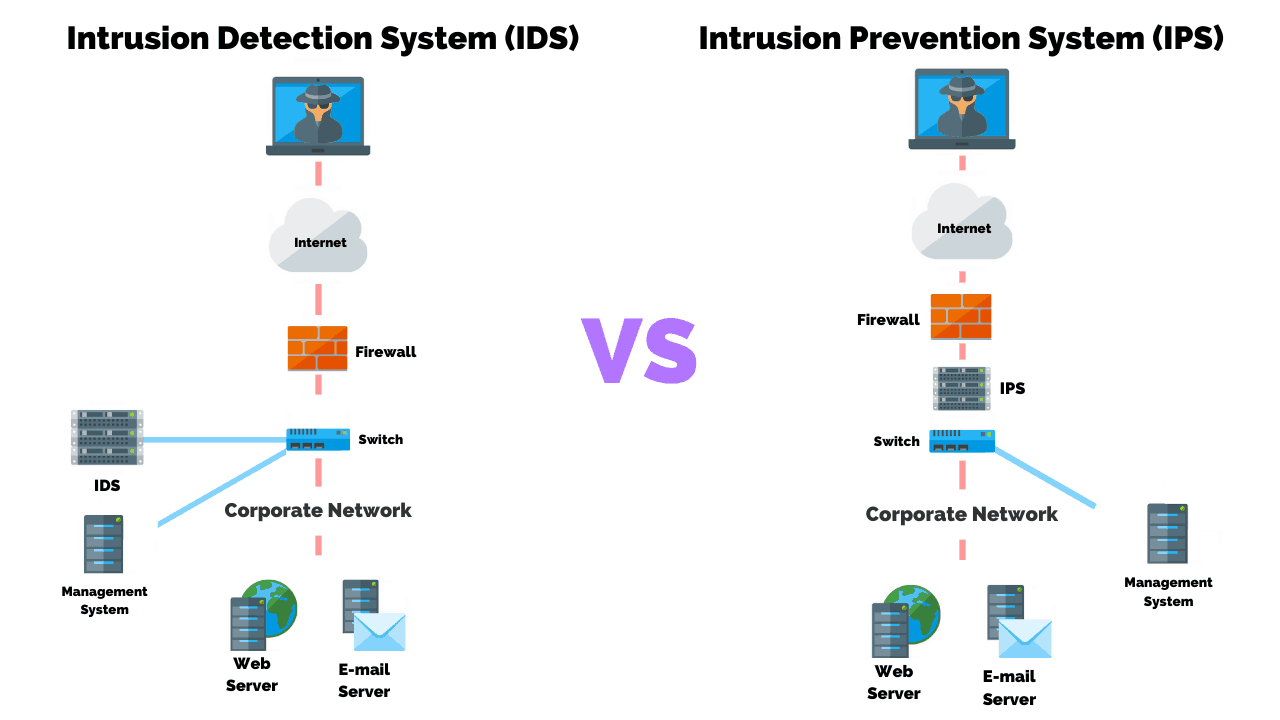
\includegraphics[width=0.8\linewidth]{figures/ids_ips.png}
	\caption{IPS \& IDS}
\end{figure}

\begin{tabular}{ | p{\dimexpr 0.5\linewidth-2\tabcolsep} | p{\dimexpr 0.5\linewidth-2\tabcolsep} |} \hline
	\textbf{IDS (Intrusion Detection System)} & \textbf{IPS (Intrusion Prevention System)} \\ \hline
	Wird nur parallel informiert & Alles muss über IPS \\
	+ schneller (da es parallel ist) & - langsamer (da seriell) \\
	- nur Warnungen & + sicherer \\
	\hline
\end{tabular} 

\section{Honeypot}
\begin{figure}[H]
	\centering
	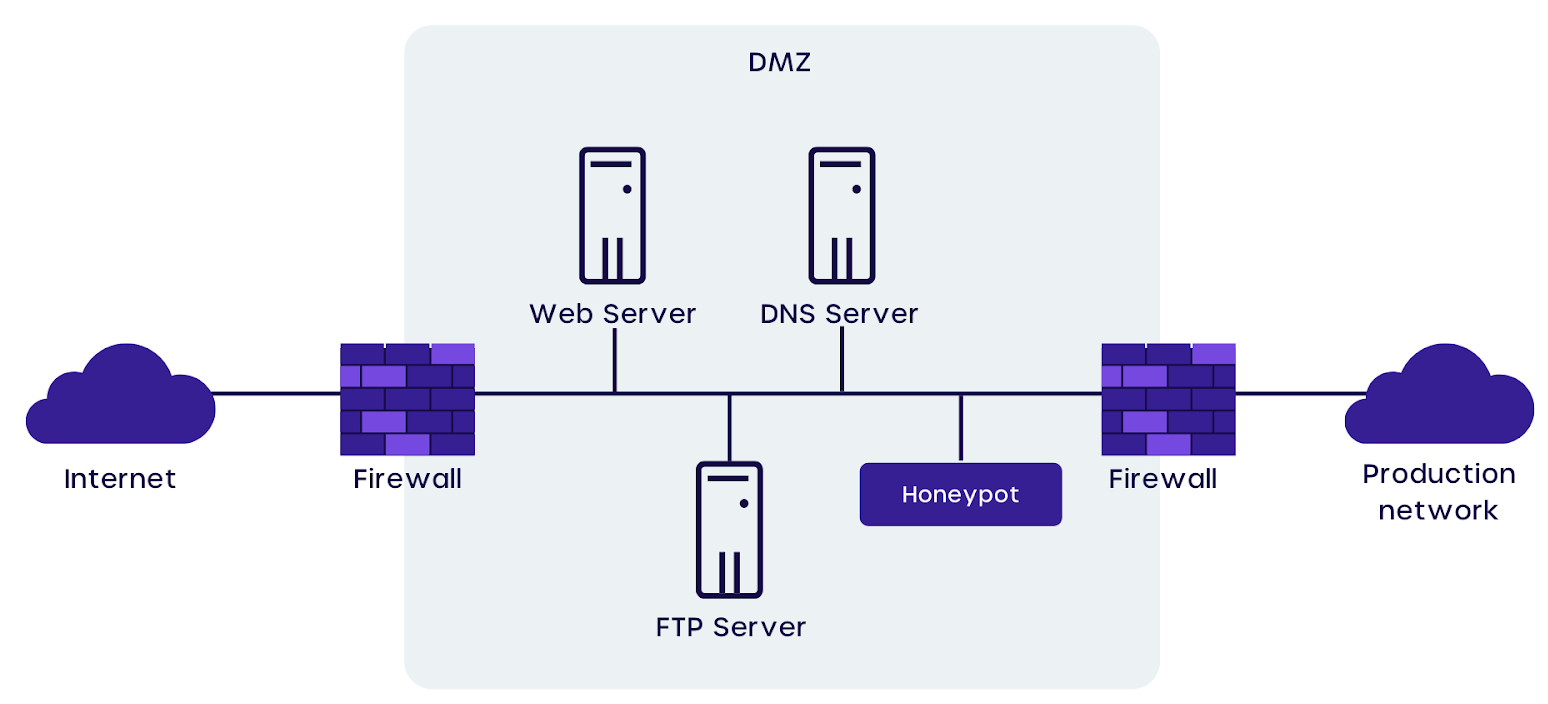
\includegraphics[width=0.8\linewidth]{figures/honeypot.png}
	\caption{Honeypot}
\end{figure}
Bei einem Honeyport werden bewusst veraltete Software \& Hardware für Angreifer als Köder aufgestellt. 

\section{VPN} 
Erstellt eine verschlüsselte Verbindung zu einem entfernten VPN-Server.

\begin{figure}[H]
	\centering
	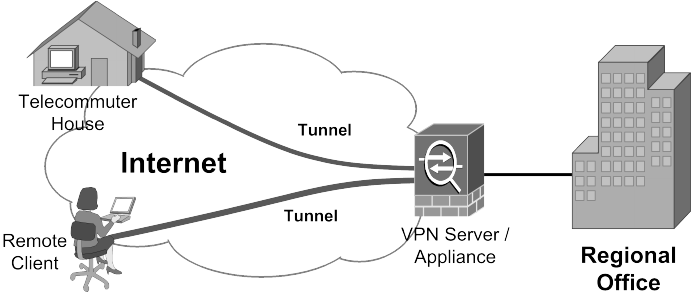
\includegraphics[width=0.8\linewidth]{figures/vpn.png}
	\caption{VPN}
\end{figure}

Arten von VPN:
\begin{itemize}
	\item Ende-zu-Ende VPN
	\item Ende-zu-Netz VPN
	\item Netz-zu-Netz VPN
\end{itemize}

\section{ESA (Email Security Appliance) \& WSA (Web Security Appliance)}
Funktioniert wie ein Proxy-Server.
\begin{figure}[H]
	\centering
	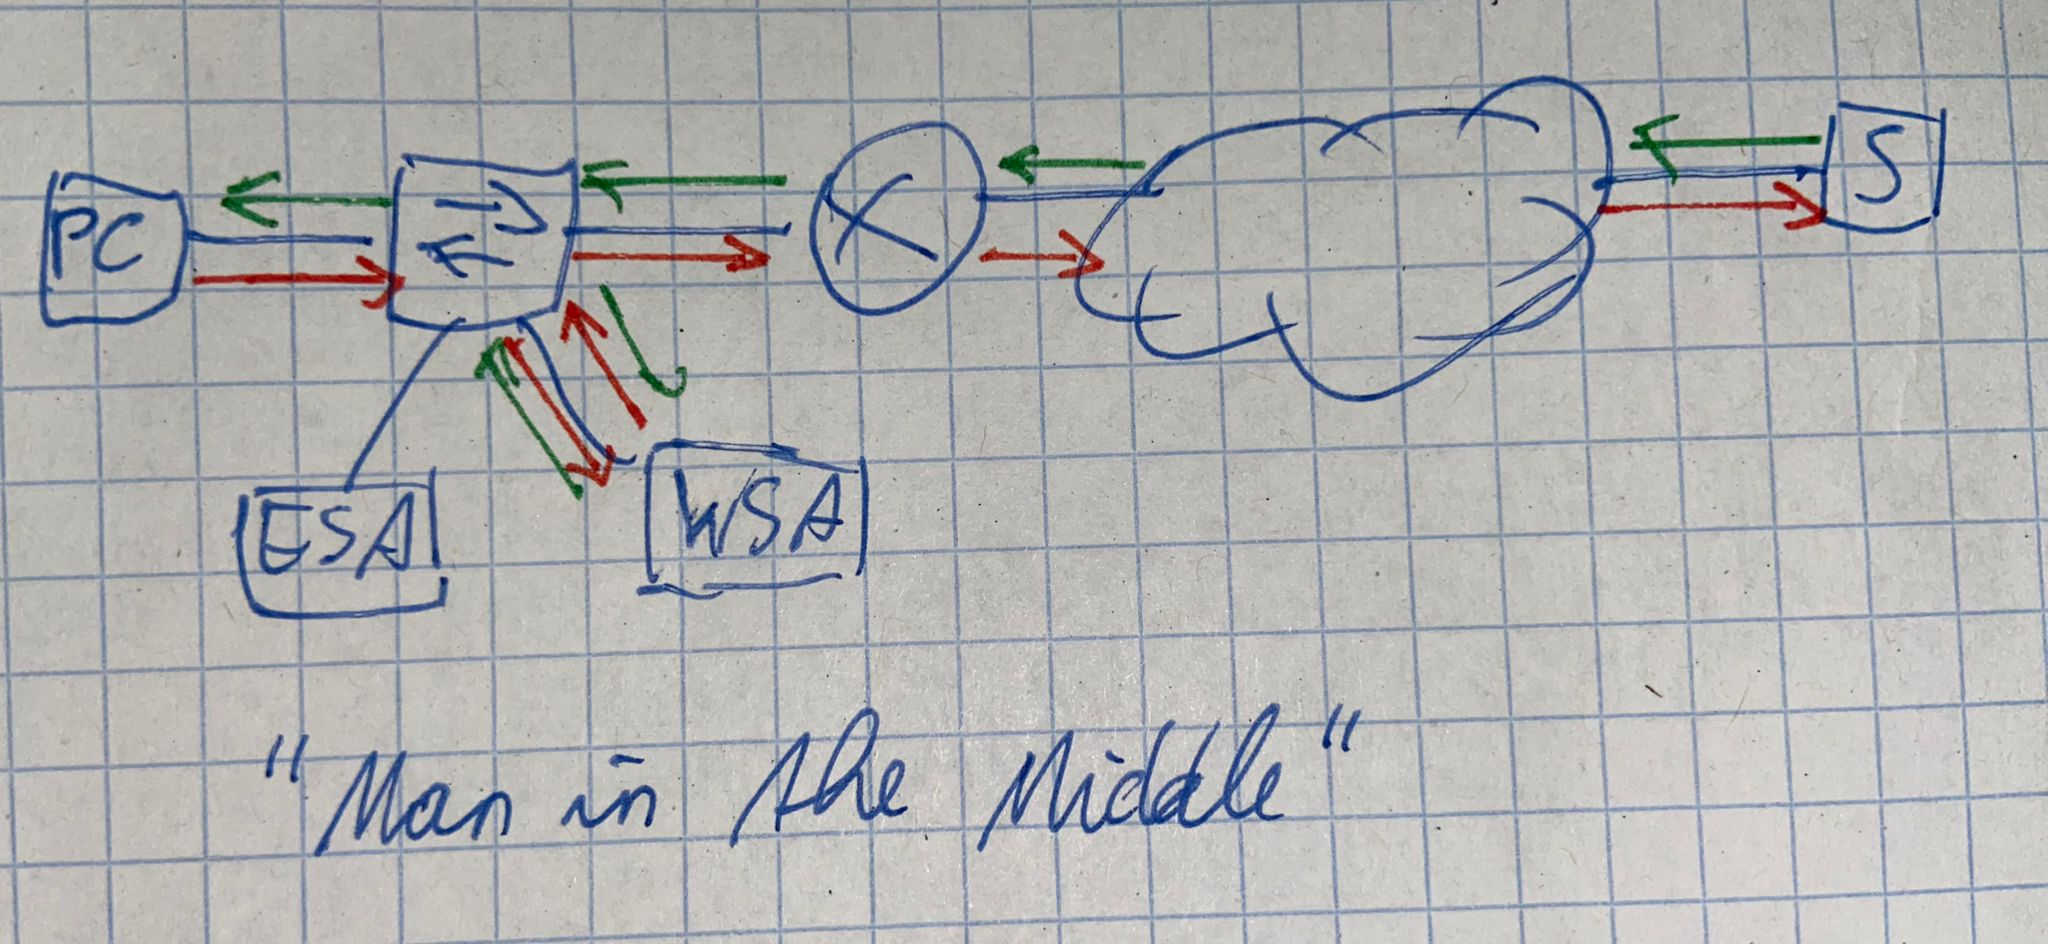
\includegraphics[width=0.8\linewidth]{figures/esawsa.jpeg}
	\caption{ESA \& WSA}
\end{figure}

\section{IPsec}
Ziel: Sicheres Protokoll zur Datenübertragung
\begin{itemize}
	\item \textbf{Transport-Modus:} Verschlüsselung ab L4 und fügt eine Authentifizierung in den Header ein.
	\item \textbf{Tunnel-Modus:} Alles wird verschlüsselt und es wird ein neuer verschlüsselter Header angehängt. Darin stehen die wichtigsten Felder (MAC, IP,...) + Authentifizierung
\end{itemize}
	\chapter{Hashfunktionen}
Bei einer Hashfunktion ist die Wertemenge meist wesentlich kleiner als die Lösungsmenge. \\
Die Elemente der Wertmenge können normalerweise eine beliebige Länge haben. \\
Die Elemente der Lösungsmenge haben meist eine fixe Länge.

\begin{tabbing}
	$\bullet$ Anfangsbuchstabe: ~~~~ \= Hallo $\rightarrow$ H \\
	~~~~~~~~~~~~~~~~~~~~~~~~~~~~~~~~ \= Tim $\rightarrow$ T \\
	$\bullet$ Postleitzahl: ~~~~~ \= Grins $\rightarrow$ 6591 \\
	~~~~~~~~~~~~~~~~~~~~ \= Neustift $\rightarrow$ 6167 \\
	$\bullet$ CRC ...
\end{tabbing}

\section{Kryptographische Hashfunktionen}
Kryptographische Hashfunktionen müssen spezielle Eigenschaften erfüllen. Die wichtigste Eigenschaft ist, dass es sich um eine Einwegfunktion handelt.
\begin{figure}[H]
	\centering
	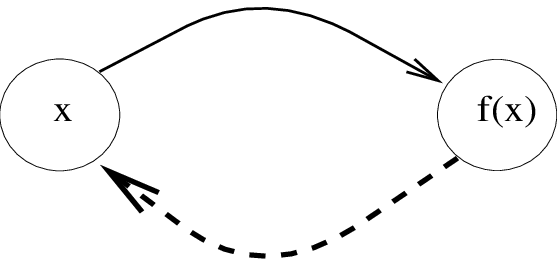
\includegraphics[width=0.6\linewidth]{figures/oneway.png}
	\caption{Einwegfunktion}
\end{figure}

\subsection*{Eigenschaften}
\begin{itemize}
	\item \textbf{Einwegfunktion:} Unumkehrbarkeit muss so gut wie möglich gegeben sein
	\item Diffusion ('Lawineneffekt'): kleine Änderung in der Eingabe bewirkt die ganze Ausgaben.
	\item Konfusion: Von Hashwert kann man keine Rückschlüsse auf den Eingabewert machen
	\item Eindeutigkeit
	\item Kollisionsresistenz: Die Wahrscheinlichkeit, dass Kollisionen vorkommen soll so klein wie möglich sein (im besten Fall gleich Null sein)
\end{itemize}

\subsection*{Hash-Algorithmen}
\begin{itemize}
	\item MD5: 128 Bit Hashwert, unsicher!
	\item SHA (secure hash algorithm)
	\begin{itemize}
		\item SHA1: 160 Bit Hashwerte unsicher!
		\item SHA2 \\
		$\rightarrow$ SHA224, SHA256, SHA 384, SHA512
		\item SHA3: grundlegend anders, 224, 256, 384 Bitwerte $\rightarrow$ auch frei wählbar
	\end{itemize}
	\item GOST, Whirlpool
\end{itemize}

\subsection*{Ablauf SHA-256} 
\begin{itemize}
	\item Block erstellen (Auffüllen, Startblock erstellen, Wurzel von Primzahlen)
	\item Bitrotation, Zeilen integrieren (Diffusion)
	\item XOR, Bitshift (viele Runden)
	\item Auswahlfunktion, Mehrheitsfunktion (Einwegfunktion)
\end{itemize}

\textbf{Zusatz:} Message Authentication Code z.B. HMAC: Schlüssel-Hash-Nachtrichtauthentifizierung, Pre-Shared-Key

\subsection*{Angriffe}
\begin{itemize}
	\item Brute-Force
	\item Phising
	\item Wörterbuchangriff
	\item Algorithmus mutzen
	\item Rainbow-Table (viel Speicher) \\
	$\rightarrow$ viele Hashwerte als Kette gespeichert
\end{itemize}

\section{Passwörter}
\begin{enumerate}
	\item \textbf{lokale Speicherung}
	\begin{itemize}
		\item Länge des Passworters (mind 12 Zeichen)
		\item keine Wörter, persönliche Informationen
		\item Buchstaben/Zahlen/Symbole
		\item Jedes Passwort nur einmal verwenden
		\item Passwortmanager verwenden oder MFA als Alternative
	\end{itemize}
	\item \textbf{Speicherung am Server}
	\begin{itemize}
		\item \textbf{Klartext} \Lightning: Zugriff auf Datenbank, Admin, MITM
		\item \textbf{Gehashed} \Lightning: MITM, gleiche Passwörter erkennbar
		\item \textbf{Gehashed + Salt:} Mitm, Brute-Force
		\item \textbf{Gehashed + Salt + Pepper} \\
		\textbf{Salt:} Zufällige Zeichenkette die im Klartext in der Datenbank gespeichert wird $\rightarrow$ Jeder bekommt eigenen Hashwert \\
		\textbf{Pepper:} Zufällige Zeichenkette die NICHT in der Datenbank steht
	\end{itemize}
	\item \textbf{Austausch Client-Server}
	\begin{itemize}
		\item PAP unsicher! 
		\begin{figure}[H]
			\centering
			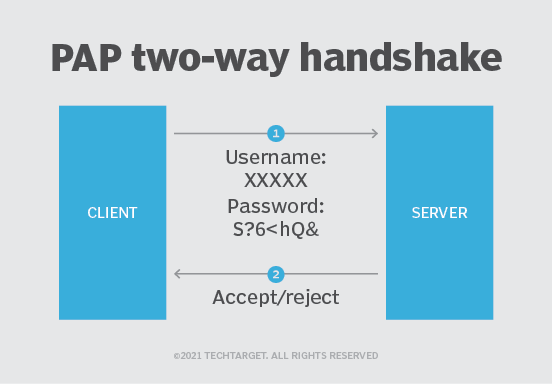
\includegraphics[width=0.6\linewidth]{figures/pap.png}
			\caption{PAP}
		\end{figure}
		\item CHAP: Bei CHAP wird bei jedem Anmeldeversuch eine Challenge (Zufallszahl) gesendet. Der Client hashed sein Passwort mit der Zufallszahl und sendet es dem Server. Der Server kann dann das Passwort in der Datenbank mit der gesendeten Zufallszahl hashen und es mit dem Client-Hash vergleichen. Somit wird zum einem, das Passwort nie im Klartext gesendet und zum anderen kann der gesendete Hash nicht nocheinmal gesendet werden, da die Zufallszahl 'einzigartig' ist und bei jedem Anmeldeversuch anders ist. \\
		$\rightarrow$ MITM Anmeldung mit dem Hashwert ist durch die Challenge nicht mehr möglich
		\begin{figure}[H]
			\centering
			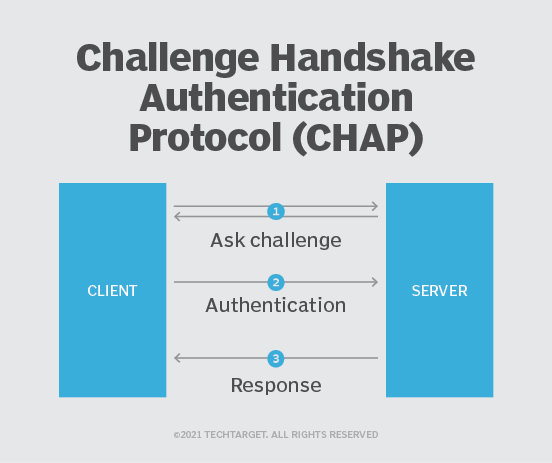
\includegraphics[width=0.6\linewidth]{figures/chap.png}
			\caption{PAP}
		\end{figure}
		\textbf{Alternativen:} MS-CHAPv1, MSCHAPv2, EAP, PEAP,...
	\end{itemize}
\end{enumerate}

\section{AAA}
Autorisierung (Was?), Authentifizierung (Wer?) \& Accounting (Wann?) \\
Protokolle: RADIUS, TACACS+

\section{PKI (Public Key Infrastruktur)}
Digitale Zertifikate sind für die Authentifizierung eines öffentlichen Schlüssels und seiner zulässigen Anwendung bzw. Geltungsbereich 

\begin{tabbing}
	Vergleich: ~~~~~~~~ \= Zertifikat $\rightarrow$ Pass \\
	~~~~~~~~~~~~ \= digitale Signatur $\rightarrow$ Foto
\end{tabbing}

\begin{figure}[H]
	\centering
	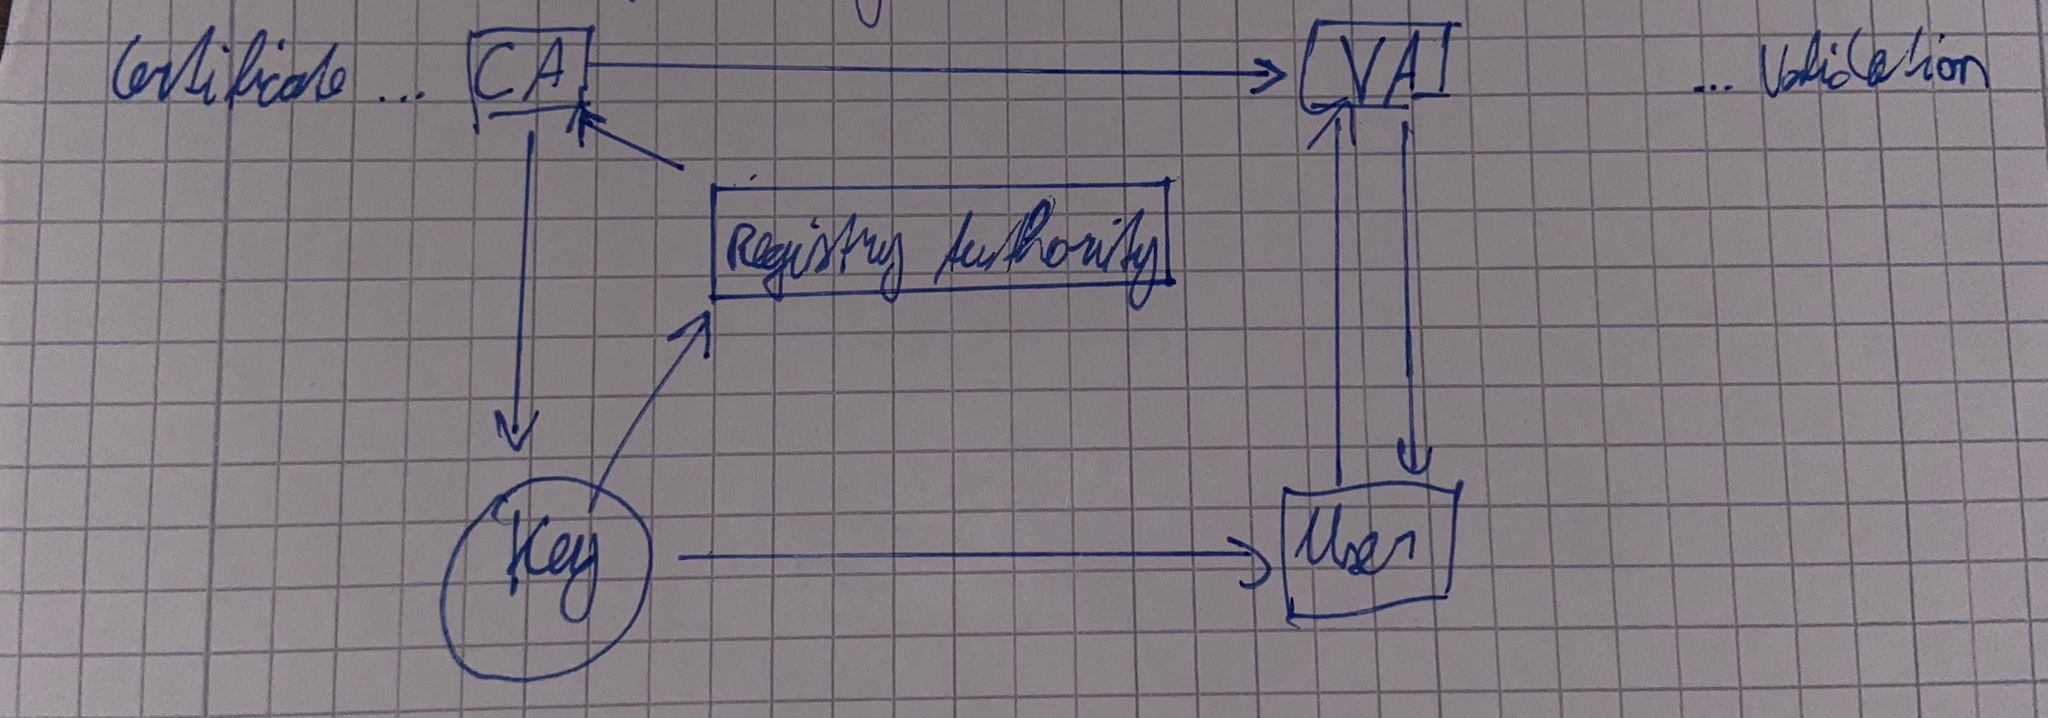
\includegraphics[width=0.7\linewidth]{figures/cert.jpeg}
	\caption{Public Key Infrastruktur}
\end{figure}

\textbf{Alternative:} Web of Trust \\

\section{Zusammenfassung}
\begin{tabular}{ | p{\dimexpr 0.5\linewidth-2\tabcolsep} | p{\dimexpr 0.5\linewidth-2\tabcolsep} |} \hline
	\textbf{verwendete Algorithmen} & \textbf{typische Protokolle} \\ \hline
	AES/DES & HTTPS \\
	RSA & IPsec \\
	Diffie-Hellman & VPN \\
	Hashfunktionen (SHA256,...) & SSH \\
	MAC (bzw. HMAC) & PSK (WLAN) \\
	Authentifizierung (AAA, CHAP) & RADIUS \\
	PKI & ... \\
	\hline
\end{tabular} 

\section{HTTPS:} HTTP + TLS (SSL)
TLS ... transport layer security, Verschlüsselung nach Layer 4
\begin{itemize}
	\item Symmetrische Verschlüsselung
	\item Asymmetrischer Schlüsselaustausch (ab TLS 1.3 Diffie-Hellman)
	\item Authentifizierung (Server), PKI, RSA
	\item Hashfunktionen (SHA256,...)
	\item Sicherung der Nachrichtenintegrität (HMAC)
\end{itemize}

\begin{figure}[H]
	\centering
	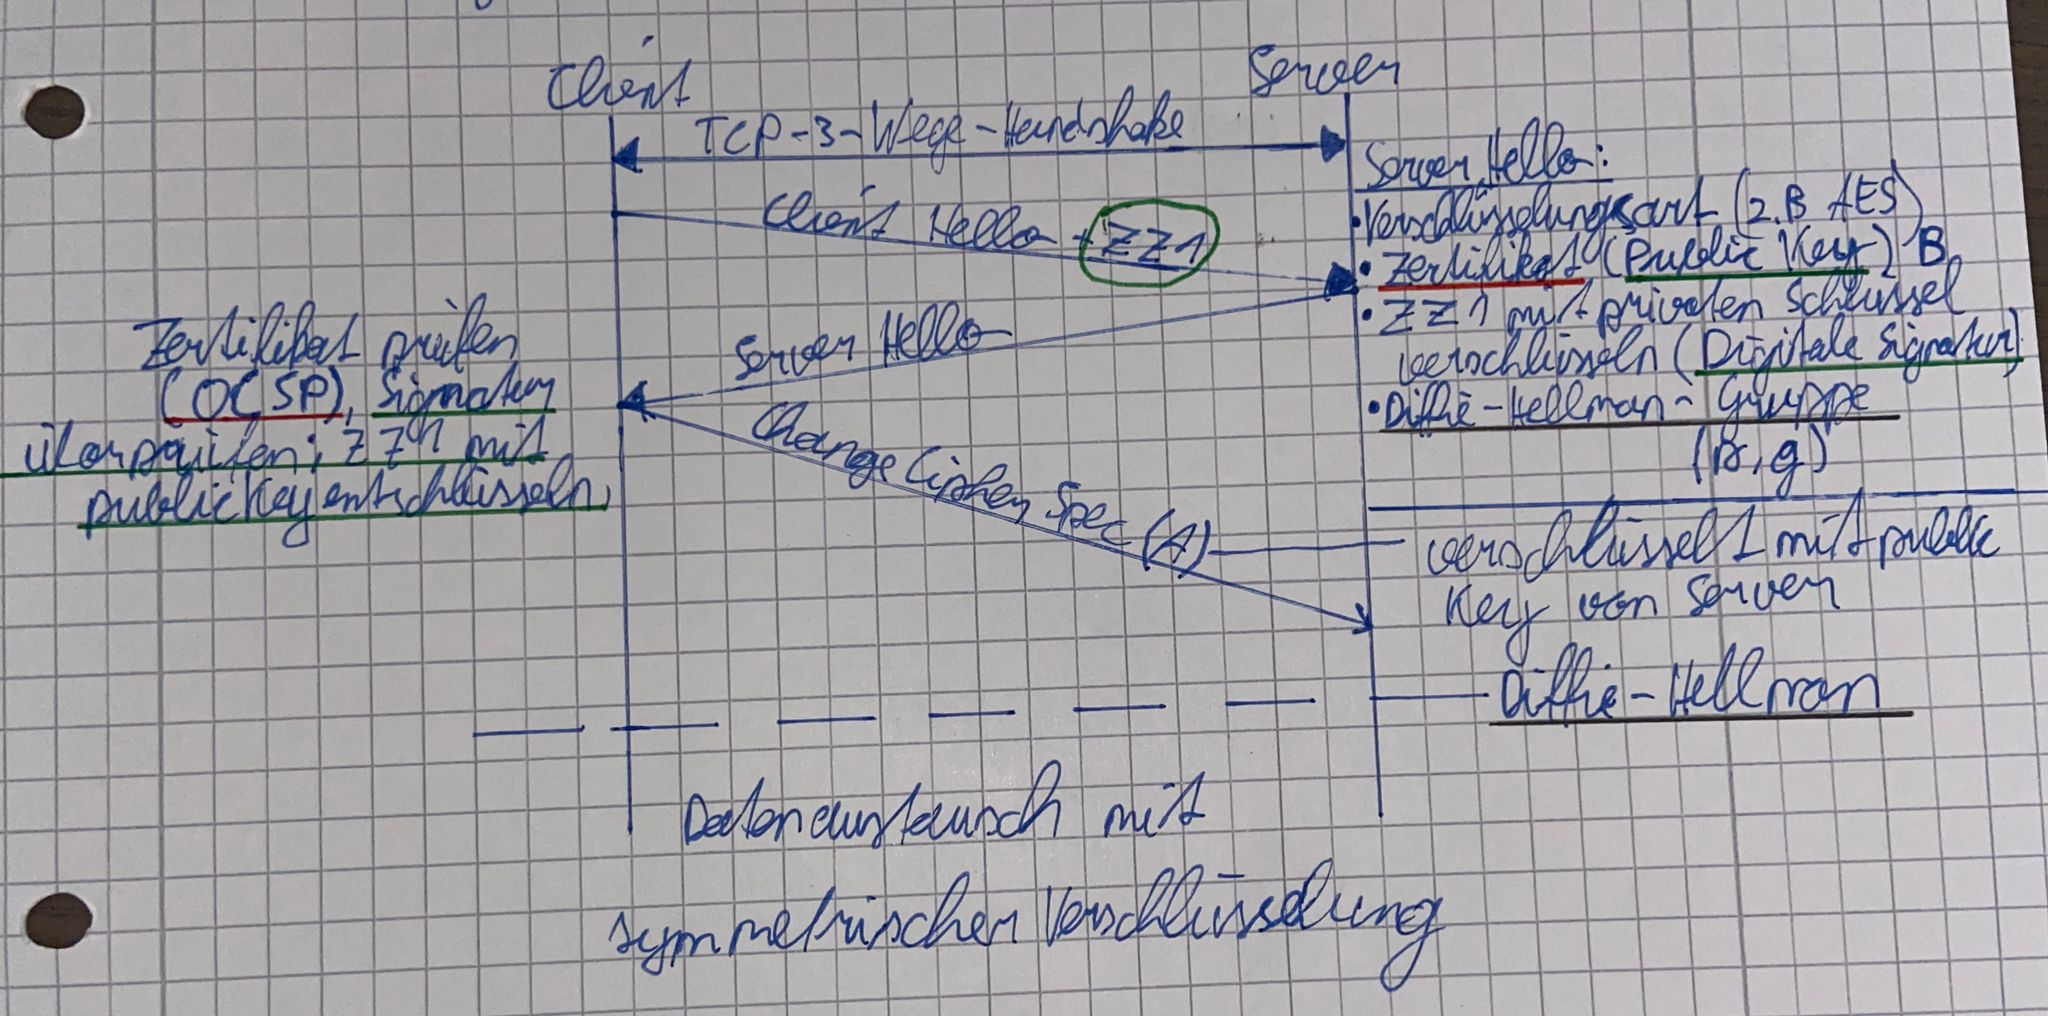
\includegraphics[width=1.0\linewidth]{figures/https.jpeg}
	\caption{HTTPS Verbindungsaufbau}
\end{figure}










	
	%\chapter{template}
\section{image}

\begin{figure}[H]
	\centering
	
\includegraphics[width=0.8\linewidth]{figures/test.jpg}
	\caption{image example}
\end{figure}

\section{code}
Quellcode \ref{code:code_ex} 

\lstinputlisting[style=Java, label={code:code_ex}, caption={code include example}, captionpos=b]{code/code.java}
	
	
%-------------------------------------------------------------------------------------------%
% VERZEICHNISSE
	\pagenumbering{Roman}
	\setcounter{chapter}{0}
	\renewcommand{\thechapter}{\Roman{chapter}} 

	\listoffigures

	%\listoftables	
	
	\lstlistoflistings
	
	%\printbibliography

\end{document}